\KOMAoption{paper}{a4, portrait}
\areaset{267mm}{180mm}
\fancyheadoffset{0pt} % обновляем хедер и футер

\newgeometry{
  top=14mm,
  bottom=11mm,
  right=10mm,
  left=22mm,
}

\begin{landscape}

%\setlength{\headsep}{5.6mm} 
%\setlength{\topmargin}{-27mm}
\setlength{\footskip}{15.5pt}
%\setlength{\textwidth}{305mm}

\color{unimain}{\section[(справочное) Перечень сигналов ФСУ, предназначенных \newline для конфигурирования устройства <<ЮНИТ-М300-ОЛ>>]{(справочное)\\Перечень сигналов ФСУ, предназначенных для конфигурирования устройства <<ЮНИТ-М300-ОЛ>>}\label{app:signals}}
\color{black}

\begin{enumerate}[label=\ref{app:signals}.\arabic*] % Без глобального влияния
  \item Перечень сигналов самодиагностики, доступных для конфигурирования, приведен в документации ЮТКБ.656122.609 РЭ <<Устройство защиты и автоматики серии <<ЮНИТ-М300>>. Руководство по эксплуатации общее>>.
  \item Условные обозначения, применяемые в таблице перечня сигналов:
  \begin{itemize}
    \item[$\text{(--)}$] { - сигнал не имеет возможности конфигурации на данный параметр;}
    \item[$\text{(+)}$] { - сигнал имеет возможность конфигурации на данный параметр.}
  \end{itemize}
\end{enumerate}

\small % сделаем шрифт в таблице поменьше
% В таблице ниже убрал правую и левую горизонтальные линии чтобы не сливались и жирно видно - также в настройках geometry прищлось поле right =8mm а не 5 mm 
% так как строки ниже колонтитулов спускались
\begin{longtable}{
>{\centering\arraybackslash}m{6.0cm}
|>{\centering\arraybackslash}m{3.45cm}
|>{\centering\arraybackslash}m{2cm}
|>{\centering\arraybackslash}m{2cm}
|>{\centering\arraybackslash}m{2cm}
|>{\centering\arraybackslash}m{2cm}
|>{\centering\arraybackslash}m{2cm}
|>{\centering\arraybackslash}m{2cm}
|>{\centering\arraybackslash}m{2.107cm}
}

%\caption{Перечень сигналов ФСУ, предназначенных для конфигурирования устройств ЮНИТ-М300\vspace{-0.5\baselineskip}}\label{appA:tbl1}\\ % выравнивает надпись посередине таблицы
\caption{Перечень сигналов ФСУ, предназначенных для конфигурирования устройства\hfill\vspace{-0.5\baselineskip}}\label{appA:tbl1}\\ 

\hline
\rowcolor{unimain!40}
Полное наименование сигнала & Наименование сигнала на ФСУ & Дискретные входы & Выходные реле & Светодиоды & Функционал. клавиши & Регистратор событий & Аварийный осциллограф & Пуск авар. осциллографа \\ 
\hline
\endfirsthead
%\caption{\emph{Продолжение\vspace{-0.5\baselineskip}}} \\ % Отступ обозначения таблицы от таблицы и выравнивание надписи слева
\caption*{\hspace{3pt}\emph{Продолжение таблицы \ref{appA:tbl1}\hfill\vspace{-0.5\baselineskip}}} \\ % сделано по ГОСТ 2.105 п.6.8.7
\hline
\rowcolor{unimain!40}
Полное наименование сигнала & Наименование сигнала на ФСУ & Дискретные входы & Выходные реле & Светодиоды & Функционал. клавиши & Регистратор событий & Аварийный осциллограф & Пуск авар. осциллографа \\ 
%\hline
\endhead

%\hline
\endfoot

%\hline
\endlastfoot

%===t2
\rowcolor{gray!10}
\multicolumn{9}{c}{Общие сигналы ФС} \\
\hline
\raggedright Разрешить включение выкатного элемента & \centering ВЭ. Разрешить вкл & \centering -- & \centering -- & \centering -- & \centering -- & \centering + & \centering + & \centering \arraybackslash + \\ \hline
\raggedright Разрешить отключение выкатного элемента & \centering ВЭ. Разрешить откл & \centering -- & \centering -- & \centering -- & \centering -- & \centering + & \centering + & \centering \arraybackslash + \\ \hline
\raggedright Разрешить включение заземляющего ножа & \centering ЗН. Разрешить вкл & \centering -- & \centering -- & \centering -- & \centering -- & \centering + & \centering + & \centering \arraybackslash + \\ \hline
\raggedright Разрешить отключение заземляющего ножа & \centering ЗН. Разрешить откл & \centering -- & \centering -- & \centering -- & \centering -- & \centering + & \centering + & \centering \arraybackslash + \\ \hline
\raggedright Выключатель отключен (блок контакт) & \centering В отключен (б/к) & \centering + & \centering + & \centering + & \centering -- & \centering + & \centering + & \centering \arraybackslash + \\ \hline
\raggedright Выключатель включен (блок контакт) & \centering В включен (б/к) & \centering + & \centering + & \centering + & \centering -- & \centering + & \centering + & \centering \arraybackslash + \\ \hline
\raggedright Ключ М/Д привода В & \centering Ключ М/Д привода В & \centering + & \centering + & \centering + & \centering -- & \centering + & \centering + & \centering \arraybackslash + \\ \hline
\raggedright Низкий уровень изоляции В & \centering Низ.уров.изоляц. В & \centering + & \centering + & \centering + & \centering -- & \centering + & \centering + & \centering \arraybackslash + \\ \hline
\raggedright Аварийный уровень изоляции В & \centering Авар.уров.изоляц. В & \centering + & \centering + & \centering + & \centering -- & \centering + & \centering + & \centering \arraybackslash + \\ \hline
\raggedright Пружина не заведена & \centering Пружина не заведена & \centering + & \centering + & \centering + & \centering -- & \centering + & \centering + & \centering \arraybackslash + \\ \hline
\raggedright Контроль цепи ЭМВ & \centering Контроль цепи ЭМВ & \centering + & \centering + & \centering + & \centering -- & \centering + & \centering + & \centering \arraybackslash + \\ \hline
\raggedright Контроль цепи ЭМО1 & \centering Контроль цепи ЭМО1 & \centering + & \centering + & \centering + & \centering -- & \centering + & \centering + & \centering \arraybackslash + \\ \hline
\raggedright Контроль цепи ЭМО2 & \centering Контроль цепи ЭМО2 & \centering + & \centering + & \centering + & \centering -- & \centering + & \centering + & \centering \arraybackslash + \\ \hline
\raggedright Контроль оперативного тока ЭМО1, ЭМВ & \centering ОТ цепей ЭМО1,ЭМВ & \centering + & \centering + & \centering + & \centering -- & \centering + & \centering + & \centering \arraybackslash + \\ \hline
\raggedright Контроль оперативного тока ЭМО2 & \centering ОТ цепей ЭМО2 & \centering + & \centering + & \centering + & \centering -- & \centering + & \centering + & \centering \arraybackslash + \\ \hline
\raggedright Работа ЭМВ & \centering Работа ЭМВ & \centering + & \centering + & \centering + & \centering -- & \centering + & \centering + & \centering \arraybackslash + \\ \hline
\raggedright Работа ЭМО1 & \centering Работа ЭМО1 & \centering + & \centering + & \centering + & \centering -- & \centering + & \centering + & \centering \arraybackslash + \\ \hline
\raggedright Работа ЭМО2 & \centering Работа ЭМО2 & \centering + & \centering + & \centering + & \centering -- & \centering + & \centering + & \centering \arraybackslash + \\ \hline
\raggedright Внешняя блокировка управления В & \centering Внеш. блок. упр. В & \centering + & \centering + & \centering + & \centering -- & \centering + & \centering + & \centering \arraybackslash + \\ \hline
\raggedright Неисправность опер. тока цепей сигнализации выключателя & \centering ОТ цепей сигн. В & \centering + & \centering + & \centering + & \centering -- & \centering + & \centering + & \centering \arraybackslash + \\ \hline
\raggedright Неисправность опер. тока цепей ОБР & \centering ОТ цепей ОБР & \centering + & \centering + & \centering + & \centering -- & \centering + & \centering + & \centering \arraybackslash + \\ \hline
\raggedright Оперативно включить В & \centering Опер. включить В & \centering + & \centering + & \centering + & \centering -- & \centering + & \centering + & \centering \arraybackslash + \\ \hline
\raggedright Включить В от пульта управления & \centering Включить В от ПУ & \centering + & \centering + & \centering + & \centering -- & \centering + & \centering + & \centering \arraybackslash + \\ \hline
\raggedright Включить В от телеуправления & \centering Включить В от ТУ & \centering + & \centering + & \centering + & \centering -- & \centering + & \centering + & \centering \arraybackslash + \\ \hline
\raggedright Оперативно отключить В & \centering Опер. отключить В & \centering + & \centering + & \centering + & \centering -- & \centering + & \centering + & \centering \arraybackslash + \\ \hline
\raggedright Отключить В от пульта управления & \centering Отключить В от ПУ & \centering + & \centering + & \centering + & \centering -- & \centering + & \centering + & \centering \arraybackslash + \\ \hline
\raggedright Отключить В от телеуправления & \centering Отключить В от ТУ & \centering + & \centering + & \centering + & \centering -- & \centering + & \centering + & \centering \arraybackslash + \\ \hline
\raggedright Отключение от кнопки & \centering Откл. от кнопки & \centering + & \centering + & \centering + & \centering -- & \centering + & \centering + & \centering \arraybackslash + \\ \hline
\raggedright Заземляющий нож отключен (блок контакт) & \centering ЗН отключен (б/к) & \centering + & \centering + & \centering + & \centering -- & \centering + & \centering + & \centering \arraybackslash + \\ \hline
\raggedright Заземляющий нож включен (блок контакт) & \centering ЗН включен (б/к) & \centering + & \centering + & \centering + & \centering -- & \centering + & \centering + & \centering \arraybackslash + \\ \hline
\raggedright Контрольное положение ВЭ & \centering Контр.полож. ВЭ & \centering + & \centering + & \centering + & \centering -- & \centering + & \centering + & \centering \arraybackslash + \\ \hline
\raggedright Рабочее положение ВЭ & \centering Рабоч.полож. ВЭ & \centering + & \centering + & \centering + & \centering -- & \centering + & \centering + & \centering \arraybackslash + \\ \hline
\raggedright Контроль шлейфа управления ячейкой & \centering Шлейф упр. яч. ВЭ & \centering + & \centering + & \centering + & \centering -- & \centering + & \centering + & \centering \arraybackslash + \\ \hline
\raggedright Положение переключателя аварийной деблокировки & \centering Полож.пер.ав.дебл. & \centering + & \centering + & \centering + & \centering -- & \centering + & \centering + & \centering \arraybackslash + \\ \hline
\raggedright Неисправность опер. тока цепей ГЗ, ТЗ & \centering ОТ цепей ГЗ, ТЗ & \centering + & \centering + & \centering + & \centering -- & \centering + & \centering + & \centering \arraybackslash + \\ \hline
\raggedright Срабатывание сигнального контакта газового реле & \centering Сигн.конт.газ.реле & \centering + & \centering + & \centering + & \centering -- & \centering + & \centering + & \centering \arraybackslash + \\ \hline
\raggedright Срабатывание отключающего контакта газового реле & \centering Откл.конт.газ.реле & \centering + & \centering + & \centering + & \centering -- & \centering + & \centering + & \centering \arraybackslash + \\ \hline
\raggedright Срабатывание устройства контроля изоляции ГЗсигн & \centering Сраб. КИ ГЗсигн & \centering + & \centering + & \centering + & \centering -- & \centering + & \centering + & \centering \arraybackslash + \\ \hline
\raggedright Срабатывание устройства контроля изоляции ГЗоткл & \centering Сраб. КИ ГЗоткл & \centering + & \centering + & \centering + & \centering -- & \centering + & \centering + & \centering \arraybackslash + \\ \hline
\raggedright Повышенная температура масла & \centering Повыш. t масла & \centering + & \centering + & \centering + & \centering -- & \centering + & \centering + & \centering \arraybackslash + \\ \hline
\raggedright Аварийная температура масла & \centering Авар. t масла & \centering + & \centering + & \centering + & \centering -- & \centering + & \centering + & \centering \arraybackslash + \\ \hline
\raggedright Повышенная температура обмотки & \centering Повыш. t обмотки & \centering + & \centering + & \centering + & \centering -- & \centering + & \centering + & \centering \arraybackslash + \\ \hline
\raggedright Аварийная температура обмотки & \centering Авар. t обмотки & \centering + & \centering + & \centering + & \centering -- & \centering + & \centering + & \centering \arraybackslash + \\ \hline
\raggedright Срабатывание датчика давления & \centering Сраб.датч.давл. & \centering + & \centering + & \centering + & \centering -- & \centering + & \centering + & \centering \arraybackslash + \\ \hline
\raggedright Срабатывание устройства контроля изоляции датчика температуры масла & \centering Сраб. КИ ДТм & \centering + & \centering + & \centering + & \centering -- & \centering + & \centering + & \centering \arraybackslash + \\ \hline
\raggedright Срабатывание устройства контроля изоляции датчика температуры обмотки & \centering Сраб. КИ ДТо & \centering + & \centering + & \centering + & \centering -- & \centering + & \centering + & \centering \arraybackslash + \\ \hline
\raggedright Срабатывание устройства контроля изоляции датчика давления & \centering Сраб. КИ датч.давл. & \centering + & \centering + & \centering + & \centering -- & \centering + & \centering + & \centering \arraybackslash + \\ \hline
\raggedright Контроль автоматов ТН секции шин & \centering Автомат ТНш & \centering + & \centering + & \centering + & \centering -- & \centering + & \centering + & \centering \arraybackslash + \\ \hline
\raggedright Контроль автоматов ТН отходящего присоединения & \centering Автомат ТНп & \centering + & \centering + & \centering + & \centering -- & \centering + & \centering + & \centering \arraybackslash + \\ \hline
\raggedright Неисправность ТН секции шин & \centering Неиспр. ТНш & \centering + & \centering + & \centering + & \centering -- & \centering + & \centering + & \centering \arraybackslash + \\ \hline
\raggedright Неисправность ТН отходящего присоединения & \centering Неиспр. ТНп & \centering + & \centering + & \centering + & \centering -- & \centering + & \centering + & \centering \arraybackslash + \\ \hline
\raggedright Срабатывание внешнего КПОН & \centering КПОН внеш. & \centering + & \centering + & \centering + & \centering -- & \centering + & \centering + & \centering \arraybackslash + \\ \hline
\raggedright Контроль тока ЗДЗ & \centering Контроль тока ЗДЗ & \centering + & \centering + & \centering + & \centering -- & \centering + & \centering + & \centering \arraybackslash + \\ \hline
\raggedright Срабатывание ЗДЗ & \centering Срабатывание ЗДЗ & \centering + & \centering + & \centering + & \centering -- & \centering + & \centering + & \centering \arraybackslash + \\ \hline
\raggedright Срабатывание ГСОЗЗ (смежн.) & \centering Сраб ГСОЗЗ (смежн.) & \centering + & \centering + & \centering + & \centering -- & \centering + & \centering + & \centering \arraybackslash + \\ \hline
\raggedright Блокировка ЗСЧ & \centering Блокировка ЗСЧ & \centering + & \centering + & \centering + & \centering -- & \centering + & \centering + & \centering \arraybackslash + \\ \hline
\raggedright Блокировка ЗПЧ & \centering Блокировка ЗПЧ & \centering + & \centering + & \centering + & \centering -- & \centering + & \centering + & \centering \arraybackslash + \\ \hline
\raggedright Пуск внешнего АЧР & \centering АЧР & \centering + & \centering + & \centering + & \centering -- & \centering + & \centering + & \centering \arraybackslash + \\ \hline
\raggedright Блокировка АЧР & \centering Блокировка АЧР & \centering + & \centering + & \centering + & \centering -- & \centering + & \centering + & \centering \arraybackslash + \\ \hline
\raggedright Пуск внешнего ЧАПВ & \centering ЧАПВ & \centering + & \centering + & \centering + & \centering -- & \centering + & \centering + & \centering \arraybackslash + \\ \hline
\raggedright Блокировка ЧАПВ & \centering Блокировка ЧАПВ & \centering + & \centering + & \centering + & \centering -- & \centering + & \centering + & \centering \arraybackslash + \\ \hline
\raggedright Внешний запрет АПВ & \centering Внешний запрет АПВ & \centering + & \centering + & \centering + & \centering -- & \centering + & \centering + & \centering \arraybackslash + \\ \hline
\raggedright Отключение внешнее 1 & \centering Откл. внешнее 1 & \centering + & \centering + & \centering + & \centering -- & \centering + & \centering + & \centering \arraybackslash + \\ \hline
\raggedright Отключение внешнее 2 & \centering Откл. внешнее 2 & \centering + & \centering + & \centering + & \centering -- & \centering + & \centering + & \centering \arraybackslash + \\ \hline
\raggedright Отключение внешнее 3 & \centering Откл. внешнее 3 & \centering + & \centering + & \centering + & \centering -- & \centering + & \centering + & \centering \arraybackslash + \\ \hline
\raggedright Отключение внешнее 4 & \centering Откл. внешнее 4 & \centering + & \centering + & \centering + & \centering -- & \centering + & \centering + & \centering \arraybackslash + \\ \hline
\raggedright Сигнал отключения от противоаварийной автоматики & \centering Отключение от ПА & \centering + & \centering + & \centering + & \centering -- & \centering + & \centering + & \centering \arraybackslash + \\ \hline
\raggedright Сигнал включения от противоаварийной автоматики & \centering Включение от ПА & \centering + & \centering + & \centering + & \centering -- & \centering + & \centering + & \centering \arraybackslash + \\ \hline
\raggedright Блокировка команд ПА & \centering Блок. команд ПА & \centering + & \centering + & \centering + & \centering -- & \centering + & \centering + & \centering \arraybackslash + \\ \hline
\raggedright Пуск УРОВ внешний & \centering Пуск УРОВ внешний & \centering + & \centering + & \centering + & \centering -- & \centering + & \centering + & \centering \arraybackslash + \\ \hline
\raggedright Наличие напряжения на шинах & \centering Наличие Uш & \centering + & \centering + & \centering + & \centering -- & \centering + & \centering + & \centering \arraybackslash + \\ \hline
\raggedright Наличие напряжения на присоединении & \centering Наличие Uп & \centering + & \centering + & \centering + & \centering -- & \centering + & \centering + & \centering \arraybackslash + \\ \hline
\raggedright Отсутствие напряжения на шинах & \centering Отсутствие Uш & \centering + & \centering + & \centering + & \centering -- & \centering + & \centering + & \centering \arraybackslash + \\ \hline
\raggedright Отсутствие напряжения на присоединении & \centering Отсутствие Uп & \centering + & \centering + & \centering + & \centering -- & \centering + & \centering + & \centering \arraybackslash + \\ \hline
\raggedright KA1 Отключен & \centering KA1 Отключен & \centering + & \centering + & \centering + & \centering -- & \centering + & \centering + & \centering \arraybackslash + \\ \hline
\raggedright KA2 Отключен & \centering KA2 Отключен & \centering + & \centering + & \centering + & \centering -- & \centering + & \centering + & \centering \arraybackslash + \\ \hline
\raggedright KA3 Отключен & \centering KA3 Отключен & \centering + & \centering + & \centering + & \centering -- & \centering + & \centering + & \centering \arraybackslash + \\ \hline
\raggedright KA4 Отключен & \centering KA4 Отключен & \centering + & \centering + & \centering + & \centering -- & \centering + & \centering + & \centering \arraybackslash + \\ \hline
\raggedright Положение двери шкафа/отсека & \centering Дверь шкафа/отсека & \centering + & \centering + & \centering + & \centering -- & \centering + & \centering + & \centering \arraybackslash + \\ \hline
\raggedright Положение переключателя SA1 цепей управления & \centering Положение SA1 & \centering + & \centering + & \centering + & \centering -- & \centering + & \centering + & \centering \arraybackslash + \\ \hline
\raggedright Положение переключателя SA2 цепей управления & \centering Положение SA2 & \centering + & \centering + & \centering + & \centering -- & \centering + & \centering + & \centering \arraybackslash + \\ \hline
\raggedright Положение переключателя SA3 цепей управления & \centering Положение SA3 & \centering + & \centering + & \centering + & \centering -- & \centering + & \centering + & \centering \arraybackslash + \\ \hline
\raggedright Положение переключателя SA4 цепей управления & \centering Положение SA4 & \centering + & \centering + & \centering + & \centering -- & \centering + & \centering + & \centering \arraybackslash + \\ \hline
\raggedright Положение испытательного блока SG1 & \centering Положение SG1 & \centering + & \centering + & \centering + & \centering -- & \centering + & \centering + & \centering \arraybackslash + \\ \hline
\raggedright Положение испытательного блока SG2 & \centering Положение SG2 & \centering + & \centering + & \centering + & \centering -- & \centering + & \centering + & \centering \arraybackslash + \\ \hline
\raggedright Положение испытательного блока SG3 & \centering Положение SG3 & \centering + & \centering + & \centering + & \centering -- & \centering + & \centering + & \centering \arraybackslash + \\ \hline
\raggedright Положение испытательного блока SG4 & \centering Положение SG4 & \centering + & \centering + & \centering + & \centering -- & \centering + & \centering + & \centering \arraybackslash + \\ \hline
\raggedright Сигнал внешний 1 & \centering Сигнал внешний 1 & \centering + & \centering + & \centering + & \centering -- & \centering + & \centering + & \centering \arraybackslash + \\ \hline
\raggedright Сигнал внешний 2 & \centering Сигнал внешний 2 & \centering + & \centering + & \centering + & \centering -- & \centering + & \centering + & \centering \arraybackslash + \\ \hline
\raggedright Сигнал внешний 3 & \centering Сигнал внешний 3 & \centering + & \centering + & \centering + & \centering -- & \centering + & \centering + & \centering \arraybackslash + \\ \hline
\raggedright Сигнал внешний 4 & \centering Сигнал внешний 4 & \centering + & \centering + & \centering + & \centering -- & \centering + & \centering + & \centering \arraybackslash + \\ \hline
\raggedright Отключить В с ИЧМ & \centering Откл. В ИЧМ & \centering -- & \centering -- & \centering -- & \centering -- & \centering + & \centering + & \centering \arraybackslash + \\ \hline
\raggedright Включить В с ИЧМ & \centering Вкл. В ИЧМ & \centering -- & \centering -- & \centering -- & \centering -- & \centering + & \centering + & \centering \arraybackslash + \\ \hline
\raggedright Выкатить ВЭ с ИЧМ & \centering Выкат. ВЭ ИЧМ & \centering -- & \centering -- & \centering -- & \centering -- & \centering + & \centering + & \centering \arraybackslash + \\ \hline
\raggedright Вкатить ВЭ с ИЧМ & \centering Вкат. ВЭ ИЧМ & \centering -- & \centering -- & \centering -- & \centering -- & \centering + & \centering + & \centering \arraybackslash + \\ \hline
\raggedright Отключить ЗН с ИЧМ & \centering Откл. ЗН ИЧМ & \centering -- & \centering -- & \centering -- & \centering -- & \centering + & \centering + & \centering \arraybackslash + \\ \hline
\raggedright Включить ЗН с ИЧМ & \centering Вкл. ЗН ИЧМ & \centering -- & \centering -- & \centering -- & \centering -- & \centering + & \centering + & \centering \arraybackslash + \\ \hline
\raggedright Сброс счетчика операций В & \centering Сброс счет.опер.В & \centering + & \centering + & \centering + & \centering -- & \centering + & \centering + & \centering \arraybackslash + \\ \hline
\raggedright Сброс счетчика операций ЗН & \centering Сброс счет.опер.ЗН & \centering + & \centering + & \centering + & \centering -- & \centering + & \centering + & \centering \arraybackslash + \\ \hline
\raggedright Сброс счетчика операций ВЭ & \centering Сброс счет.опер.ВЭ & \centering + & \centering + & \centering + & \centering -- & \centering + & \centering + & \centering \arraybackslash + \\ \hline
\raggedright Сброс & \centering Сброс & \centering + & \centering + & \centering + & \centering -- & \centering + & \centering + & \centering \arraybackslash + \\ \hline
\raggedright Внутренняя неисправность & \centering IRF & \centering + & \centering + & \centering + & \centering -- & \centering + & \centering + & \centering \arraybackslash + \\ \hline
\raggedright Test/blocked & \centering Test/blocked & \centering + & \centering + & \centering + & \centering -- & \centering + & \centering + & \centering \arraybackslash + \\ \hline
\raggedright Поведение местного управления & \centering Повед. местн. упр. & \centering + & \centering + & \centering + & \centering -- & \centering + & \centering + & \centering \arraybackslash + \\ \hline
\raggedright Положение ключа режима управления & \centering Ключ упр. & \centering + & \centering + & \centering + & \centering -- & \centering + & \centering + & \centering \arraybackslash + \\ \hline
\raggedright Право на переключение на уровне станции & \centering Перекл. ур. станц. & \centering + & \centering + & \centering + & \centering -- & \centering + & \centering + & \centering \arraybackslash + \\ \hline
\raggedright Критическая неисправность & \centering Неисправность & \centering + & \centering -- & \centering + & \centering -- & \centering + & \centering + & \centering \arraybackslash + \\ \hline
\raggedright Некритическая ошибка & \centering Ошибка & \centering + & \centering -- & \centering + & \centering -- & \centering + & \centering + & \centering \arraybackslash + \\ \hline
\raggedright Оперативный вывод терминала от ФК & \centering ФК: Вывод терминала & \centering -- & \centering -- & \centering -- & \centering + & \centering + & \centering + & \centering \arraybackslash + \\ \hline
\raggedright Оперативный вывод терминала от ДВ & \centering ДВ: Вывод терминала & \centering + & \centering -- & \centering -- & \centering -- & \centering + & \centering + & \centering \arraybackslash + \\ \hline
\raggedright Оперативный вывод ДЗ от ФК & \centering ФК: ОВ ДЗ & \centering -- & \centering -- & \centering -- & \centering + & \centering + & \centering + & \centering \arraybackslash + \\ \hline
\raggedright Оперативный вывод ДЗ от ДВ & \centering ДВ: ОВ ДЗ & \centering + & \centering -- & \centering -- & \centering -- & \centering + & \centering + & \centering \arraybackslash + \\ \hline
\raggedright Оперативный вывод 1 ступени ДЗ-фф от ФК & \centering ФК: ОВ ДЗ-фф 1ст. & \centering -- & \centering -- & \centering -- & \centering + & \centering + & \centering + & \centering \arraybackslash + \\ \hline
\raggedright Оперативный вывод 1 ступени ДЗ-фф от ДВ & \centering ДВ: ОВ ДЗ-фф 1ст. & \centering + & \centering -- & \centering -- & \centering -- & \centering + & \centering + & \centering \arraybackslash + \\ \hline
\raggedright Перевод 1 ступени ДЗ-фф на сигнал от ФК & \centering ФК: ДЗ-фф 1ст. на сигн & \centering -- & \centering -- & \centering -- & \centering + & \centering + & \centering + & \centering \arraybackslash + \\ \hline
\raggedright Перевод 1 ступени ДЗ-фф на сигнал от ДВ & \centering ДВ: ДЗ-фф 1ст. на сигн & \centering + & \centering -- & \centering -- & \centering -- & \centering + & \centering + & \centering \arraybackslash + \\ \hline
\raggedright Оперативный вывод 2 ступени ДЗ-фф от ФК & \centering ФК: ОВ ДЗ-фф 2ст. & \centering -- & \centering -- & \centering -- & \centering + & \centering + & \centering + & \centering \arraybackslash + \\ \hline
\raggedright Оперативный вывод 2 ступени ДЗ-фф от ДВ & \centering ДВ: ОВ ДЗ-фф 2ст. & \centering + & \centering -- & \centering -- & \centering -- & \centering + & \centering + & \centering \arraybackslash + \\ \hline
\raggedright Перевод 2 ступени ДЗ-фф на сигнал от ФК & \centering ФК: ДЗ-фф 2ст. на сигн & \centering -- & \centering -- & \centering -- & \centering + & \centering + & \centering + & \centering \arraybackslash + \\ \hline
\raggedright Перевод 2 ступени ДЗ-фф на сигнал от ДВ & \centering ДВ: ДЗ-фф 2ст. на сигн & \centering + & \centering -- & \centering -- & \centering -- & \centering + & \centering + & \centering \arraybackslash + \\ \hline
\raggedright Оперативный вывод 3 ступени ДЗ-фф от ФК & \centering ФК: ОВ ДЗ-фф 3ст. & \centering -- & \centering -- & \centering -- & \centering + & \centering + & \centering + & \centering \arraybackslash + \\ \hline
\raggedright Оперативный вывод 3 ступени ДЗ-фф от ДВ & \centering ДВ: ОВ ДЗ-фф 3ст. & \centering + & \centering -- & \centering -- & \centering -- & \centering + & \centering + & \centering \arraybackslash + \\ \hline
\raggedright Перевод 3 ступени ДЗ-фф на сигнал от ФК & \centering ФК: ДЗ-фф 3ст. на сигн & \centering -- & \centering -- & \centering -- & \centering + & \centering + & \centering + & \centering \arraybackslash + \\ \hline
\raggedright Перевод 3 ступени ДЗ-фф на сигнал от ДВ & \centering ДВ: ДЗ-фф 3ст. на сигн & \centering + & \centering -- & \centering -- & \centering -- & \centering + & \centering + & \centering \arraybackslash + \\ \hline
\raggedright Оперативный вывод 1 ступени ДЗ-фз от ФК & \centering ФК: ОВ ДЗ-фз 1ст. & \centering -- & \centering -- & \centering -- & \centering + & \centering + & \centering + & \centering \arraybackslash + \\ \hline
\raggedright Оперативный вывод 1 ступени ДЗ-фз от ДВ & \centering ДВ: ОВ ДЗ-фз 1ст. & \centering + & \centering -- & \centering -- & \centering -- & \centering + & \centering + & \centering \arraybackslash + \\ \hline
\raggedright Перевод 1 ступени ДЗ-фз на сигнал от ФК & \centering ФК: ДЗ-фз 1ст. на сигн & \centering -- & \centering -- & \centering -- & \centering + & \centering + & \centering + & \centering \arraybackslash + \\ \hline
\raggedright Перевод 1 ступени ДЗ-фз на сигнал от ДВ & \centering ДВ: ДЗ-фз 1ст. на сигн & \centering + & \centering -- & \centering -- & \centering -- & \centering + & \centering + & \centering \arraybackslash + \\ \hline
\raggedright Оперативный вывод 2 ступени ДЗ-фз от ФК & \centering ФК: ОВ ДЗ-фз 2ст. & \centering -- & \centering -- & \centering -- & \centering + & \centering + & \centering + & \centering \arraybackslash + \\ \hline
\raggedright Оперативный вывод 2 ступени ДЗ-фз от ДВ & \centering ДВ: ОВ ДЗ-фз 2ст. & \centering + & \centering -- & \centering -- & \centering -- & \centering + & \centering + & \centering \arraybackslash + \\ \hline
\raggedright Перевод 2 ступени ДЗ-фз на сигнал от ФК & \centering ФК: ДЗ-фз 2ст. на сигн & \centering -- & \centering -- & \centering -- & \centering + & \centering + & \centering + & \centering \arraybackslash + \\ \hline
\raggedright Перевод 2 ступени ДЗ-фз на сигнал от ДВ & \centering ДВ: ДЗ-фз 2ст. на сигн & \centering + & \centering -- & \centering -- & \centering -- & \centering + & \centering + & \centering \arraybackslash + \\ \hline
\raggedright Ввода оперативного ускорения ДЗ от ФК & \centering ФК: Ввод ОУ ДЗ & \centering -- & \centering -- & \centering -- & \centering + & \centering + & \centering + & \centering \arraybackslash + \\ \hline
\raggedright Ввода оперативного ускорения ДЗ от ДВ & \centering ДВ: Ввод ОУ ДЗ & \centering + & \centering -- & \centering -- & \centering -- & \centering + & \centering + & \centering \arraybackslash + \\ \hline
\raggedright Оперативный вывод БК от ФК & \centering ФК: ОВ БК & \centering -- & \centering -- & \centering -- & \centering + & \centering + & \centering + & \centering \arraybackslash + \\ \hline
\raggedright Оперативный вывод БК от ДВ & \centering ДВ: ОВ БК & \centering + & \centering -- & \centering -- & \centering -- & \centering + & \centering + & \centering \arraybackslash + \\ \hline
\raggedright Оперативный вывод ТО от ФК & \centering ФК: ОВ ТО & \centering -- & \centering -- & \centering -- & \centering + & \centering + & \centering + & \centering \arraybackslash + \\ \hline
\raggedright Оперативный вывод ТО от ДВ & \centering ДВ: ОВ ТО & \centering + & \centering -- & \centering -- & \centering -- & \centering + & \centering + & \centering \arraybackslash + \\ \hline
\raggedright Перевод ТО на сигнал от ФК & \centering ФК: ТО на сигн & \centering -- & \centering -- & \centering -- & \centering + & \centering + & \centering + & \centering \arraybackslash + \\ \hline
\raggedright Перевод ТО на сигнал от ДВ & \centering ДВ: ТО на сигн & \centering + & \centering -- & \centering -- & \centering -- & \centering + & \centering + & \centering \arraybackslash + \\ \hline
\raggedright Оперативный вывод МТЗ от ФК & \centering ФК: ОВ МТЗ & \centering -- & \centering -- & \centering -- & \centering + & \centering + & \centering + & \centering \arraybackslash + \\ \hline
\raggedright Оперативный вывод МТЗ от ДВ & \centering ДВ: ОВ МТЗ & \centering + & \centering -- & \centering -- & \centering -- & \centering + & \centering + & \centering \arraybackslash + \\ \hline
\raggedright Оперативный вывод 1 ступени МТЗ от ФК & \centering ФК: ОВ МТЗ 1ст. & \centering -- & \centering -- & \centering -- & \centering + & \centering + & \centering + & \centering \arraybackslash + \\ \hline
\raggedright Оперативный вывод 1 ступени МТЗ от ДВ & \centering ДВ: ОВ МТЗ 1ст. & \centering + & \centering -- & \centering -- & \centering -- & \centering + & \centering + & \centering \arraybackslash + \\ \hline
\raggedright Перевод МТЗ 1 ступени на сигнал от ФК & \centering ФК: МТЗ 1ст. на сигн & \centering -- & \centering -- & \centering -- & \centering + & \centering + & \centering + & \centering \arraybackslash + \\ \hline
\raggedright Перевод МТЗ 1 ступени на сигнал от ДВ & \centering ДВ: МТЗ 1ст. на сигн & \centering + & \centering -- & \centering -- & \centering -- & \centering + & \centering + & \centering \arraybackslash + \\ \hline
\raggedright Оперативный вывод 2 ступени МТЗ от ФК & \centering ФК: ОВ МТЗ 2ст. & \centering -- & \centering -- & \centering -- & \centering + & \centering + & \centering + & \centering \arraybackslash + \\ \hline
\raggedright Оперативный вывод 2 ступени МТЗ от ДВ & \centering ДВ: ОВ МТЗ 2ст. & \centering + & \centering -- & \centering -- & \centering -- & \centering + & \centering + & \centering \arraybackslash + \\ \hline
\raggedright Перевод МТЗ 2 ступени на сигнал от ФК & \centering ФК: МТЗ 2ст. на сигн & \centering -- & \centering -- & \centering -- & \centering + & \centering + & \centering + & \centering \arraybackslash + \\ \hline
\raggedright Перевод МТЗ 2 ступени на сигнал от ДВ & \centering ДВ: МТЗ 2ст. на сигн & \centering + & \centering -- & \centering -- & \centering -- & \centering + & \centering + & \centering \arraybackslash + \\ \hline
\raggedright Оперативный вывод 3 ступени МТЗ от ФК & \centering ФК: ОВ МТЗ 3ст. & \centering -- & \centering -- & \centering -- & \centering + & \centering + & \centering + & \centering \arraybackslash + \\ \hline
\raggedright Оперативный вывод 3 ступени МТЗ от ДВ & \centering ДВ: ОВ МТЗ 3ст. & \centering + & \centering -- & \centering -- & \centering -- & \centering + & \centering + & \centering \arraybackslash + \\ \hline
\raggedright Перевод МТЗ 3 ступени на сигнал от ФК & \centering ФК: МТЗ 3ст. на сигн & \centering -- & \centering -- & \centering -- & \centering + & \centering + & \centering + & \centering \arraybackslash + \\ \hline
\raggedright Перевод МТЗ 3 ступени на сигнал от ДВ & \centering ДВ: МТЗ 3ст. на сигн & \centering + & \centering -- & \centering -- & \centering -- & \centering + & \centering + & \centering \arraybackslash + \\ \hline
\raggedright Ввода оперативного ускорения МТЗ от ФК & \centering ФК: Ввод ОУ МТЗ & \centering -- & \centering -- & \centering -- & \centering + & \centering + & \centering + & \centering \arraybackslash + \\ \hline
\raggedright Ввода оперативного ускорения МТЗ от ДВ & \centering ДВ: Ввод ОУ МТЗ & \centering + & \centering -- & \centering -- & \centering -- & \centering + & \centering + & \centering \arraybackslash + \\ \hline
\raggedright Оперативный вывод АУ от ФК & \centering ФК: ОВ АУ & \centering -- & \centering -- & \centering -- & \centering + & \centering + & \centering + & \centering \arraybackslash + \\ \hline
\raggedright Оперативный вывод АУ от ДВ & \centering ДВ: ОВ АУ & \centering + & \centering -- & \centering -- & \centering -- & \centering + & \centering + & \centering \arraybackslash + \\ \hline
\raggedright Оперативный вывод ТЗНП от ФК & \centering ФК: ОВ ТЗНП & \centering -- & \centering -- & \centering -- & \centering + & \centering + & \centering + & \centering \arraybackslash + \\ \hline
\raggedright Оперативный вывод ТЗНП от ДВ & \centering ДВ: ОВ ТЗНП & \centering + & \centering -- & \centering -- & \centering -- & \centering + & \centering + & \centering \arraybackslash + \\ \hline
\raggedright Блокировка чувствительных ступеней от ФК & \centering ФК: Блок.чувств.ступ. & \centering -- & \centering -- & \centering -- & \centering + & \centering + & \centering + & \centering \arraybackslash + \\ \hline
\raggedright Блокировка чувствительных ступеней от ДВ & \centering ДВ: Блок.чувств.ступ. & \centering + & \centering -- & \centering -- & \centering -- & \centering + & \centering + & \centering \arraybackslash + \\ \hline
\raggedright Перевод ТЗНП 1 ступени на сигнал от ФК & \centering ФК: ТЗНП 1ст. на сигн & \centering -- & \centering -- & \centering -- & \centering + & \centering + & \centering + & \centering \arraybackslash + \\ \hline
\raggedright Перевод ТЗНП 1 ступени на сигнал от ДВ & \centering ДВ: ТЗНП 1ст. на сигн & \centering + & \centering -- & \centering -- & \centering -- & \centering + & \centering + & \centering \arraybackslash + \\ \hline
\raggedright Перевод ТЗНП 2 ступени на сигнал от ФК & \centering ФК: ТЗНП 2ст. на сигн & \centering -- & \centering -- & \centering -- & \centering + & \centering + & \centering + & \centering \arraybackslash + \\ \hline
\raggedright Перевод ТЗНП 2 ступени на сигнал от ДВ & \centering ДВ: ТЗНП 2ст. на сигн & \centering + & \centering -- & \centering -- & \centering -- & \centering + & \centering + & \centering \arraybackslash + \\ \hline
\raggedright Ввода оперативного ускорения ТЗНП от ФК & \centering ФК: Ввод ОУ ТЗНП & \centering -- & \centering -- & \centering -- & \centering + & \centering + & \centering + & \centering \arraybackslash + \\ \hline
\raggedright Ввода оперативного ускорения ТЗНП от ДВ & \centering ДВ: Ввод ОУ ТЗНП & \centering + & \centering -- & \centering -- & \centering -- & \centering + & \centering + & \centering \arraybackslash + \\ \hline
\raggedright Оперативный вывод НЗОЗЗ от ФК & \centering ФК: ОВ НЗОЗЗ & \centering -- & \centering -- & \centering -- & \centering + & \centering + & \centering + & \centering \arraybackslash + \\ \hline
\raggedright Оперативный вывод НЗОЗЗ от ДВ & \centering ДВ: ОВ НЗОЗЗ & \centering + & \centering -- & \centering -- & \centering -- & \centering + & \centering + & \centering \arraybackslash + \\ \hline
\raggedright Перевод НЗОЗЗ на сигнал от ФК & \centering ФК: НЗОЗЗ на сигн & \centering -- & \centering -- & \centering -- & \centering + & \centering + & \centering + & \centering \arraybackslash + \\ \hline
\raggedright Перевод НЗОЗЗ на сигнал от ДВ & \centering ДВ: НЗОЗЗ на сигн & \centering + & \centering -- & \centering -- & \centering -- & \centering + & \centering + & \centering \arraybackslash + \\ \hline
\raggedright Оперативный вывод ЗДЗ от ФК & \centering ФК: ОВ ЗДЗ & \centering -- & \centering -- & \centering -- & \centering + & \centering + & \centering + & \centering \arraybackslash + \\ \hline
\raggedright Оперативный вывод ЗДЗ от ДВ & \centering ДВ: ОВ ЗДЗ & \centering + & \centering -- & \centering -- & \centering -- & \centering + & \centering + & \centering \arraybackslash + \\ \hline
\raggedright Перевод ЗДЗ на сигнал от ФК & \centering ФК: ЗДЗ на сигн & \centering -- & \centering -- & \centering -- & \centering + & \centering + & \centering + & \centering \arraybackslash + \\ \hline
\raggedright Перевод ЗДЗ на сигнал от ДВ & \centering ДВ: ЗДЗ на сигн & \centering + & \centering -- & \centering -- & \centering -- & \centering + & \centering + & \centering \arraybackslash + \\ \hline
\raggedright Оперативный вывод ЗОП от ФК & \centering ФК: ОВ ЗОП & \centering -- & \centering -- & \centering -- & \centering + & \centering + & \centering + & \centering \arraybackslash + \\ \hline
\raggedright Оперативный вывод ЗОП от ДВ & \centering ДВ: ОВ ЗОП & \centering + & \centering -- & \centering -- & \centering -- & \centering + & \centering + & \centering \arraybackslash + \\ \hline
\raggedright Перевод ЗОП на сигнал от ФК & \centering ФК: ЗОП на сигн & \centering -- & \centering -- & \centering -- & \centering + & \centering + & \centering + & \centering \arraybackslash + \\ \hline
\raggedright Перевод ЗОП на сигнал от ДВ & \centering ДВ: ЗОП на сигн & \centering + & \centering -- & \centering -- & \centering -- & \centering + & \centering + & \centering \arraybackslash + \\ \hline
\raggedright Оперативный вывод ЗП от ФК & \centering ФК: ОВ ЗП & \centering -- & \centering -- & \centering -- & \centering + & \centering + & \centering + & \centering \arraybackslash + \\ \hline
\raggedright Оперативный вывод ЗП от ДВ & \centering ДВ: ОВ ЗП & \centering + & \centering -- & \centering -- & \centering -- & \centering + & \centering + & \centering \arraybackslash + \\ \hline
\raggedright Перевод ЗП на отключение от ФК & \centering ФК: ЗП на откл & \centering -- & \centering -- & \centering -- & \centering + & \centering + & \centering + & \centering \arraybackslash + \\ \hline
\raggedright Перевод ЗП на отключение от ДВ & \centering ДВ: ЗП на откл & \centering + & \centering -- & \centering -- & \centering -- & \centering + & \centering + & \centering \arraybackslash + \\ \hline
\raggedright Оперативный вывод ГСОЗЗ от ФК & \centering ФК: ОВ ГСОЗЗ & \centering -- & \centering -- & \centering -- & \centering + & \centering + & \centering + & \centering \arraybackslash + \\ \hline
\raggedright Оперативный вывод ГСОЗЗ от ДВ & \centering ДВ: ОВ ГСОЗЗ & \centering + & \centering -- & \centering -- & \centering -- & \centering + & \centering + & \centering \arraybackslash + \\ \hline
\raggedright Перевод ГСОЗЗ на отключение от ФК & \centering ФК: ГСОЗЗ на откл & \centering -- & \centering -- & \centering -- & \centering + & \centering + & \centering + & \centering \arraybackslash + \\ \hline
\raggedright Перевод ГСОЗЗ на отключение от ДВ & \centering ДВ: ГСОЗЗ на откл & \centering + & \centering -- & \centering -- & \centering -- & \centering + & \centering + & \centering \arraybackslash + \\ \hline
\raggedright Оперативный вывод ЛО ГЗсигн от ФК & \centering ФК: ОВ ЛО ГЗсигн & \centering -- & \centering -- & \centering -- & \centering + & \centering + & \centering + & \centering \arraybackslash + \\ \hline
\raggedright Оперативный вывод ЛО ГЗсигн от ДВ & \centering ДВ: ОВ ЛО ГЗсигн & \centering + & \centering -- & \centering -- & \centering -- & \centering + & \centering + & \centering \arraybackslash + \\ \hline
\raggedright Перевод ЛО ГЗсигн на отключение от ФК & \centering ФК: ЛО ГЗсигн на откл & \centering -- & \centering -- & \centering -- & \centering + & \centering + & \centering + & \centering \arraybackslash + \\ \hline
\raggedright Перевод ЛО ГЗсигн на отключение от ДВ & \centering ДВ: ЛО ГЗсигн на откл & \centering + & \centering -- & \centering -- & \centering -- & \centering + & \centering + & \centering \arraybackslash + \\ \hline
\raggedright Оперативный вывод ЛО ГЗоткл от ФК & \centering ФК: ОВ ЛО ГЗоткл & \centering -- & \centering -- & \centering -- & \centering + & \centering + & \centering + & \centering \arraybackslash + \\ \hline
\raggedright Оперативный вывод ЛО ГЗоткл от ДВ & \centering ДВ: ОВ ЛО ГЗоткл & \centering + & \centering -- & \centering -- & \centering -- & \centering + & \centering + & \centering \arraybackslash + \\ \hline
\raggedright Перевод ЛО ГЗоткл на сигнал от ФК & \centering ФК: ЛО ГЗоткл на сигн & \centering -- & \centering -- & \centering -- & \centering + & \centering + & \centering + & \centering \arraybackslash + \\ \hline
\raggedright Перевод ЛО ГЗоткл на сигнал от ДВ & \centering ДВ: ЛО ГЗоткл на сигн & \centering + & \centering -- & \centering -- & \centering -- & \centering + & \centering + & \centering \arraybackslash + \\ \hline
\raggedright Оперативный вывод ЛО ТЗ от ФК & \centering ФК: ОВ ЛО ТЗ & \centering -- & \centering -- & \centering -- & \centering + & \centering + & \centering + & \centering \arraybackslash + \\ \hline
\raggedright Оперативный вывод ЛО ТЗ от ДВ & \centering ДВ: ОВ ЛО ТЗ & \centering + & \centering -- & \centering -- & \centering -- & \centering + & \centering + & \centering \arraybackslash + \\ \hline
\raggedright Оперативный вывод ЛО ДТм от ФК & \centering ФК: ОВ ЛО ДТм & \centering -- & \centering -- & \centering -- & \centering + & \centering + & \centering + & \centering \arraybackslash + \\ \hline
\raggedright Оперативный вывод ЛО ДТм от ДВ & \centering ДВ: ОВ ЛО ДТм & \centering + & \centering -- & \centering -- & \centering -- & \centering + & \centering + & \centering \arraybackslash + \\ \hline
\raggedright Перевод ЛО ДТм на сигнал от ФК & \centering ФК: ЛО ДТм на сигн & \centering -- & \centering -- & \centering -- & \centering + & \centering + & \centering + & \centering \arraybackslash + \\ \hline
\raggedright Перевод ЛО ДТм на сигнал от ДВ & \centering ДВ: ЛО ДТм на сигн & \centering + & \centering -- & \centering -- & \centering -- & \centering + & \centering + & \centering \arraybackslash + \\ \hline
\raggedright Оперативный вывод ЛО ДТо от ФК & \centering ФК: ОВ ЛО ДТо & \centering -- & \centering -- & \centering -- & \centering + & \centering + & \centering + & \centering \arraybackslash + \\ \hline
\raggedright Оперативный вывод ЛО ДТо от ДВ & \centering ДВ: ОВ ЛО ДТо & \centering + & \centering -- & \centering -- & \centering -- & \centering + & \centering + & \centering \arraybackslash + \\ \hline
\raggedright Перевод ЛО ДТо на сигнал от ФК & \centering ФК: ЛО ДТо на сигн & \centering -- & \centering -- & \centering -- & \centering + & \centering + & \centering + & \centering \arraybackslash + \\ \hline
\raggedright Перевод ЛО ДТо на сигнал от ДВ & \centering ДВ: ЛО ДТо на сигн & \centering + & \centering -- & \centering -- & \centering -- & \centering + & \centering + & \centering \arraybackslash + \\ \hline
\raggedright Оперативный вывод ЛО РД от ФК & \centering ФК: ОВ ЛО РД & \centering -- & \centering -- & \centering -- & \centering + & \centering + & \centering + & \centering \arraybackslash + \\ \hline
\raggedright Оперативный вывод ЛО РД от ДВ & \centering ДВ: ОВ ЛО РД & \centering + & \centering -- & \centering -- & \centering -- & \centering + & \centering + & \centering \arraybackslash + \\ \hline
\raggedright Перевод ЛО РД на сигнал от ФК & \centering ФК: ЛО РД на сигн & \centering -- & \centering -- & \centering -- & \centering + & \centering + & \centering + & \centering \arraybackslash + \\ \hline
\raggedright Перевод ЛО РД на сигнал от ДВ & \centering ДВ: ЛО РД на сигн & \centering + & \centering -- & \centering -- & \centering -- & \centering + & \centering + & \centering \arraybackslash + \\ \hline
\raggedright Оперативный вывод УРОВ от ФК & \centering ФК: ОВ УРОВ & \centering -- & \centering -- & \centering -- & \centering + & \centering + & \centering + & \centering \arraybackslash + \\ \hline
\raggedright Оперативный вывод УРОВ от ДВ & \centering ДВ: ОВ УРОВ & \centering + & \centering -- & \centering -- & \centering -- & \centering + & \centering + & \centering \arraybackslash + \\ \hline
\raggedright Оперативный вывод ЗМН 1 от ФК & \centering ФК: ОВ ЗМН 1 & \centering -- & \centering -- & \centering -- & \centering + & \centering + & \centering + & \centering \arraybackslash + \\ \hline
\raggedright Оперативный вывод ЗМН 1 от ДВ & \centering ДВ: ОВ ЗМН 1 & \centering + & \centering -- & \centering -- & \centering -- & \centering + & \centering + & \centering \arraybackslash + \\ \hline
\raggedright Перевод ЗМН 1 на сигнал от ФК & \centering ФК: ЗМН 1 на сигн & \centering -- & \centering -- & \centering -- & \centering + & \centering + & \centering + & \centering \arraybackslash + \\ \hline
\raggedright Перевод ЗМН 1 на сигнал от ДВ & \centering ДВ: ЗМН 1 на сигн & \centering + & \centering -- & \centering -- & \centering -- & \centering + & \centering + & \centering \arraybackslash + \\ \hline
\raggedright Оперативный вывод ЗМН 2 от ФК & \centering ФК: ОВ ЗМН 2 & \centering -- & \centering -- & \centering -- & \centering + & \centering + & \centering + & \centering \arraybackslash + \\ \hline
\raggedright Оперативный вывод ЗМН 2 от ДВ & \centering ДВ: ОВ ЗМН 2 & \centering + & \centering -- & \centering -- & \centering -- & \centering + & \centering + & \centering \arraybackslash + \\ \hline
\raggedright Перевод ЗМН 2 на сигнал от ФК & \centering ФК: ЗМН 2 на сигн & \centering -- & \centering -- & \centering -- & \centering + & \centering + & \centering + & \centering \arraybackslash + \\ \hline
\raggedright Перевод ЗМН 2 на сигнал от ДВ & \centering ДВ: ЗМН 2 на сигн & \centering + & \centering -- & \centering -- & \centering -- & \centering + & \centering + & \centering \arraybackslash + \\ \hline
\raggedright Оперативный вывод ЗПН 1 от ФК & \centering ФК: ОВ ЗПН 1 & \centering -- & \centering -- & \centering -- & \centering + & \centering + & \centering + & \centering \arraybackslash + \\ \hline
\raggedright Оперативный вывод ЗПН 1 от ДВ & \centering ДВ: ОВ ЗПН 1 & \centering + & \centering -- & \centering -- & \centering -- & \centering + & \centering + & \centering \arraybackslash + \\ \hline
\raggedright Перевод ЗПН 1 на сигнал от ФК & \centering ФК: ЗПН 1 на сигн & \centering -- & \centering -- & \centering -- & \centering + & \centering + & \centering + & \centering \arraybackslash + \\ \hline
\raggedright Перевод ЗПН 1 на сигнал от ДВ & \centering ДВ: ЗПН 1 на сигн & \centering + & \centering -- & \centering -- & \centering -- & \centering + & \centering + & \centering \arraybackslash + \\ \hline
\raggedright Оперативный вывод ЗПН 2 от ФК & \centering ФК: ОВ ЗПН 2 & \centering -- & \centering -- & \centering -- & \centering + & \centering + & \centering + & \centering \arraybackslash + \\ \hline
\raggedright Оперативный вывод ЗПН 2 от ДВ & \centering ДВ: ОВ ЗПН 2 & \centering + & \centering -- & \centering -- & \centering -- & \centering + & \centering + & \centering \arraybackslash + \\ \hline
\raggedright Перевод ЗПН 2 на сигнал от ФК & \centering ФК: ЗПН 2 на сигн & \centering -- & \centering -- & \centering -- & \centering + & \centering + & \centering + & \centering \arraybackslash + \\ \hline
\raggedright Перевод ЗПН 2 на сигнал от ДВ & \centering ДВ: ЗПН 2 на сигн & \centering + & \centering -- & \centering -- & \centering -- & \centering + & \centering + & \centering \arraybackslash + \\ \hline
\raggedright Оперативный вывод БННш от ФК & \centering ФК: ОВ БННш & \centering -- & \centering -- & \centering -- & \centering + & \centering + & \centering + & \centering \arraybackslash + \\ \hline
\raggedright Оперативный вывод БННш от ДВ & \centering ДВ: ОВ БННш & \centering + & \centering -- & \centering -- & \centering -- & \centering + & \centering + & \centering \arraybackslash + \\ \hline
\raggedright Фиксация неисправности цепей напряжения шин от ФК & \centering ФК: Фикс.неисп.ЦНш & \centering -- & \centering -- & \centering -- & \centering + & \centering + & \centering + & \centering \arraybackslash + \\ \hline
\raggedright Фиксация неисправности цепей напряжения шин от ДВ & \centering ДВ: Фикс.неисп.ЦНш & \centering + & \centering -- & \centering -- & \centering -- & \centering + & \centering + & \centering \arraybackslash + \\ \hline
\raggedright Оперативный вывод БННп от ФК & \centering ФК: ОВ БННп & \centering -- & \centering -- & \centering -- & \centering + & \centering + & \centering + & \centering \arraybackslash + \\ \hline
\raggedright Оперативный вывод БННп от ДВ & \centering ДВ: ОВ БННп & \centering + & \centering -- & \centering -- & \centering -- & \centering + & \centering + & \centering \arraybackslash + \\ \hline
\raggedright Оперативный вывод ЗСЧ 1 от ФК & \centering ФК: ОВ ЗСЧ 1 & \centering -- & \centering -- & \centering -- & \centering + & \centering + & \centering + & \centering \arraybackslash + \\ \hline
\raggedright Оперативный вывод ЗСЧ 1 от ДВ & \centering ДВ: ОВ ЗСЧ 1 & \centering + & \centering -- & \centering -- & \centering -- & \centering + & \centering + & \centering \arraybackslash + \\ \hline
\raggedright Перевод ЗСЧ 1 на сигнал от ФК & \centering ФК: ЗСЧ 1 на сигн & \centering -- & \centering -- & \centering -- & \centering + & \centering + & \centering + & \centering \arraybackslash + \\ \hline
\raggedright Перевод ЗСЧ 1 на сигнал от ДВ & \centering ДВ: ЗСЧ 1 на сигн & \centering + & \centering -- & \centering -- & \centering -- & \centering + & \centering + & \centering \arraybackslash + \\ \hline
\raggedright Оперативный вывод ЗСЧ 2 от ФК & \centering ФК: ОВ ЗСЧ 2 & \centering -- & \centering -- & \centering -- & \centering + & \centering + & \centering + & \centering \arraybackslash + \\ \hline
\raggedright Оперативный вывод ЗСЧ 2 от ДВ & \centering ДВ: ОВ ЗСЧ 2 & \centering + & \centering -- & \centering -- & \centering -- & \centering + & \centering + & \centering \arraybackslash + \\ \hline
\raggedright Перевод ЗСЧ 2 на сигнал от ФК & \centering ФК: ЗСЧ 2 на сигн & \centering -- & \centering -- & \centering -- & \centering + & \centering + & \centering + & \centering \arraybackslash + \\ \hline
\raggedright Перевод ЗСЧ 2 на сигнал от ДВ & \centering ДВ: ЗСЧ 2 на сигн & \centering + & \centering -- & \centering -- & \centering -- & \centering + & \centering + & \centering \arraybackslash + \\ \hline
\raggedright Оперативный вывод ЗПЧ 1 от ФК & \centering ФК: ОВ ЗПЧ 1 & \centering -- & \centering -- & \centering -- & \centering + & \centering + & \centering + & \centering \arraybackslash + \\ \hline
\raggedright Оперативный вывод ЗПЧ 1 от ДВ & \centering ДВ: ОВ ЗПЧ 1 & \centering + & \centering -- & \centering -- & \centering -- & \centering + & \centering + & \centering \arraybackslash + \\ \hline
\raggedright Перевод ЗПЧ 1 на сигнал от ФК & \centering ФК: ЗПЧ 1 на сигн & \centering -- & \centering -- & \centering -- & \centering + & \centering + & \centering + & \centering \arraybackslash + \\ \hline
\raggedright Перевод ЗПЧ 1 на сигнал от ДВ & \centering ДВ: ЗПЧ 1 на сигн & \centering + & \centering -- & \centering -- & \centering -- & \centering + & \centering + & \centering \arraybackslash + \\ \hline
\raggedright Оперативный вывод ЗПЧ 2 от ФК & \centering ФК: ОВ ЗПЧ 2 & \centering -- & \centering -- & \centering -- & \centering + & \centering + & \centering + & \centering \arraybackslash + \\ \hline
\raggedright Оперативный вывод ЗПЧ 2 от ДВ & \centering ДВ: ОВ ЗПЧ 2 & \centering + & \centering -- & \centering -- & \centering -- & \centering + & \centering + & \centering \arraybackslash + \\ \hline
\raggedright Перевод ЗПЧ 2 на сигнал от ФК & \centering ФК: ЗПЧ 2 на сигн & \centering -- & \centering -- & \centering -- & \centering + & \centering + & \centering + & \centering \arraybackslash + \\ \hline
\raggedright Перевод ЗПЧ 2 на сигнал от ДВ & \centering ДВ: ЗПЧ 2 на сигн & \centering + & \centering -- & \centering -- & \centering -- & \centering + & \centering + & \centering \arraybackslash + \\ \hline
\raggedright Оперативный вывод ЗИЧ 1 от ФК & \centering ФК: ОВ ЗИЧ 1 & \centering -- & \centering -- & \centering -- & \centering + & \centering + & \centering + & \centering \arraybackslash + \\ \hline
\raggedright Оперативный вывод ЗИЧ 1 от ДВ & \centering ДВ: ОВ ЗИЧ 1 & \centering + & \centering -- & \centering -- & \centering -- & \centering + & \centering + & \centering \arraybackslash + \\ \hline
\raggedright Перевод ЗИЧ 1 на сигнал от ФК & \centering ФК: ЗИЧ 1 на сигн & \centering -- & \centering -- & \centering -- & \centering + & \centering + & \centering + & \centering \arraybackslash + \\ \hline
\raggedright Перевод ЗИЧ 1 на сигнал от ДВ & \centering ДВ: ЗИЧ 1 на сигн & \centering + & \centering -- & \centering -- & \centering -- & \centering + & \centering + & \centering \arraybackslash + \\ \hline
\raggedright Оперативный вывод ЗИЧ 2 от ФК & \centering ФК: ОВ ЗИЧ 2 & \centering -- & \centering -- & \centering -- & \centering + & \centering + & \centering + & \centering \arraybackslash + \\ \hline
\raggedright Оперативный вывод ЗИЧ 2 от ДВ & \centering ДВ: ОВ ЗИЧ 2 & \centering + & \centering -- & \centering -- & \centering -- & \centering + & \centering + & \centering \arraybackslash + \\ \hline
\raggedright Перевод ЗИЧ 2 на сигнал от ФК & \centering ФК: ЗИЧ 2 на сигн & \centering -- & \centering -- & \centering -- & \centering + & \centering + & \centering + & \centering \arraybackslash + \\ \hline
\raggedright Перевод ЗИЧ 2 на сигнал от ДВ & \centering ДВ: ЗИЧ 2 на сигн & \centering + & \centering -- & \centering -- & \centering -- & \centering + & \centering + & \centering \arraybackslash + \\ \hline
\raggedright Оперативный вывод АЧР от ФК & \centering ФК: ОВ АЧР & \centering -- & \centering -- & \centering -- & \centering + & \centering + & \centering + & \centering \arraybackslash + \\ \hline
\raggedright Оперативный вывод АЧР от ДВ & \centering ДВ: ОВ АЧР & \centering + & \centering -- & \centering -- & \centering -- & \centering + & \centering + & \centering \arraybackslash + \\ \hline
\raggedright Оперативный вывод ЧАПВ от ФК & \centering ФК: ОВ ЧАПВ & \centering -- & \centering -- & \centering -- & \centering + & \centering + & \centering + & \centering \arraybackslash + \\ \hline
\raggedright Оперативный вывод ЧАПВ от ДВ & \centering ДВ: ОВ ЧАПВ & \centering + & \centering -- & \centering -- & \centering -- & \centering + & \centering + & \centering \arraybackslash + \\ \hline
\raggedright Оперативный вывод АПВ от ФК & \centering ФК: ОВ АПВ & \centering -- & \centering -- & \centering -- & \centering + & \centering + & \centering + & \centering \arraybackslash + \\ \hline
\raggedright Оперативный вывод АПВ от ДВ & \centering ДВ: ОВ АПВ & \centering + & \centering -- & \centering -- & \centering -- & \centering + & \centering + & \centering \arraybackslash + \\ \hline
\raggedright Блокировка второго цикла АПВ от ФК & \centering ФК: АПВ Блок. 2 цикла & \centering -- & \centering -- & \centering -- & \centering + & \centering + & \centering + & \centering \arraybackslash + \\ \hline
\raggedright Блокировка второго цикла АПВ от ДВ & \centering ДВ: АПВ Блок. 2 цикла & \centering + & \centering -- & \centering -- & \centering -- & \centering + & \centering + & \centering \arraybackslash + \\ \hline
\raggedright АПВ Без контролей от ФК & \centering ФК: АПВ Без контролей & \centering -- & \centering -- & \centering -- & \centering + & \centering + & \centering + & \centering \arraybackslash + \\ \hline
\raggedright АПВ Без контролей от ДВ & \centering ДВ: АПВ Без контролей & \centering + & \centering -- & \centering -- & \centering -- & \centering + & \centering + & \centering \arraybackslash + \\ \hline
\raggedright АПВ с контролем от КННш и КОНп от ФК & \centering ФК: АПВ КННш+КОНп & \centering -- & \centering -- & \centering -- & \centering + & \centering + & \centering + & \centering \arraybackslash + \\ \hline
\raggedright АПВ с контролем от КННш и КОНп от ДВ & \centering ДВ: АПВ КННш+КОНп & \centering + & \centering -- & \centering -- & \centering -- & \centering + & \centering + & \centering \arraybackslash + \\ \hline
\raggedright АПВ с контролем от КОНш и КННп от ФК & \centering ФК: АПВ КОНш+КННп & \centering -- & \centering -- & \centering -- & \centering + & \centering + & \centering + & \centering \arraybackslash + \\ \hline
\raggedright АПВ с контролем от КОНш и КННп от ДВ & \centering ДВ: АПВ КОНш+КННп & \centering + & \centering -- & \centering -- & \centering -- & \centering + & \centering + & \centering \arraybackslash + \\ \hline
\raggedright Оперативный вывод КННш от ФК & \centering ФК: ОВ КННш & \centering -- & \centering -- & \centering -- & \centering + & \centering + & \centering + & \centering \arraybackslash + \\ \hline
\raggedright Оперативный вывод КННш от ДВ & \centering ДВ: ОВ КННш & \centering + & \centering -- & \centering -- & \centering -- & \centering + & \centering + & \centering \arraybackslash + \\ \hline
\raggedright Оперативный вывод КННп от ФК & \centering ФК: ОВ КННп & \centering -- & \centering -- & \centering -- & \centering + & \centering + & \centering + & \centering \arraybackslash + \\ \hline
\raggedright Оперативный вывод КННп от ДВ & \centering ДВ: ОВ КННп & \centering + & \centering -- & \centering -- & \centering -- & \centering + & \centering + & \centering \arraybackslash + \\ \hline
\raggedright Оперативный вывод КОНш от ФК & \centering ФК: ОВ КОНш & \centering -- & \centering -- & \centering -- & \centering + & \centering + & \centering + & \centering \arraybackslash + \\ \hline
\raggedright Оперативный вывод КОНш от ДВ & \centering ДВ: ОВ КОНш & \centering + & \centering -- & \centering -- & \centering -- & \centering + & \centering + & \centering \arraybackslash + \\ \hline
\raggedright Оперативный вывод КОНп от ФК & \centering ФК: ОВ КОНп & \centering -- & \centering -- & \centering -- & \centering + & \centering + & \centering + & \centering \arraybackslash + \\ \hline
\raggedright Оперативный вывод КОНп от ДВ & \centering ДВ: ОВ КОНп & \centering + & \centering -- & \centering -- & \centering -- & \centering + & \centering + & \centering \arraybackslash + \\ \hline
\raggedright Оперативный вывод КС от ФК & \centering ФК: ОВ КС & \centering -- & \centering -- & \centering -- & \centering + & \centering + & \centering + & \centering \arraybackslash + \\ \hline
\raggedright Оперативный вывод КС от ДВ & \centering ДВ: ОВ КС & \centering + & \centering -- & \centering -- & \centering -- & \centering + & \centering + & \centering \arraybackslash + \\ \hline
\raggedright Оперативный вывод КСВ от ФК & \centering ФК: ОВ КСВ & \centering -- & \centering -- & \centering -- & \centering + & \centering + & \centering + & \centering \arraybackslash + \\ \hline
\raggedright Оперативный вывод КСВ от ДВ & \centering ДВ: ОВ КСВ & \centering + & \centering -- & \centering -- & \centering -- & \centering + & \centering + & \centering \arraybackslash + \\ \hline
\raggedright Оперативный вывод ЛОВ от ФК & \centering ФК: ОВ ЛОВ & \centering -- & \centering -- & \centering -- & \centering + & \centering + & \centering + & \centering \arraybackslash + \\ \hline
\raggedright Оперативный вывод ЛОВ от ДВ & \centering ДВ: ОВ ЛОВ & \centering + & \centering -- & \centering -- & \centering -- & \centering + & \centering + & \centering \arraybackslash + \\ \hline
\raggedright Оперативный вывод ЛО РЗ от ФК & \centering ФК: ОВ ЛО РЗ & \centering -- & \centering -- & \centering -- & \centering + & \centering + & \centering + & \centering \arraybackslash + \\ \hline
\raggedright Оперативный вывод ЛО РЗ от ДВ & \centering ДВ: ОВ ЛО РЗ & \centering + & \centering -- & \centering -- & \centering -- & \centering + & \centering + & \centering \arraybackslash + \\ \hline
\raggedright Оперативный вывод ПА от ФК & \centering ФК: ОВ ПА & \centering -- & \centering -- & \centering -- & \centering + & \centering + & \centering + & \centering \arraybackslash + \\ \hline
\raggedright Оперативный вывод ПА от ДВ & \centering ДВ: ОВ ПА & \centering + & \centering -- & \centering -- & \centering -- & \centering + & \centering + & \centering \arraybackslash + \\ \hline
\raggedright Оперативный вывод КП от ФК & \centering ФК: ОВ КП & \centering -- & \centering -- & \centering -- & \centering + & \centering + & \centering + & \centering \arraybackslash + \\ \hline
\raggedright Оперативный вывод КП от ДВ & \centering ДВ: ОВ КП & \centering + & \centering -- & \centering -- & \centering -- & \centering + & \centering + & \centering \arraybackslash + \\ \hline
\raggedright Оперативный вывод УВ от ФК & \centering ФК: ОВ УВ & \centering -- & \centering -- & \centering -- & \centering + & \centering + & \centering + & \centering \arraybackslash + \\ \hline
\raggedright Оперативный вывод УВ от ДВ & \centering ДВ: ОВ УВ & \centering + & \centering -- & \centering -- & \centering -- & \centering + & \centering + & \centering \arraybackslash + \\ \hline
\raggedright Оперативный вывод КА от ФК & \centering ФК: ОВ КА & \centering -- & \centering -- & \centering -- & \centering + & \centering + & \centering + & \centering \arraybackslash + \\ \hline
\raggedright Оперативный вывод КА от ДВ & \centering ДВ: ОВ КА & \centering + & \centering -- & \centering -- & \centering -- & \centering + & \centering + & \centering \arraybackslash + \\ \hline
\raggedright Оперативный вывод ПДС от ФК & \centering ФК: ОВ ПДС & \centering -- & \centering -- & \centering -- & \centering + & \centering + & \centering + & \centering \arraybackslash + \\ \hline
\raggedright Оперативный вывод ПДС от ДВ & \centering ДВ: ОВ ПДС & \centering + & \centering -- & \centering -- & \centering -- & \centering + & \centering + & \centering \arraybackslash + \\ \hline
\raggedright Оперативный вывод ПДС НКУ от ФК & \centering ФК: ОВ ПДС НКУ & \centering -- & \centering -- & \centering -- & \centering + & \centering + & \centering + & \centering \arraybackslash + \\ \hline
\raggedright Оперативный вывод ПДС НКУ от ДВ & \centering ДВ: ОВ ПДС НКУ & \centering + & \centering -- & \centering -- & \centering -- & \centering + & \centering + & \centering \arraybackslash + \\ \hline
\raggedright Программная деблокировка управления выкатным элементом от ФК & \centering ФК: Програм. деблок. ВЭ & \centering -- & \centering -- & \centering -- & \centering + & \centering + & \centering + & \centering \arraybackslash + \\ \hline
\raggedright Программная деблокировка управления выкатным элементом от ДВ & \centering ДВ: Програм. деблок. ВЭ & \centering + & \centering -- & \centering -- & \centering -- & \centering + & \centering + & \centering \arraybackslash + \\ \hline
\raggedright Программная деблокировка управления заземляющим ножом от ФК & \centering ФК: Програм. деблок. ЗН & \centering -- & \centering -- & \centering -- & \centering + & \centering + & \centering + & \centering \arraybackslash + \\ \hline
\raggedright Программная деблокировка управления заземляющим ножом от ДВ & \centering ДВ: Програм. деблок. ЗН & \centering + & \centering -- & \centering -- & \centering -- & \centering + & \centering + & \centering \arraybackslash + \\ \hline
\raggedright Сброс блокировки ЧАПВ от ФК & \centering ФК: Сброс блокир. ЧАПВ & \centering -- & \centering -- & \centering -- & \centering + & \centering + & \centering + & \centering \arraybackslash + \\ \hline
\raggedright Сброс блокировки ЧАПВ от ДВ & \centering ДВ: Сброс блокир. ЧАПВ & \centering + & \centering -- & \centering -- & \centering -- & \centering + & \centering + & \centering \arraybackslash + \\ \hline
\raggedright Сброс счетчиков ресурса выключателя от ФК & \centering ФК: Сброс КРВ & \centering -- & \centering -- & \centering -- & \centering + & \centering + & \centering + & \centering \arraybackslash + \\ \hline
\raggedright Сброс счетчиков ресурса выключателя от ДВ & \centering ДВ: Сброс КРВ & \centering + & \centering -- & \centering -- & \centering -- & \centering + & \centering + & \centering \arraybackslash + \\ \hline
\rowcolor{gray!10}
\multicolumn{9}{c}{Дистанционная защита (ДЗ)} \\
\hline
\rowcolor{gray!5}
\multicolumn{9}{c}{ДЗ-фф 1 ст} \\
\hline
\raggedright Функция введена в работу & \centering ДЗ / ДЗ-фф 1 ст: Ввод & \centering -- & \centering + & \centering + & \centering -- & \centering + & \centering + & \centering \arraybackslash + \\ \hline
\raggedright Функция оперативно выведена из работы & \centering ДЗ / ДЗ-фф 1 ст: Оперативный вывод & \centering -- & \centering + & \centering + & \centering -- & \centering + & \centering + & \centering \arraybackslash + \\ \hline
\raggedright Пуск ИО сопротивления Zab (фаза-фаза1) & \centering ДЗ / ДЗ-фф 1 ст: ИО Zab & \centering -- & \centering + & \centering + & \centering -- & \centering + & \centering + & \centering \arraybackslash + \\ \hline
\raggedright Пуск ИО сопротивления Zbc (фаза-фаза1) & \centering ДЗ / ДЗ-фф 1 ст: ИО Zbc & \centering -- & \centering + & \centering + & \centering -- & \centering + & \centering + & \centering \arraybackslash + \\ \hline
\raggedright Пуск ИО сопротивления Zca (фаза-фаза1) & \centering ДЗ / ДЗ-фф 1 ст: ИО Zca & \centering -- & \centering + & \centering + & \centering -- & \centering + & \centering + & \centering \arraybackslash + \\ \hline
\raggedright Пуск ДЗ-фф 1 ст & \centering ДЗ / ДЗ-фф 1 ст: Пуск & \centering -- & \centering + & \centering + & \centering -- & \centering + & \centering + & \centering \arraybackslash + \\ \hline
\raggedright Срабатывание на сигнал & \centering ДЗ / ДЗ-фф 1 ст: Срабатывание сигн & \centering -- & \centering + & \centering + & \centering -- & \centering + & \centering + & \centering \arraybackslash + \\ \hline
\raggedright Срабатывание ДЗ-фф 1 ст & \centering ДЗ / ДЗ-фф 1 ст: Срабатывание & \centering -- & \centering + & \centering + & \centering -- & \centering + & \centering + & \centering \arraybackslash + \\ \hline
\rowcolor{gray!5}
\multicolumn{9}{c}{ДЗ-фф 2 ст} \\
\hline
\raggedright Функция введена в работу & \centering ДЗ / ДЗ-фф 2 ст: Ввод & \centering -- & \centering + & \centering + & \centering -- & \centering + & \centering + & \centering \arraybackslash + \\ \hline
\raggedright Функция оперативно выведена из работы & \centering ДЗ / ДЗ-фф 2 ст: Оперативный вывод & \centering -- & \centering + & \centering + & \centering -- & \centering + & \centering + & \centering \arraybackslash + \\ \hline
\raggedright Пуск ИО сопротивления Zab (фаза-фаза2) & \centering ДЗ / ДЗ-фф 2 ст: ИО Zab & \centering -- & \centering + & \centering + & \centering -- & \centering + & \centering + & \centering \arraybackslash + \\ \hline
\raggedright Пуск ИО сопротивления Zbc (фаза-фаза2) & \centering ДЗ / ДЗ-фф 2 ст: ИО Zbc & \centering -- & \centering + & \centering + & \centering -- & \centering + & \centering + & \centering \arraybackslash + \\ \hline
\raggedright Пуск ИО сопротивления Zca (фаза-фаза2) & \centering ДЗ / ДЗ-фф 2 ст: ИО Zca & \centering -- & \centering + & \centering + & \centering -- & \centering + & \centering + & \centering \arraybackslash + \\ \hline
\raggedright Пуск ДЗ-фф 2 ст & \centering ДЗ / ДЗ-фф 2 ст: Пуск & \centering -- & \centering + & \centering + & \centering -- & \centering + & \centering + & \centering \arraybackslash + \\ \hline
\raggedright Срабатывание на сигнал & \centering ДЗ / ДЗ-фф 2 ст: Срабатывание сигн & \centering -- & \centering + & \centering + & \centering -- & \centering + & \centering + & \centering \arraybackslash + \\ \hline
\raggedright Срабатывание ДЗ-фф 2 ст & \centering ДЗ / ДЗ-фф 2 ст: Срабатывание & \centering -- & \centering + & \centering + & \centering -- & \centering + & \centering + & \centering \arraybackslash + \\ \hline
\rowcolor{gray!5}
\multicolumn{9}{c}{ДЗ-фф 3 ст} \\
\hline
\raggedright Функция введена в работу & \centering ДЗ / ДЗ-фф 3 ст: Ввод & \centering -- & \centering + & \centering + & \centering -- & \centering + & \centering + & \centering \arraybackslash + \\ \hline
\raggedright Функция оперативно выведена из работы & \centering ДЗ / ДЗ-фф 3 ст: Оперативный вывод & \centering -- & \centering + & \centering + & \centering -- & \centering + & \centering + & \centering \arraybackslash + \\ \hline
\raggedright Пуск ИО сопротивления Zab (фаза-фаза3) & \centering ДЗ / ДЗ-фф 3 ст: ИО Zab & \centering -- & \centering + & \centering + & \centering -- & \centering + & \centering + & \centering \arraybackslash + \\ \hline
\raggedright Пуск ИО сопротивления Zbc (фаза-фаза3) & \centering ДЗ / ДЗ-фф 3 ст: ИО Zbc & \centering -- & \centering + & \centering + & \centering -- & \centering + & \centering + & \centering \arraybackslash + \\ \hline
\raggedright Пуск ИО сопротивления Zca (фаза-фаза3) & \centering ДЗ / ДЗ-фф 3 ст: ИО Zca & \centering -- & \centering + & \centering + & \centering -- & \centering + & \centering + & \centering \arraybackslash + \\ \hline
\raggedright Пуск ДЗ-фф 3 ст & \centering ДЗ / ДЗ-фф 3 ст: Пуск & \centering -- & \centering + & \centering + & \centering -- & \centering + & \centering + & \centering \arraybackslash + \\ \hline
\raggedright Срабатывание на сигнал & \centering ДЗ / ДЗ-фф 3 ст: Срабатывание сигн & \centering -- & \centering + & \centering + & \centering -- & \centering + & \centering + & \centering \arraybackslash + \\ \hline
\raggedright Срабатывание ДЗ-фф 3 ст & \centering ДЗ / ДЗ-фф 3 ст: Срабатывание & \centering -- & \centering + & \centering + & \centering -- & \centering + & \centering + & \centering \arraybackslash + \\ \hline
\rowcolor{gray!5}
\multicolumn{9}{c}{ДЗ-фз 1 ст} \\
\hline
\raggedright Функция введена в работу & \centering ДЗ / ДЗ-фз 1 ст: Ввод & \centering -- & \centering + & \centering + & \centering -- & \centering + & \centering + & \centering \arraybackslash + \\ \hline
\raggedright Функция оперативно выведена из работы & \centering ДЗ / ДЗ-фз 1 ст: Оперативный вывод & \centering -- & \centering + & \centering + & \centering -- & \centering + & \centering + & \centering \arraybackslash + \\ \hline
\raggedright Пуск ИО сопротивления Za (фаза-земля1) & \centering ДЗ / ДЗ-фз 1 ст: ИО Za & \centering -- & \centering + & \centering + & \centering -- & \centering + & \centering + & \centering \arraybackslash + \\ \hline
\raggedright Пуск ИО сопротивления Zb (фаза-земля1) & \centering ДЗ / ДЗ-фз 1 ст: ИО Zb & \centering -- & \centering + & \centering + & \centering -- & \centering + & \centering + & \centering \arraybackslash + \\ \hline
\raggedright Пуск ИО сопротивления Zc (фаза-земля1) & \centering ДЗ / ДЗ-фз 1 ст: ИО Zc & \centering -- & \centering + & \centering + & \centering -- & \centering + & \centering + & \centering \arraybackslash + \\ \hline
\raggedright Пуск ДЗ-фз 1 ст & \centering ДЗ / ДЗ-фз 1 ст: Пуск & \centering -- & \centering + & \centering + & \centering -- & \centering + & \centering + & \centering \arraybackslash + \\ \hline
\raggedright Срабатывание на сигнал & \centering ДЗ / ДЗ-фз 1 ст: Срабатывание сигн & \centering -- & \centering + & \centering + & \centering -- & \centering + & \centering + & \centering \arraybackslash + \\ \hline
\raggedright Срабатывание ДЗ-фз 1 ст & \centering ДЗ / ДЗ-фз 1 ст: Срабатывание & \centering -- & \centering + & \centering + & \centering -- & \centering + & \centering + & \centering \arraybackslash + \\ \hline
\rowcolor{gray!5}
\multicolumn{9}{c}{ДЗ-фз 2 ст} \\
\hline
\raggedright Функция введена в работу & \centering ДЗ / ДЗ-фз 2 ст: Ввод & \centering -- & \centering + & \centering + & \centering -- & \centering + & \centering + & \centering \arraybackslash + \\ \hline
\raggedright Функция оперативно выведена из работы & \centering ДЗ / ДЗ-фз 2 ст: Оперативный вывод & \centering -- & \centering + & \centering + & \centering -- & \centering + & \centering + & \centering \arraybackslash + \\ \hline
\raggedright Пуск ИО сопротивления Za (фаза-земля2) & \centering ДЗ / ДЗ-фз 2 ст: ИО Za & \centering -- & \centering + & \centering + & \centering -- & \centering + & \centering + & \centering \arraybackslash + \\ \hline
\raggedright Пуск ИО сопротивления Zb (фаза-земля2) & \centering ДЗ / ДЗ-фз 2 ст: ИО Zb & \centering -- & \centering + & \centering + & \centering -- & \centering + & \centering + & \centering \arraybackslash + \\ \hline
\raggedright Пуск ИО сопротивления Zc (фаза-земля2) & \centering ДЗ / ДЗ-фз 2 ст: ИО Zc & \centering -- & \centering + & \centering + & \centering -- & \centering + & \centering + & \centering \arraybackslash + \\ \hline
\raggedright Пуск ДЗ-фз 2 ст & \centering ДЗ / ДЗ-фз 2 ст: Пуск & \centering -- & \centering + & \centering + & \centering -- & \centering + & \centering + & \centering \arraybackslash + \\ \hline
\raggedright Срабатывание на сигнал & \centering ДЗ / ДЗ-фз 2 ст: Срабатывание сигн & \centering -- & \centering + & \centering + & \centering -- & \centering + & \centering + & \centering \arraybackslash + \\ \hline
\raggedright Срабатывание ДЗ-фз 2 ст & \centering ДЗ / ДЗ-фз 2 ст: Срабатывание & \centering -- & \centering + & \centering + & \centering -- & \centering + & \centering + & \centering \arraybackslash + \\ \hline
\rowcolor{gray!5}
\multicolumn{9}{c}{АУ ДЗ} \\
\hline
\raggedright Пуск автоматического ускорения ДЗ & \centering ДЗ / АУ ДЗ: Пуск & \centering -- & \centering + & \centering + & \centering -- & \centering + & \centering + & \centering \arraybackslash + \\ \hline
\rowcolor{gray!5}
\multicolumn{9}{c}{ОПО} \\
\hline
\raggedright Пуск ОПО по току & \centering ДЗ / ОПО: Пуск по I & \centering -- & \centering + & \centering + & \centering -- & \centering + & \centering + & \centering \arraybackslash + \\ \hline
\raggedright Пуск ОПО по току и напряжению & \centering ДЗ / ОПО: Пуск по I и U & \centering -- & \centering + & \centering + & \centering -- & \centering + & \centering + & \centering \arraybackslash + \\ \hline
\raggedright Пуск & \centering ДЗ / ОПО: Пуск & \centering -- & \centering + & \centering + & \centering -- & \centering + & \centering + & \centering \arraybackslash + \\ \hline
\rowcolor{gray!5}
\multicolumn{9}{c}{ОВП} \\
\hline
\raggedright Пуск ИО отношения тока 3I0 к I1 & \centering ДЗ / ОВП: ИО 3I0/I1 & \centering -- & \centering + & \centering + & \centering -- & \centering + & \centering + & \centering \arraybackslash + \\ \hline
\raggedright Пуск ИО напряжения 3U0 & \centering ДЗ / ОВП: ИО 3U0 & \centering -- & \centering + & \centering + & \centering -- & \centering + & \centering + & \centering \arraybackslash + \\ \hline
\raggedright Пуск ИО минимального напряжения & \centering ДЗ / ОВП: ИО Umin & \centering -- & \centering + & \centering + & \centering -- & \centering + & \centering + & \centering \arraybackslash + \\ \hline
\raggedright Пуск ОВП & \centering ДЗ / ОВП: Пуск & \centering -- & \centering + & \centering + & \centering -- & \centering + & \centering + & \centering \arraybackslash + \\ \hline
\rowcolor{gray!5}
\multicolumn{9}{c}{ОН} \\
\hline
\raggedright Пуск контура А0 & \centering ДЗ / ОН: Пуск А0 & \centering -- & \centering + & \centering + & \centering -- & \centering + & \centering + & \centering \arraybackslash + \\ \hline
\raggedright Прямое направление контура А0 & \centering ДЗ / ОН: Прямое A0 & \centering -- & \centering + & \centering + & \centering -- & \centering + & \centering + & \centering \arraybackslash + \\ \hline
\raggedright Обратное направление контура А0 & \centering ДЗ / ОН: Обратное А0 & \centering -- & \centering + & \centering + & \centering -- & \centering + & \centering + & \centering \arraybackslash + \\ \hline
\raggedright Пуск контура В0 & \centering ДЗ / ОН: Пуск В0 & \centering -- & \centering + & \centering + & \centering -- & \centering + & \centering + & \centering \arraybackslash + \\ \hline
\raggedright Прямое направление контура B0 & \centering ДЗ / ОН: Прямое В0 & \centering -- & \centering + & \centering + & \centering -- & \centering + & \centering + & \centering \arraybackslash + \\ \hline
\raggedright Обратное направление контура B0 & \centering ДЗ / ОН: Обратное В0 & \centering -- & \centering + & \centering + & \centering -- & \centering + & \centering + & \centering \arraybackslash + \\ \hline
\raggedright Пуск контура С0 & \centering ДЗ / ОН: Пуск С0 & \centering -- & \centering + & \centering + & \centering -- & \centering + & \centering + & \centering \arraybackslash + \\ \hline
\raggedright Прямое направление контура C0 & \centering ДЗ / ОН: Прямое С0 & \centering -- & \centering + & \centering + & \centering -- & \centering + & \centering + & \centering \arraybackslash + \\ \hline
\raggedright Обратное направление контура C0 & \centering ДЗ / ОН: Обратное С0 & \centering -- & \centering + & \centering + & \centering -- & \centering + & \centering + & \centering \arraybackslash + \\ \hline
\raggedright Пуск контура АB & \centering ДЗ / ОН: Пуск АB & \centering -- & \centering + & \centering + & \centering -- & \centering + & \centering + & \centering \arraybackslash + \\ \hline
\raggedright Прямое направление контура АB & \centering ДЗ / ОН: Прямое АВ & \centering -- & \centering + & \centering + & \centering -- & \centering + & \centering + & \centering \arraybackslash + \\ \hline
\raggedright Обратное направление контура АB & \centering ДЗ / ОН: Обратное АВ & \centering -- & \centering + & \centering + & \centering -- & \centering + & \centering + & \centering \arraybackslash + \\ \hline
\raggedright Пуск контура BC & \centering ДЗ / ОН: Пуск ВC & \centering -- & \centering + & \centering + & \centering -- & \centering + & \centering + & \centering \arraybackslash + \\ \hline
\raggedright Прямое направление контура BC & \centering ДЗ / ОН: Прямое ВС & \centering -- & \centering + & \centering + & \centering -- & \centering + & \centering + & \centering \arraybackslash + \\ \hline
\raggedright Обратное направление контура BC & \centering ДЗ / ОН: Обратное ВС & \centering -- & \centering + & \centering + & \centering -- & \centering + & \centering + & \centering \arraybackslash + \\ \hline
\raggedright Пуск контура CА & \centering ДЗ / ОН: Пуск СA & \centering -- & \centering + & \centering + & \centering -- & \centering + & \centering + & \centering \arraybackslash + \\ \hline
\raggedright Прямое направление контура CA & \centering ДЗ / ОН: Прямое СА & \centering -- & \centering + & \centering + & \centering -- & \centering + & \centering + & \centering \arraybackslash + \\ \hline
\raggedright Обратное направление контура CA & \centering ДЗ / ОН: Обратное СА & \centering -- & \centering + & \centering + & \centering -- & \centering + & \centering + & \centering \arraybackslash + \\ \hline
\raggedright Пуск & \centering ДЗ / ОН: Пуск & \centering -- & \centering + & \centering + & \centering -- & \centering + & \centering + & \centering \arraybackslash + \\ \hline
\raggedright Прямое & \centering ДЗ / ОН: Прямое & \centering -- & \centering + & \centering + & \centering -- & \centering + & \centering + & \centering \arraybackslash + \\ \hline
\raggedright Обратное & \centering ДЗ / ОН: Обратное & \centering -- & \centering + & \centering + & \centering -- & \centering + & \centering + & \centering \arraybackslash + \\ \hline
\rowcolor{gray!5}
\multicolumn{9}{c}{ОУ ДЗ} \\
\hline
\raggedright Срабатывание оперативного ускорения ДЗ & \centering ДЗ / ОУ ДЗ: Срабатывание & \centering -- & \centering + & \centering + & \centering -- & \centering + & \centering + & \centering \arraybackslash + \\ \hline
\rowcolor{gray!5}
\multicolumn{9}{c}{ДЗ} \\
\hline
\raggedright Пуск & \centering ДЗ / ДЗ: Пуск & \centering -- & \centering + & \centering + & \centering -- & \centering + & \centering + & \centering \arraybackslash + \\ \hline
\rowcolor{gray!10}
\multicolumn{9}{c}{Блокировка при качаниях (БК)} \\
\hline
\rowcolor{gray!5}
\multicolumn{9}{c}{БК} \\
\hline
\raggedright Функция введена в работу & \centering БК / БК: Ввод & \centering -- & \centering + & \centering + & \centering -- & \centering + & \centering + & \centering \arraybackslash + \\ \hline
\raggedright Функция оперативно выведена из работы & \centering БК / БК: Оперативный вывод & \centering -- & \centering + & \centering + & \centering -- & \centering + & \centering + & \centering \arraybackslash + \\ \hline
\raggedright Срабатывание быстродействующих ступеней & \centering БК / БК: Срабатывание БК-б & \centering -- & \centering + & \centering + & \centering -- & \centering + & \centering + & \centering \arraybackslash + \\ \hline
\raggedright Срабатывание медленнодействующих ступеней & \centering БК / БК: Срабатывание БК-м & \centering -- & \centering + & \centering + & \centering -- & \centering + & \centering + & \centering \arraybackslash + \\ \hline
\rowcolor{gray!10}
\multicolumn{9}{c}{Автоматическое ускорение (АУ)} \\
\hline
\rowcolor{gray!5}
\multicolumn{9}{c}{АУ} \\
\hline
\raggedright Функция введена в работу & \centering АУ / АУ: Ввод & \centering -- & \centering + & \centering + & \centering -- & \centering + & \centering + & \centering \arraybackslash + \\ \hline
\raggedright Функция оперативно выведена из работы & \centering АУ / АУ: Оперативный вывод & \centering -- & \centering + & \centering + & \centering -- & \centering + & \centering + & \centering \arraybackslash + \\ \hline
\raggedright Ввод ускорения & \centering АУ / АУ: Ввод ускорения & \centering -- & \centering + & \centering + & \centering -- & \centering + & \centering + & \centering \arraybackslash + \\ \hline
\raggedright Срабатывание & \centering АУ / АУ: Срабатывание & \centering -- & \centering + & \centering + & \centering -- & \centering + & \centering + & \centering \arraybackslash + \\ \hline
\rowcolor{gray!10}
\multicolumn{9}{c}{Токовая отсечка (ТО)} \\
\hline
\rowcolor{gray!5}
\multicolumn{9}{c}{ТО} \\
\hline
\raggedright Функция введена в работу & \centering ТО / ТО: Ввод & \centering -- & \centering + & \centering + & \centering -- & \centering + & \centering + & \centering \arraybackslash + \\ \hline
\raggedright Функция оперативно выведена из работы & \centering ТО / ТО: Оперативный вывод & \centering -- & \centering + & \centering + & \centering -- & \centering + & \centering + & \centering \arraybackslash + \\ \hline
\raggedright Пуск ИО максимального тока & \centering ТО / ТО: ИО Iмакс & \centering -- & \centering + & \centering + & \centering -- & \centering + & \centering + & \centering \arraybackslash + \\ \hline
\raggedright Пуск & \centering ТО / ТО: Пуск & \centering -- & \centering + & \centering + & \centering -- & \centering + & \centering + & \centering \arraybackslash + \\ \hline
\raggedright Срабатывание на сигнал & \centering ТО / ТО: Срабатывание сигн & \centering -- & \centering + & \centering + & \centering -- & \centering + & \centering + & \centering \arraybackslash + \\ \hline
\raggedright Срабатывание & \centering ТО / ТО: Срабатывание & \centering -- & \centering + & \centering + & \centering -- & \centering + & \centering + & \centering \arraybackslash + \\ \hline
\rowcolor{gray!10}
\multicolumn{9}{c}{Максимальная токовая защита (МТЗ)} \\
\hline
\rowcolor{gray!5}
\multicolumn{9}{c}{МТЗ 1 ст} \\
\hline
\raggedright Функция введена в работу & \centering МТЗ / МТЗ 1 ст: Ввод & \centering -- & \centering + & \centering + & \centering -- & \centering + & \centering + & \centering \arraybackslash + \\ \hline
\raggedright Функция оперативно выведена из работы & \centering МТЗ / МТЗ 1 ст: Оперативный вывод & \centering -- & \centering + & \centering + & \centering -- & \centering + & \centering + & \centering \arraybackslash + \\ \hline
\raggedright Пуск ФВН & \centering МТЗ / МТЗ 1 ст: ФВН & \centering -- & \centering + & \centering + & \centering -- & \centering + & \centering + & \centering \arraybackslash + \\ \hline
\raggedright Пуск ИО тока по фазе А & \centering МТЗ / МТЗ 1 ст: ИО IA & \centering -- & \centering + & \centering + & \centering -- & \centering + & \centering + & \centering \arraybackslash + \\ \hline
\raggedright Пуск ИО тока по фазе B & \centering МТЗ / МТЗ 1 ст: ИО IB & \centering -- & \centering + & \centering + & \centering -- & \centering + & \centering + & \centering \arraybackslash + \\ \hline
\raggedright Пуск ИО тока по фазе C & \centering МТЗ / МТЗ 1 ст: ИО IC & \centering -- & \centering + & \centering + & \centering -- & \centering + & \centering + & \centering \arraybackslash + \\ \hline
\raggedright Пуск по фазе А & \centering МТЗ / МТЗ 1 ст: Пуск ф.А & \centering -- & \centering + & \centering + & \centering -- & \centering + & \centering + & \centering \arraybackslash + \\ \hline
\raggedright Пуск по фазе B & \centering МТЗ / МТЗ 1 ст: Пуск ф.B & \centering -- & \centering + & \centering + & \centering -- & \centering + & \centering + & \centering \arraybackslash + \\ \hline
\raggedright Пуск по фазе C & \centering МТЗ / МТЗ 1 ст: Пуск ф.C & \centering -- & \centering + & \centering + & \centering -- & \centering + & \centering + & \centering \arraybackslash + \\ \hline
\raggedright Пуск & \centering МТЗ / МТЗ 1 ст: Пуск & \centering -- & \centering + & \centering + & \centering -- & \centering + & \centering + & \centering \arraybackslash + \\ \hline
\raggedright Срабатывание на сигнал & \centering МТЗ / МТЗ 1 ст: Срабатывание сигн & \centering -- & \centering + & \centering + & \centering -- & \centering + & \centering + & \centering \arraybackslash + \\ \hline
\raggedright Срабатывание & \centering МТЗ / МТЗ 1 ст: Срабатывание & \centering -- & \centering + & \centering + & \centering -- & \centering + & \centering + & \centering \arraybackslash + \\ \hline
\rowcolor{gray!5}
\multicolumn{9}{c}{МТЗ 2 ст} \\
\hline
\raggedright Функция введена в работу & \centering МТЗ / МТЗ 2 ст: Ввод & \centering -- & \centering + & \centering + & \centering -- & \centering + & \centering + & \centering \arraybackslash + \\ \hline
\raggedright Функция оперативно выведена из работы & \centering МТЗ / МТЗ 2 ст: Оперативный вывод & \centering -- & \centering + & \centering + & \centering -- & \centering + & \centering + & \centering \arraybackslash + \\ \hline
\raggedright Пуск ФВН & \centering МТЗ / МТЗ 2 ст: ФВН & \centering -- & \centering + & \centering + & \centering -- & \centering + & \centering + & \centering \arraybackslash + \\ \hline
\raggedright Пуск ИО тока по фазе А & \centering МТЗ / МТЗ 2 ст: ИО IA & \centering -- & \centering + & \centering + & \centering -- & \centering + & \centering + & \centering \arraybackslash + \\ \hline
\raggedright Пуск ИО тока по фазе B & \centering МТЗ / МТЗ 2 ст: ИО IB & \centering -- & \centering + & \centering + & \centering -- & \centering + & \centering + & \centering \arraybackslash + \\ \hline
\raggedright Пуск ИО тока по фазе C & \centering МТЗ / МТЗ 2 ст: ИО IC & \centering -- & \centering + & \centering + & \centering -- & \centering + & \centering + & \centering \arraybackslash + \\ \hline
\raggedright Пуск по фазе А & \centering МТЗ / МТЗ 2 ст: Пуск ф.А & \centering -- & \centering + & \centering + & \centering -- & \centering + & \centering + & \centering \arraybackslash + \\ \hline
\raggedright Пуск по фазе B & \centering МТЗ / МТЗ 2 ст: Пуск ф.B & \centering -- & \centering + & \centering + & \centering -- & \centering + & \centering + & \centering \arraybackslash + \\ \hline
\raggedright Пуск по фазе C & \centering МТЗ / МТЗ 2 ст: Пуск ф.C & \centering -- & \centering + & \centering + & \centering -- & \centering + & \centering + & \centering \arraybackslash + \\ \hline
\raggedright Пуск & \centering МТЗ / МТЗ 2 ст: Пуск & \centering -- & \centering + & \centering + & \centering -- & \centering + & \centering + & \centering \arraybackslash + \\ \hline
\raggedright Срабатывание на сигнал & \centering МТЗ / МТЗ 2 ст: Срабатывание сигн & \centering -- & \centering + & \centering + & \centering -- & \centering + & \centering + & \centering \arraybackslash + \\ \hline
\raggedright Срабатывание & \centering МТЗ / МТЗ 2 ст: Срабатывание & \centering -- & \centering + & \centering + & \centering -- & \centering + & \centering + & \centering \arraybackslash + \\ \hline
\rowcolor{gray!5}
\multicolumn{9}{c}{МТЗ 3 ст} \\
\hline
\raggedright Функция введена в работу & \centering МТЗ / МТЗ 3 ст: Ввод & \centering -- & \centering + & \centering + & \centering -- & \centering + & \centering + & \centering \arraybackslash + \\ \hline
\raggedright Функция оперативно выведена из работы & \centering МТЗ / МТЗ 3 ст: Оперативный вывод & \centering -- & \centering + & \centering + & \centering -- & \centering + & \centering + & \centering \arraybackslash + \\ \hline
\raggedright Пуск ФВН & \centering МТЗ / МТЗ 3 ст: ФВН & \centering -- & \centering + & \centering + & \centering -- & \centering + & \centering + & \centering \arraybackslash + \\ \hline
\raggedright Пуск ИО тока по фазе А & \centering МТЗ / МТЗ 3 ст: ИО IA & \centering -- & \centering + & \centering + & \centering -- & \centering + & \centering + & \centering \arraybackslash + \\ \hline
\raggedright Пуск ИО тока по фазе B & \centering МТЗ / МТЗ 3 ст: ИО IB & \centering -- & \centering + & \centering + & \centering -- & \centering + & \centering + & \centering \arraybackslash + \\ \hline
\raggedright Пуск ИО тока по фазе C & \centering МТЗ / МТЗ 3 ст: ИО IC & \centering -- & \centering + & \centering + & \centering -- & \centering + & \centering + & \centering \arraybackslash + \\ \hline
\raggedright Пуск по фазе А & \centering МТЗ / МТЗ 3 ст: Пуск ф.А & \centering -- & \centering + & \centering + & \centering -- & \centering + & \centering + & \centering \arraybackslash + \\ \hline
\raggedright Пуск по фазе B & \centering МТЗ / МТЗ 3 ст: Пуск ф.B & \centering -- & \centering + & \centering + & \centering -- & \centering + & \centering + & \centering \arraybackslash + \\ \hline
\raggedright Пуск по фазе C & \centering МТЗ / МТЗ 3 ст: Пуск ф.C & \centering -- & \centering + & \centering + & \centering -- & \centering + & \centering + & \centering \arraybackslash + \\ \hline
\raggedright Пуск & \centering МТЗ / МТЗ 3 ст: Пуск & \centering -- & \centering + & \centering + & \centering -- & \centering + & \centering + & \centering \arraybackslash + \\ \hline
\raggedright Срабатывание на сигнал & \centering МТЗ / МТЗ 3 ст: Срабатывание сигн & \centering -- & \centering + & \centering + & \centering -- & \centering + & \centering + & \centering \arraybackslash + \\ \hline
\raggedright Срабатывание & \centering МТЗ / МТЗ 3 ст: Срабатывание & \centering -- & \centering + & \centering + & \centering -- & \centering + & \centering + & \centering \arraybackslash + \\ \hline
\rowcolor{gray!5}
\multicolumn{9}{c}{КПОН} \\
\hline
\raggedright Пуск КПОН & \centering МТЗ / КПОН: Пуск & \centering -- & \centering + & \centering + & \centering -- & \centering + & \centering + & \centering \arraybackslash + \\ \hline
\rowcolor{gray!5}
\multicolumn{9}{c}{ОНМ} \\
\hline
\raggedright Пуск по фазе А & \centering МТЗ / ОНМ: Пуск ф.А & \centering -- & \centering + & \centering + & \centering -- & \centering + & \centering + & \centering \arraybackslash + \\ \hline
\raggedright Прямое направление по фазе А & \centering МТЗ / ОНМ: Прямое ф.А & \centering -- & \centering + & \centering + & \centering -- & \centering + & \centering + & \centering \arraybackslash + \\ \hline
\raggedright Обратное направление по фазе А & \centering МТЗ / ОНМ: Обратное ф.А & \centering -- & \centering + & \centering + & \centering -- & \centering + & \centering + & \centering \arraybackslash + \\ \hline
\raggedright Пуск по фазе B & \centering МТЗ / ОНМ: Пуск ф.B & \centering -- & \centering + & \centering + & \centering -- & \centering + & \centering + & \centering \arraybackslash + \\ \hline
\raggedright Прямое направление по фазе B & \centering МТЗ / ОНМ: Прямое ф.B & \centering -- & \centering + & \centering + & \centering -- & \centering + & \centering + & \centering \arraybackslash + \\ \hline
\raggedright Обратное направление по фазе B & \centering МТЗ / ОНМ: Обратное ф.B & \centering -- & \centering + & \centering + & \centering -- & \centering + & \centering + & \centering \arraybackslash + \\ \hline
\raggedright Пуск по фазе C & \centering МТЗ / ОНМ: Пуск ф.C & \centering -- & \centering + & \centering + & \centering -- & \centering + & \centering + & \centering \arraybackslash + \\ \hline
\raggedright Прямое направление по фазе C & \centering МТЗ / ОНМ: Прямое ф.C & \centering -- & \centering + & \centering + & \centering -- & \centering + & \centering + & \centering \arraybackslash + \\ \hline
\raggedright Обратное направление по фазе C & \centering МТЗ / ОНМ: Обратное ф.C & \centering -- & \centering + & \centering + & \centering -- & \centering + & \centering + & \centering \arraybackslash + \\ \hline
\raggedright Пуск & \centering МТЗ / ОНМ: Пуск & \centering -- & \centering + & \centering + & \centering -- & \centering + & \centering + & \centering \arraybackslash + \\ \hline
\raggedright Прямое направление & \centering МТЗ / ОНМ: Прямое & \centering -- & \centering + & \centering + & \centering -- & \centering + & \centering + & \centering \arraybackslash + \\ \hline
\raggedright Обратное направление & \centering МТЗ / ОНМ: Обратное & \centering -- & \centering + & \centering + & \centering -- & \centering + & \centering + & \centering \arraybackslash + \\ \hline
\rowcolor{gray!5}
\multicolumn{9}{c}{БНТ} \\
\hline
\raggedright Пуск БНТ по фазе A & \centering МТЗ / БНТ: Пуск ф.A & \centering -- & \centering + & \centering + & \centering -- & \centering + & \centering + & \centering \arraybackslash + \\ \hline
\raggedright Пуск БНТ по фазе B & \centering МТЗ / БНТ: Пуск ф.B & \centering -- & \centering + & \centering + & \centering -- & \centering + & \centering + & \centering \arraybackslash + \\ \hline
\raggedright Пуск БНТ по фазе C & \centering МТЗ / БНТ: Пуск ф.C & \centering -- & \centering + & \centering + & \centering -- & \centering + & \centering + & \centering \arraybackslash + \\ \hline
\raggedright Пуск БНТ & \centering МТЗ / БНТ: Пуск & \centering -- & \centering + & \centering + & \centering -- & \centering + & \centering + & \centering \arraybackslash + \\ \hline
\rowcolor{gray!5}
\multicolumn{9}{c}{БЛЗ} \\
\hline
\raggedright Блокировка & \centering МТЗ / БЛЗ: Блокировка & \centering -- & \centering + & \centering + & \centering -- & \centering + & \centering + & \centering \arraybackslash + \\ \hline
\rowcolor{gray!5}
\multicolumn{9}{c}{АУ МТЗ} \\
\hline
\raggedright Пуск АУ & \centering МТЗ / АУ МТЗ: Пуск & \centering -- & \centering + & \centering + & \centering -- & \centering + & \centering + & \centering \arraybackslash + \\ \hline
\rowcolor{gray!5}
\multicolumn{9}{c}{ОУ МТЗ} \\
\hline
\raggedright Срабатывание & \centering МТЗ / ОУ МТЗ: Срабатывание & \centering -- & \centering + & \centering + & \centering -- & \centering + & \centering + & \centering \arraybackslash + \\ \hline
\rowcolor{gray!5}
\multicolumn{9}{c}{МТЗ} \\
\hline
\raggedright Пуск & \centering МТЗ / МТЗ: Пуск & \centering -- & \centering + & \centering + & \centering -- & \centering + & \centering + & \centering \arraybackslash + \\ \hline
\rowcolor{gray!10}
\multicolumn{9}{c}{Токовая защита нулевой последовательности (ТЗНП)} \\
\hline
\rowcolor{gray!5}
\multicolumn{9}{c}{ТЗНП 1 ст} \\
\hline
\raggedright Функция введена в работу & \centering ТЗНП / ТЗНП 1 ст: Ввод & \centering -- & \centering + & \centering + & \centering -- & \centering + & \centering + & \centering \arraybackslash + \\ \hline
\raggedright Функция оперативно выведена из работы & \centering ТЗНП / ТЗНП 1 ст: Оперативный вывод & \centering -- & \centering + & \centering + & \centering -- & \centering + & \centering + & \centering \arraybackslash + \\ \hline
\raggedright Пуск ИО тока НП & \centering ТЗНП / ТЗНП 1 ст: ИО 3I0 & \centering -- & \centering + & \centering + & \centering -- & \centering + & \centering + & \centering \arraybackslash + \\ \hline
\raggedright Пуск ИО напряжения НП & \centering ТЗНП / ТЗНП 1 ст: ИО 3U0 & \centering -- & \centering + & \centering + & \centering -- & \centering + & \centering + & \centering \arraybackslash + \\ \hline
\raggedright Пуск & \centering ТЗНП / ТЗНП 1 ст: Пуск & \centering -- & \centering + & \centering + & \centering -- & \centering + & \centering + & \centering \arraybackslash + \\ \hline
\raggedright Срабатывание на сигнал & \centering ТЗНП / ТЗНП 1 ст: Срабатывание сигн & \centering -- & \centering + & \centering + & \centering -- & \centering + & \centering + & \centering \arraybackslash + \\ \hline
\raggedright Срабатывание & \centering ТЗНП / ТЗНП 1 ст: Срабатывание & \centering -- & \centering + & \centering + & \centering -- & \centering + & \centering + & \centering \arraybackslash + \\ \hline
\rowcolor{gray!5}
\multicolumn{9}{c}{ТЗНП 2 ст} \\
\hline
\raggedright Функция введена в работу & \centering ТЗНП / ТЗНП 2 ст: Ввод & \centering -- & \centering + & \centering + & \centering -- & \centering + & \centering + & \centering \arraybackslash + \\ \hline
\raggedright Функция оперативно выведена из работы & \centering ТЗНП / ТЗНП 2 ст: Оперативный вывод & \centering -- & \centering + & \centering + & \centering -- & \centering + & \centering + & \centering \arraybackslash + \\ \hline
\raggedright Пуск ИО тока НП & \centering ТЗНП / ТЗНП 2 ст: ИО 3I0 & \centering -- & \centering + & \centering + & \centering -- & \centering + & \centering + & \centering \arraybackslash + \\ \hline
\raggedright Пуск ИО напряжения НП & \centering ТЗНП / ТЗНП 2 ст: ИО 3U0 & \centering -- & \centering + & \centering + & \centering -- & \centering + & \centering + & \centering \arraybackslash + \\ \hline
\raggedright Пуск & \centering ТЗНП / ТЗНП 2 ст: Пуск & \centering -- & \centering + & \centering + & \centering -- & \centering + & \centering + & \centering \arraybackslash + \\ \hline
\raggedright Срабатывание на сигнал & \centering ТЗНП / ТЗНП 2 ст: Срабатывание сигн & \centering -- & \centering + & \centering + & \centering -- & \centering + & \centering + & \centering \arraybackslash + \\ \hline
\raggedright Срабатывание & \centering ТЗНП / ТЗНП 2 ст: Срабатывание & \centering -- & \centering + & \centering + & \centering -- & \centering + & \centering + & \centering \arraybackslash + \\ \hline
\rowcolor{gray!5}
\multicolumn{9}{c}{АУ ТЗНП} \\
\hline
\raggedright Пуск автоматического ускорения ТЗНП & \centering ТЗНП / АУ ТЗНП: Пуск & \centering -- & \centering + & \centering + & \centering -- & \centering + & \centering + & \centering \arraybackslash + \\ \hline
\rowcolor{gray!5}
\multicolumn{9}{c}{ОНМ НП} \\
\hline
\raggedright Пуск ОНМ НП & \centering ТЗНП / ОНМ НП: Пуск & \centering -- & \centering + & \centering + & \centering -- & \centering + & \centering + & \centering \arraybackslash + \\ \hline
\raggedright Прямое направление ОНМ НП & \centering ТЗНП / ОНМ НП: Прямое & \centering -- & \centering + & \centering + & \centering -- & \centering + & \centering + & \centering \arraybackslash + \\ \hline
\raggedright Обратное направление ОНМ НП & \centering ТЗНП / ОНМ НП: Обратное & \centering -- & \centering + & \centering + & \centering -- & \centering + & \centering + & \centering \arraybackslash + \\ \hline
\rowcolor{gray!5}
\multicolumn{9}{c}{БНТ НП} \\
\hline
\raggedright Пуск БНТ НП & \centering ТЗНП / БНТ НП: Пуск & \centering -- & \centering + & \centering + & \centering -- & \centering + & \centering + & \centering \arraybackslash + \\ \hline
\rowcolor{gray!5}
\multicolumn{9}{c}{БЧС} \\
\hline
\raggedright Блокировка чувствительных ступеней & \centering ТЗНП / БЧС: БЧС & \centering -- & \centering + & \centering + & \centering -- & \centering + & \centering + & \centering \arraybackslash + \\ \hline
\rowcolor{gray!5}
\multicolumn{9}{c}{ОУ ТЗНП} \\
\hline
\raggedright Срабатывание & \centering ТЗНП / ОУ ТЗНП: Срабатывание & \centering -- & \centering + & \centering + & \centering -- & \centering + & \centering + & \centering \arraybackslash + \\ \hline
\rowcolor{gray!10}
\multicolumn{9}{c}{Направленная защита от однофазных замыканий на землю (НЗОЗЗ)} \\
\hline
\rowcolor{gray!5}
\multicolumn{9}{c}{ВыхЛогНЗОЗЗ} \\
\hline
\raggedright Функция введена в работу & \centering НЗОЗЗ / ВыхЛогНЗОЗЗ: Ввод & \centering -- & \centering + & \centering + & \centering -- & \centering + & \centering + & \centering \arraybackslash + \\ \hline
\raggedright Функция оперативно выведена из работы & \centering НЗОЗЗ / ВыхЛогНЗОЗЗ: Оперативный вывод & \centering -- & \centering + & \centering + & \centering -- & \centering + & \centering + & \centering \arraybackslash + \\ \hline
\raggedright Пуск & \centering НЗОЗЗ / ВыхЛогНЗОЗЗ: Пуск & \centering -- & \centering + & \centering + & \centering -- & \centering + & \centering + & \centering \arraybackslash + \\ \hline
\raggedright Сигнал & \centering НЗОЗЗ / ВыхЛогНЗОЗЗ: Сигнал & \centering -- & \centering + & \centering + & \centering -- & \centering + & \centering + & \centering \arraybackslash + \\ \hline
\raggedright Срабатывание & \centering НЗОЗЗ / ВыхЛогНЗОЗЗ: Срабатывание & \centering -- & \centering + & \centering + & \centering -- & \centering + & \centering + & \centering \arraybackslash + \\ \hline
\rowcolor{gray!5}
\multicolumn{9}{c}{ПО 3I0} \\
\hline
\raggedright Пуск органа тока 3I0 основной частоты & \centering НЗОЗЗ / ПО 3I0: Пуск & \centering -- & \centering + & \centering + & \centering -- & \centering + & \centering + & \centering \arraybackslash + \\ \hline
\rowcolor{gray!5}
\multicolumn{9}{c}{ПО 3I0вг} \\
\hline
\raggedright Пуск органа суммы высших гармоник тока 3I0 & \centering НЗОЗЗ / ПО 3I0вг: Пуск & \centering -- & \centering + & \centering + & \centering -- & \centering + & \centering + & \centering \arraybackslash + \\ \hline
\rowcolor{gray!5}
\multicolumn{9}{c}{ПО 3U0} \\
\hline
\raggedright Пуск органа напряжения 3U0 & \centering НЗОЗЗ / ПО 3U0: Пуск & \centering -- & \centering + & \centering + & \centering -- & \centering + & \centering + & \centering \arraybackslash + \\ \hline
\raggedright Разрешение от пускового органа по напряжению НП & \centering НЗОЗЗ / ПО 3U0: Разрешение & \centering -- & \centering + & \centering + & \centering -- & \centering + & \centering + & \centering \arraybackslash + \\ \hline
\rowcolor{gray!5}
\multicolumn{9}{c}{ОНМ НП НЗОЗЗ} \\
\hline
\raggedright Пуск ОНМ НП & \centering НЗОЗЗ / ОНМ НП НЗОЗЗ: Пуск & \centering -- & \centering + & \centering + & \centering -- & \centering + & \centering + & \centering \arraybackslash + \\ \hline
\raggedright Прямое направление ОНМ НП & \centering НЗОЗЗ / ОНМ НП НЗОЗЗ: Прямое & \centering -- & \centering + & \centering + & \centering -- & \centering + & \centering + & \centering \arraybackslash + \\ \hline
\raggedright Обратное направление ОНМ НП & \centering НЗОЗЗ / ОНМ НП НЗОЗЗ: Обратное & \centering -- & \centering + & \centering + & \centering -- & \centering + & \centering + & \centering \arraybackslash + \\ \hline
\rowcolor{gray!5}
\multicolumn{9}{c}{ЛОППЗ} \\
\hline
\raggedright Пуск логики обнаружения переходных/ перемежающихся замыканий & \centering НЗОЗЗ / ЛОППЗ: Пуск & \centering -- & \centering + & \centering + & \centering -- & \centering + & \centering + & \centering \arraybackslash + \\ \hline
\raggedright Срабатывание логики обнаружения переходных/ перемежающихся замыканий & \centering НЗОЗЗ / ЛОППЗ: Срабатывание & \centering -- & \centering + & \centering + & \centering -- & \centering + & \centering + & \centering \arraybackslash + \\ \hline
\rowcolor{gray!10}
\multicolumn{9}{c}{Защита от дуговых замыканий (ЗДЗ)} \\
\hline
\rowcolor{gray!5}
\multicolumn{9}{c}{ЗДЗ} \\
\hline
\raggedright Функция введена в работу & \centering ЗДЗ / ЗДЗ: Ввод & \centering -- & \centering + & \centering + & \centering -- & \centering + & \centering + & \centering \arraybackslash + \\ \hline
\raggedright Функция оперативно выведена из работы & \centering ЗДЗ / ЗДЗ: Оперативный вывод & \centering -- & \centering + & \centering + & \centering -- & \centering + & \centering + & \centering \arraybackslash + \\ \hline
\raggedright Обнаружение неисправности & \centering ЗДЗ / ЗДЗ: Неисправность & \centering -- & \centering + & \centering + & \centering -- & \centering + & \centering + & \centering \arraybackslash + \\ \hline
\raggedright Пуск ИО максимального тока & \centering ЗДЗ / ЗДЗ: ИО Iмакс & \centering -- & \centering + & \centering + & \centering -- & \centering + & \centering + & \centering \arraybackslash + \\ \hline
\raggedright Пуск ИО напряжения 3U0 & \centering ЗДЗ / ЗДЗ: ИО 3U0 & \centering -- & \centering + & \centering + & \centering -- & \centering + & \centering + & \centering \arraybackslash + \\ \hline
\raggedright Пуск & \centering ЗДЗ / ЗДЗ: Пуск & \centering -- & \centering + & \centering + & \centering -- & \centering + & \centering + & \centering \arraybackslash + \\ \hline
\raggedright Срабатывание на сигнал & \centering ЗДЗ / ЗДЗ: Срабатывание сигн & \centering -- & \centering + & \centering + & \centering -- & \centering + & \centering + & \centering \arraybackslash + \\ \hline
\raggedright Срабатывание & \centering ЗДЗ / ЗДЗ: Срабатывание & \centering -- & \centering + & \centering + & \centering -- & \centering + & \centering + & \centering \arraybackslash + \\ \hline
\rowcolor{gray!10}
\multicolumn{9}{c}{Защита от обрыва провода (ЗОП)} \\
\hline
\rowcolor{gray!5}
\multicolumn{9}{c}{ЗОП} \\
\hline
\raggedright Функция введена в работу & \centering ЗОП / ЗОП: Ввод & \centering -- & \centering + & \centering + & \centering -- & \centering + & \centering + & \centering \arraybackslash + \\ \hline
\raggedright Функция оперативно выведена из работы & \centering ЗОП / ЗОП: Оперативный вывод & \centering -- & \centering + & \centering + & \centering -- & \centering + & \centering + & \centering \arraybackslash + \\ \hline
\raggedright Пуск ИО тока обратной последовательности & \centering ЗОП / ЗОП: ИО I2 & \centering -- & \centering + & \centering + & \centering -- & \centering + & \centering + & \centering \arraybackslash + \\ \hline
\raggedright Пуск ИО по несимметрии токов прямой и обратной последовательности & \centering ЗОП / ЗОП: ИО I2/I1 & \centering -- & \centering + & \centering + & \centering -- & \centering + & \centering + & \centering \arraybackslash + \\ \hline
\raggedright Пуск & \centering ЗОП / ЗОП: Пуск & \centering -- & \centering + & \centering + & \centering -- & \centering + & \centering + & \centering \arraybackslash + \\ \hline
\raggedright Срабатывание на сигнал & \centering ЗОП / ЗОП: Срабатывание сигн & \centering -- & \centering + & \centering + & \centering -- & \centering + & \centering + & \centering \arraybackslash + \\ \hline
\raggedright Срабатывание & \centering ЗОП / ЗОП: Срабатывание & \centering -- & \centering + & \centering + & \centering -- & \centering + & \centering + & \centering \arraybackslash + \\ \hline
\rowcolor{gray!10}
\multicolumn{9}{c}{Защита от перегрузки (ЗП)} \\
\hline
\rowcolor{gray!5}
\multicolumn{9}{c}{ЗП} \\
\hline
\raggedright Функция введена в работу & \centering ЗП / ЗП: Ввод & \centering -- & \centering + & \centering + & \centering -- & \centering + & \centering + & \centering \arraybackslash + \\ \hline
\raggedright Функция оперативно выведена из работы & \centering ЗП / ЗП: Оперативный вывод & \centering -- & \centering + & \centering + & \centering -- & \centering + & \centering + & \centering \arraybackslash + \\ \hline
\raggedright Пуск ИО максимального тока & \centering ЗП / ЗП: ИО Iмакс & \centering -- & \centering + & \centering + & \centering -- & \centering + & \centering + & \centering \arraybackslash + \\ \hline
\raggedright Пуск & \centering ЗП / ЗП: Пуск & \centering -- & \centering + & \centering + & \centering -- & \centering + & \centering + & \centering \arraybackslash + \\ \hline
\raggedright Срабатывание на сигнал & \centering ЗП / ЗП: Срабатывание сигн & \centering -- & \centering + & \centering + & \centering -- & \centering + & \centering + & \centering \arraybackslash + \\ \hline
\raggedright Срабатывание & \centering ЗП / ЗП: Срабатывание & \centering -- & \centering + & \centering + & \centering -- & \centering + & \centering + & \centering \arraybackslash + \\ \hline
\rowcolor{gray!10}
\multicolumn{9}{c}{Групповая селективная сигнализация от замыканий на землю (ГСОЗЗ)} \\
\hline
\rowcolor{gray!5}
\multicolumn{9}{c}{ГСОЗЗ} \\
\hline
\raggedright Функция введена в работу & \centering ГСОЗЗ / ГСОЗЗ: Ввод & \centering -- & \centering + & \centering + & \centering -- & \centering + & \centering + & \centering \arraybackslash + \\ \hline
\raggedright Функция оперативно выведена из работы & \centering ГСОЗЗ / ГСОЗЗ: Оперативный вывод & \centering -- & \centering + & \centering + & \centering -- & \centering + & \centering + & \centering \arraybackslash + \\ \hline
\raggedright Пуск ИО тока НП & \centering ГСОЗЗ / ГСОЗЗ: ИО 3I0 & \centering -- & \centering + & \centering + & \centering -- & \centering + & \centering + & \centering \arraybackslash + \\ \hline
\raggedright Пуск ИО суммы высших гармоник тока НП & \centering ГСОЗЗ / ГСОЗЗ: ИО 3I0вг & \centering -- & \centering + & \centering + & \centering -- & \centering + & \centering + & \centering \arraybackslash + \\ \hline
\raggedright Пуск ИО напряжения НП & \centering ГСОЗЗ / ГСОЗЗ: ИО 3U0 & \centering -- & \centering + & \centering + & \centering -- & \centering + & \centering + & \centering \arraybackslash + \\ \hline
\raggedright Пуск & \centering ГСОЗЗ / ГСОЗЗ: Пуск & \centering -- & \centering + & \centering + & \centering -- & \centering + & \centering + & \centering \arraybackslash + \\ \hline
\raggedright Срабатывание на сигнал & \centering ГСОЗЗ / ГСОЗЗ: Срабатывание сигн & \centering -- & \centering + & \centering + & \centering -- & \centering + & \centering + & \centering \arraybackslash + \\ \hline
\raggedright Срабатывание & \centering ГСОЗЗ / ГСОЗЗ: Срабатывание & \centering -- & \centering + & \centering + & \centering -- & \centering + & \centering + & \centering \arraybackslash + \\ \hline
\rowcolor{gray!10}
\multicolumn{9}{c}{Логика отключения от сигнального контакта газового реле (ЛО ГЗсигн)} \\
\hline
\rowcolor{gray!5}
\multicolumn{9}{c}{ЛО} \\
\hline
\raggedright Функция введена в работу & \centering ЛО ГЗсигн / ЛО: Ввод & \centering -- & \centering + & \centering + & \centering -- & \centering + & \centering + & \centering \arraybackslash + \\ \hline
\raggedright Функция оперативно выведена из работы & \centering ЛО ГЗсигн / ЛО: Оперативный вывод & \centering -- & \centering + & \centering + & \centering -- & \centering + & \centering + & \centering \arraybackslash + \\ \hline
\raggedright Блокировка ГЗсигн & \centering ЛО ГЗсигн / ЛО: Заблокировано & \centering -- & \centering + & \centering + & \centering -- & \centering + & \centering + & \centering \arraybackslash + \\ \hline
\raggedright Срабатывание на сигнал & \centering ЛО ГЗсигн / ЛО: Срабатывание сигн & \centering -- & \centering + & \centering + & \centering -- & \centering + & \centering + & \centering \arraybackslash + \\ \hline
\raggedright Срабатывание & \centering ЛО ГЗсигн / ЛО: Срабатывание & \centering -- & \centering + & \centering + & \centering -- & \centering + & \centering + & \centering \arraybackslash + \\ \hline
\rowcolor{gray!10}
\multicolumn{9}{c}{Логика отключения от отключающего контакта газового реле (ЛО ГЗоткл)} \\
\hline
\rowcolor{gray!5}
\multicolumn{9}{c}{ЛО} \\
\hline
\raggedright Функция введена в работу & \centering ЛО ГЗоткл / ЛО: Ввод & \centering -- & \centering + & \centering + & \centering -- & \centering + & \centering + & \centering \arraybackslash + \\ \hline
\raggedright Функция оперативно выведена из работы & \centering ЛО ГЗоткл / ЛО: Оперативный вывод & \centering -- & \centering + & \centering + & \centering -- & \centering + & \centering + & \centering \arraybackslash + \\ \hline
\raggedright Блокировка ГЗоткл & \centering ЛО ГЗоткл / ЛО: Заблокировано & \centering -- & \centering + & \centering + & \centering -- & \centering + & \centering + & \centering \arraybackslash + \\ \hline
\raggedright Срабатывание на сигнал & \centering ЛО ГЗоткл / ЛО: Срабатывание сигн & \centering -- & \centering + & \centering + & \centering -- & \centering + & \centering + & \centering \arraybackslash + \\ \hline
\raggedright Срабатывание & \centering ЛО ГЗоткл / ЛО: Срабатывание & \centering -- & \centering + & \centering + & \centering -- & \centering + & \centering + & \centering \arraybackslash + \\ \hline
\rowcolor{gray!10}
\multicolumn{9}{c}{Логика отключения от технологических защит (ЛО ТЗ)} \\
\hline
\rowcolor{gray!5}
\multicolumn{9}{c}{ЛО ДТм} \\
\hline
\raggedright Функция введена в работу & \centering ЛО ТЗ / ЛО ДТм: Ввод & \centering -- & \centering + & \centering + & \centering -- & \centering + & \centering + & \centering \arraybackslash + \\ \hline
\raggedright Функция оперативно выведена из работы & \centering ЛО ТЗ / ЛО ДТм: Оперативный вывод & \centering -- & \centering + & \centering + & \centering -- & \centering + & \centering + & \centering \arraybackslash + \\ \hline
\raggedright Срабатывание датчика температуры масла заблокировано & \centering ЛО ТЗ / ЛО ДТм: Заблокировано & \centering -- & \centering + & \centering + & \centering -- & \centering + & \centering + & \centering \arraybackslash + \\ \hline
\raggedright Срабатывание на сигнал & \centering ЛО ТЗ / ЛО ДТм: Срабатывание сигн & \centering -- & \centering + & \centering + & \centering -- & \centering + & \centering + & \centering \arraybackslash + \\ \hline
\raggedright Срабатывание & \centering ЛО ТЗ / ЛО ДТм: Срабатывание & \centering -- & \centering + & \centering + & \centering -- & \centering + & \centering + & \centering \arraybackslash + \\ \hline
\rowcolor{gray!5}
\multicolumn{9}{c}{ЛО ДТо} \\
\hline
\raggedright Функция введена в работу & \centering ЛО ТЗ / ЛО ДТо: Ввод & \centering -- & \centering + & \centering + & \centering -- & \centering + & \centering + & \centering \arraybackslash + \\ \hline
\raggedright Функция оперативно выведена из работы & \centering ЛО ТЗ / ЛО ДТо: Оперативный вывод & \centering -- & \centering + & \centering + & \centering -- & \centering + & \centering + & \centering \arraybackslash + \\ \hline
\raggedright Срабатывание датчика температуры обмотки заблокировано & \centering ЛО ТЗ / ЛО ДТо: Заблокировано & \centering -- & \centering + & \centering + & \centering -- & \centering + & \centering + & \centering \arraybackslash + \\ \hline
\raggedright Срабатывание на сигнал & \centering ЛО ТЗ / ЛО ДТо: Срабатывание сигн & \centering -- & \centering + & \centering + & \centering -- & \centering + & \centering + & \centering \arraybackslash + \\ \hline
\raggedright Срабатывание & \centering ЛО ТЗ / ЛО ДТо: Срабатывание & \centering -- & \centering + & \centering + & \centering -- & \centering + & \centering + & \centering \arraybackslash + \\ \hline
\rowcolor{gray!5}
\multicolumn{9}{c}{ЛО РД} \\
\hline
\raggedright Функция введена в работу & \centering ЛО ТЗ / ЛО РД: Ввод & \centering -- & \centering + & \centering + & \centering -- & \centering + & \centering + & \centering \arraybackslash + \\ \hline
\raggedright Функция оперативно выведена из работы & \centering ЛО ТЗ / ЛО РД: Оперативный вывод & \centering -- & \centering + & \centering + & \centering -- & \centering + & \centering + & \centering \arraybackslash + \\ \hline
\raggedright Срабатывание реле давления заблокировано & \centering ЛО ТЗ / ЛО РД: Заблокировано & \centering -- & \centering + & \centering + & \centering -- & \centering + & \centering + & \centering \arraybackslash + \\ \hline
\raggedright Срабатывание на сигнал & \centering ЛО ТЗ / ЛО РД: Срабатывание сигн & \centering -- & \centering + & \centering + & \centering -- & \centering + & \centering + & \centering \arraybackslash + \\ \hline
\raggedright Срабатывание & \centering ЛО ТЗ / ЛО РД: Срабатывание & \centering -- & \centering + & \centering + & \centering -- & \centering + & \centering + & \centering \arraybackslash + \\ \hline
\rowcolor{gray!10}
\multicolumn{9}{c}{Устройство резервирования при отказе выключателя (УРОВ)} \\
\hline
\rowcolor{gray!5}
\multicolumn{9}{c}{УРОВ} \\
\hline
\raggedright Функция введена в работу & \centering УРОВ / УРОВ: Ввод & \centering -- & \centering + & \centering + & \centering -- & \centering + & \centering + & \centering \arraybackslash + \\ \hline
\raggedright Функция оперативно выведена из работы & \centering УРОВ / УРОВ: Оперативный вывод & \centering -- & \centering + & \centering + & \centering -- & \centering + & \centering + & \centering \arraybackslash + \\ \hline
\raggedright Ускорение & \centering УРОВ / УРОВ: Ускорение & \centering -- & \centering + & \centering + & \centering -- & \centering + & \centering + & \centering \arraybackslash + \\ \hline
\raggedright Пуск ИО максимального тока & \centering УРОВ / УРОВ: ИО Iмакс & \centering -- & \centering + & \centering + & \centering -- & \centering + & \centering + & \centering \arraybackslash + \\ \hline
\raggedright Пуск & \centering УРОВ / УРОВ: Пуск & \centering -- & \centering + & \centering + & \centering -- & \centering + & \centering + & \centering \arraybackslash + \\ \hline
\raggedright Срабатывание & \centering УРОВ / УРОВ: Срабатывание & \centering -- & \centering + & \centering + & \centering -- & \centering + & \centering + & \centering \arraybackslash + \\ \hline
\raggedright Срабатывание "на себя" & \centering УРОВ / УРОВ: Сраб "на себя" & \centering -- & \centering + & \centering + & \centering -- & \centering + & \centering + & \centering \arraybackslash + \\ \hline
\rowcolor{gray!10}
\multicolumn{9}{c}{Защита минимального напряжения (ЗМН)} \\
\hline
\rowcolor{gray!5}
\multicolumn{9}{c}{ЗМН} \\
\hline
\raggedright Функция введена в работу & \centering ЗМН 1 / ЗМН: Ввод & \centering -- & \centering + & \centering + & \centering -- & \centering + & \centering + & \centering \arraybackslash + \\ \hline
\raggedright Функция оперативно выведена из работы & \centering ЗМН 1 / ЗМН: Оперативный вывод & \centering -- & \centering + & \centering + & \centering -- & \centering + & \centering + & \centering \arraybackslash + \\ \hline
\raggedright Пуск ИО напряжения Uab & \centering ЗМН 1 / ЗМН: ИО Uab & \centering -- & \centering + & \centering + & \centering -- & \centering + & \centering + & \centering \arraybackslash + \\ \hline
\raggedright Пуск ИО напряжения Ubc & \centering ЗМН 1 / ЗМН: ИО Ubc & \centering -- & \centering + & \centering + & \centering -- & \centering + & \centering + & \centering \arraybackslash + \\ \hline
\raggedright Пуск ИО напряжения Uca & \centering ЗМН 1 / ЗМН: ИО Uca & \centering -- & \centering + & \centering + & \centering -- & \centering + & \centering + & \centering \arraybackslash + \\ \hline
\raggedright Пуск ИО напряжения ОП & \centering ЗМН 1 / ЗМН: ИО U2 & \centering -- & \centering + & \centering + & \centering -- & \centering + & \centering + & \centering \arraybackslash + \\ \hline
\raggedright Пуск & \centering ЗМН 1 / ЗМН: Пуск & \centering -- & \centering + & \centering + & \centering -- & \centering + & \centering + & \centering \arraybackslash + \\ \hline
\raggedright Срабатывание на сигнал & \centering ЗМН 1 / ЗМН: Срабатывание сигн & \centering -- & \centering + & \centering + & \centering -- & \centering + & \centering + & \centering \arraybackslash + \\ \hline
\raggedright Срабатывание & \centering ЗМН 1 / ЗМН: Срабатывание & \centering -- & \centering + & \centering + & \centering -- & \centering + & \centering + & \centering \arraybackslash + \\ \hline
\rowcolor{gray!10}
\multicolumn{9}{c}{Защита минимального напряжения (ЗМН)} \\
\hline
\rowcolor{gray!5}
\multicolumn{9}{c}{ЗМН} \\
\hline
\raggedright Функция введена в работу & \centering ЗМН 2 / ЗМН: Ввод & \centering -- & \centering + & \centering + & \centering -- & \centering + & \centering + & \centering \arraybackslash + \\ \hline
\raggedright Функция оперативно выведена из работы & \centering ЗМН 2 / ЗМН: Оперативный вывод & \centering -- & \centering + & \centering + & \centering -- & \centering + & \centering + & \centering \arraybackslash + \\ \hline
\raggedright Пуск ИО напряжения Uab & \centering ЗМН 2 / ЗМН: ИО Uab & \centering -- & \centering + & \centering + & \centering -- & \centering + & \centering + & \centering \arraybackslash + \\ \hline
\raggedright Пуск ИО напряжения Ubc & \centering ЗМН 2 / ЗМН: ИО Ubc & \centering -- & \centering + & \centering + & \centering -- & \centering + & \centering + & \centering \arraybackslash + \\ \hline
\raggedright Пуск ИО напряжения Uca & \centering ЗМН 2 / ЗМН: ИО Uca & \centering -- & \centering + & \centering + & \centering -- & \centering + & \centering + & \centering \arraybackslash + \\ \hline
\raggedright Пуск ИО напряжения ОП & \centering ЗМН 2 / ЗМН: ИО U2 & \centering -- & \centering + & \centering + & \centering -- & \centering + & \centering + & \centering \arraybackslash + \\ \hline
\raggedright Пуск & \centering ЗМН 2 / ЗМН: Пуск & \centering -- & \centering + & \centering + & \centering -- & \centering + & \centering + & \centering \arraybackslash + \\ \hline
\raggedright Срабатывание на сигнал & \centering ЗМН 2 / ЗМН: Срабатывание сигн & \centering -- & \centering + & \centering + & \centering -- & \centering + & \centering + & \centering \arraybackslash + \\ \hline
\raggedright Срабатывание & \centering ЗМН 2 / ЗМН: Срабатывание & \centering -- & \centering + & \centering + & \centering -- & \centering + & \centering + & \centering \arraybackslash + \\ \hline
\rowcolor{gray!10}
\multicolumn{9}{c}{Защита от повышения напряжения (ЗПН)} \\
\hline
\rowcolor{gray!5}
\multicolumn{9}{c}{ЗПН} \\
\hline
\raggedright Функция введена в работу & \centering ЗПН 1 / ЗПН: Ввод & \centering -- & \centering + & \centering + & \centering -- & \centering + & \centering + & \centering \arraybackslash + \\ \hline
\raggedright Функция оперативно выведена из работы & \centering ЗПН 1 / ЗПН: Оперативный вывод & \centering -- & \centering + & \centering + & \centering -- & \centering + & \centering + & \centering \arraybackslash + \\ \hline
\raggedright Пуск ИО напряжения Uab & \centering ЗПН 1 / ЗПН: ИО Uab & \centering -- & \centering + & \centering + & \centering -- & \centering + & \centering + & \centering \arraybackslash + \\ \hline
\raggedright Пуск ИО напряжения Ubc & \centering ЗПН 1 / ЗПН: ИО Ubc & \centering -- & \centering + & \centering + & \centering -- & \centering + & \centering + & \centering \arraybackslash + \\ \hline
\raggedright Пуск ИО напряжения Uca & \centering ЗПН 1 / ЗПН: ИО Uca & \centering -- & \centering + & \centering + & \centering -- & \centering + & \centering + & \centering \arraybackslash + \\ \hline
\raggedright Пуск ИО напряжения ОП & \centering ЗПН 1 / ЗПН: ИО U2 & \centering -- & \centering + & \centering + & \centering -- & \centering + & \centering + & \centering \arraybackslash + \\ \hline
\raggedright Пуск & \centering ЗПН 1 / ЗПН: Пуск & \centering -- & \centering + & \centering + & \centering -- & \centering + & \centering + & \centering \arraybackslash + \\ \hline
\raggedright Срабатывание на сигнал & \centering ЗПН 1 / ЗПН: Срабатывание сигн & \centering -- & \centering + & \centering + & \centering -- & \centering + & \centering + & \centering \arraybackslash + \\ \hline
\raggedright Срабатывание & \centering ЗПН 1 / ЗПН: Срабатывание & \centering -- & \centering + & \centering + & \centering -- & \centering + & \centering + & \centering \arraybackslash + \\ \hline
\rowcolor{gray!10}
\multicolumn{9}{c}{Защита от повышения напряжения (ЗПН)} \\
\hline
\rowcolor{gray!5}
\multicolumn{9}{c}{ЗПН} \\
\hline
\raggedright Функция введена в работу & \centering ЗПН 2 / ЗПН: Ввод & \centering -- & \centering + & \centering + & \centering -- & \centering + & \centering + & \centering \arraybackslash + \\ \hline
\raggedright Функция оперативно выведена из работы & \centering ЗПН 2 / ЗПН: Оперативный вывод & \centering -- & \centering + & \centering + & \centering -- & \centering + & \centering + & \centering \arraybackslash + \\ \hline
\raggedright Пуск ИО напряжения Uab & \centering ЗПН 2 / ЗПН: ИО Uab & \centering -- & \centering + & \centering + & \centering -- & \centering + & \centering + & \centering \arraybackslash + \\ \hline
\raggedright Пуск ИО напряжения Ubc & \centering ЗПН 2 / ЗПН: ИО Ubc & \centering -- & \centering + & \centering + & \centering -- & \centering + & \centering + & \centering \arraybackslash + \\ \hline
\raggedright Пуск ИО напряжения Uca & \centering ЗПН 2 / ЗПН: ИО Uca & \centering -- & \centering + & \centering + & \centering -- & \centering + & \centering + & \centering \arraybackslash + \\ \hline
\raggedright Пуск ИО напряжения ОП & \centering ЗПН 2 / ЗПН: ИО U2 & \centering -- & \centering + & \centering + & \centering -- & \centering + & \centering + & \centering \arraybackslash + \\ \hline
\raggedright Пуск & \centering ЗПН 2 / ЗПН: Пуск & \centering -- & \centering + & \centering + & \centering -- & \centering + & \centering + & \centering \arraybackslash + \\ \hline
\raggedright Срабатывание на сигнал & \centering ЗПН 2 / ЗПН: Срабатывание сигн & \centering -- & \centering + & \centering + & \centering -- & \centering + & \centering + & \centering \arraybackslash + \\ \hline
\raggedright Срабатывание & \centering ЗПН 2 / ЗПН: Срабатывание & \centering -- & \centering + & \centering + & \centering -- & \centering + & \centering + & \centering \arraybackslash + \\ \hline
\rowcolor{gray!10}
\multicolumn{9}{c}{Блокировка при неисправности цепей напряжения ТН шин (БННш)} \\
\hline
\rowcolor{gray!5}
\multicolumn{9}{c}{БННш} \\
\hline
\raggedright Функция введена в работу & \centering БННш / БННш: Ввод & \centering -- & \centering + & \centering + & \centering -- & \centering + & \centering + & \centering \arraybackslash + \\ \hline
\raggedright Функция оперативно выведена из работы & \centering БННш / БННш: Оперативный вывод & \centering -- & \centering + & \centering + & \centering -- & \centering + & \centering + & \centering \arraybackslash + \\ \hline
\raggedright Пуск dU0 & \centering БННш / БННш: Пуск dU0 & \centering -- & \centering + & \centering + & \centering -- & \centering + & \centering + & \centering \arraybackslash + \\ \hline
\raggedright Отключение автомата ТН & \centering БННш / БННш: Автомат ТН откл & \centering -- & \centering + & \centering + & \centering -- & \centering + & \centering + & \centering \arraybackslash + \\ \hline
\raggedright Пуск U2I2 & \centering БННш / БННш: Пуск U2I2 & \centering -- & \centering + & \centering + & \centering -- & \centering + & \centering + & \centering \arraybackslash + \\ \hline
\raggedright Пуск minU3p & \centering БННш / БННш: Пуск minU3p & \centering -- & \centering + & \centering + & \centering -- & \centering + & \centering + & \centering \arraybackslash + \\ \hline
\raggedright Пуск 3U03f & \centering БННш / БННш: Пуск 3U03f & \centering -- & \centering + & \centering + & \centering -- & \centering + & \centering + & \centering \arraybackslash + \\ \hline
\raggedright Срабатывание & \centering БННш / БННш: Срабатывание & \centering -- & \centering + & \centering + & \centering -- & \centering + & \centering + & \centering \arraybackslash + \\ \hline
\raggedright Неисправность ЦН & \centering БННш / БННш: Неисправность ЦН & \centering -- & \centering + & \centering + & \centering -- & \centering + & \centering + & \centering \arraybackslash + \\ \hline
\rowcolor{gray!10}
\multicolumn{9}{c}{Блокировка при неисправности цепей напряжения ТН присоединения (БННп)} \\
\hline
\rowcolor{gray!5}
\multicolumn{9}{c}{БННп} \\
\hline
\raggedright Функция введена в работу & \centering БННп / БННп: Ввод & \centering -- & \centering + & \centering + & \centering -- & \centering + & \centering + & \centering \arraybackslash + \\ \hline
\raggedright Функция оперативно выведена из работы & \centering БННп / БННп: Оперативный вывод & \centering -- & \centering + & \centering + & \centering -- & \centering + & \centering + & \centering \arraybackslash + \\ \hline
\raggedright Отключение автомата ТН & \centering БННп / БННп: Автомат ТН откл & \centering -- & \centering + & \centering + & \centering -- & \centering + & \centering + & \centering \arraybackslash + \\ \hline
\raggedright Пуск U2I2 & \centering БННп / БННп: Пуск U2I2 & \centering -- & \centering + & \centering + & \centering -- & \centering + & \centering + & \centering \arraybackslash + \\ \hline
\raggedright Пуск minU3p & \centering БННп / БННп: Пуск minU3p & \centering -- & \centering + & \centering + & \centering -- & \centering + & \centering + & \centering \arraybackslash + \\ \hline
\raggedright Срабатывание & \centering БННп / БННп: Срабатывание & \centering -- & \centering + & \centering + & \centering -- & \centering + & \centering + & \centering \arraybackslash + \\ \hline
\raggedright Неисправность ЦН & \centering БННп / БННп: Неисправность ЦН & \centering -- & \centering + & \centering + & \centering -- & \centering + & \centering + & \centering \arraybackslash + \\ \hline
\rowcolor{gray!10}
\multicolumn{9}{c}{Защита от снижения частоты (ЗСЧ)} \\
\hline
\rowcolor{gray!5}
\multicolumn{9}{c}{ЗСЧ} \\
\hline
\raggedright Функция введена в работу & \centering ЗСЧ 1 / ЗСЧ: Ввод & \centering -- & \centering + & \centering + & \centering -- & \centering + & \centering + & \centering \arraybackslash + \\ \hline
\raggedright Функция оперативно выведена из работы & \centering ЗСЧ 1 / ЗСЧ: Оперативный вывод & \centering -- & \centering + & \centering + & \centering -- & \centering + & \centering + & \centering \arraybackslash + \\ \hline
\raggedright Пуск ИО по частоте & \centering ЗСЧ 1 / ЗСЧ: ИО F< & \centering -- & \centering + & \centering + & \centering -- & \centering + & \centering + & \centering \arraybackslash + \\ \hline
\raggedright Блокировка по напряжению & \centering ЗСЧ 1 / ЗСЧ: Блок по U & \centering -- & \centering + & \centering + & \centering -- & \centering + & \centering + & \centering \arraybackslash + \\ \hline
\raggedright Срабатывание блокировки по скорости изменения частоты & \centering ЗСЧ 1 / ЗСЧ: Блок по dF/dt & \centering -- & \centering + & \centering + & \centering -- & \centering + & \centering + & \centering \arraybackslash + \\ \hline
\raggedright Пуск & \centering ЗСЧ 1 / ЗСЧ: Пуск & \centering -- & \centering + & \centering + & \centering -- & \centering + & \centering + & \centering \arraybackslash + \\ \hline
\raggedright Срабатывание на сигнал & \centering ЗСЧ 1 / ЗСЧ: Срабатывание сигн & \centering -- & \centering + & \centering + & \centering -- & \centering + & \centering + & \centering \arraybackslash + \\ \hline
\raggedright Срабатывание & \centering ЗСЧ 1 / ЗСЧ: Срабатывание & \centering -- & \centering + & \centering + & \centering -- & \centering + & \centering + & \centering \arraybackslash + \\ \hline
\rowcolor{gray!10}
\multicolumn{9}{c}{Защита от снижения частоты (ЗСЧ)} \\
\hline
\rowcolor{gray!5}
\multicolumn{9}{c}{ЗСЧ} \\
\hline
\raggedright Функция введена в работу & \centering ЗСЧ 2 / ЗСЧ: Ввод & \centering -- & \centering + & \centering + & \centering -- & \centering + & \centering + & \centering \arraybackslash + \\ \hline
\raggedright Функция оперативно выведена из работы & \centering ЗСЧ 2 / ЗСЧ: Оперативный вывод & \centering -- & \centering + & \centering + & \centering -- & \centering + & \centering + & \centering \arraybackslash + \\ \hline
\raggedright Пуск ИО по частоте & \centering ЗСЧ 2 / ЗСЧ: ИО F< & \centering -- & \centering + & \centering + & \centering -- & \centering + & \centering + & \centering \arraybackslash + \\ \hline
\raggedright Блокировка по напряжению & \centering ЗСЧ 2 / ЗСЧ: Блок по U & \centering -- & \centering + & \centering + & \centering -- & \centering + & \centering + & \centering \arraybackslash + \\ \hline
\raggedright Срабатывание блокировки по скорости изменения частоты & \centering ЗСЧ 2 / ЗСЧ: Блок по dF/dt & \centering -- & \centering + & \centering + & \centering -- & \centering + & \centering + & \centering \arraybackslash + \\ \hline
\raggedright Пуск & \centering ЗСЧ 2 / ЗСЧ: Пуск & \centering -- & \centering + & \centering + & \centering -- & \centering + & \centering + & \centering \arraybackslash + \\ \hline
\raggedright Срабатывание на сигнал & \centering ЗСЧ 2 / ЗСЧ: Срабатывание сигн & \centering -- & \centering + & \centering + & \centering -- & \centering + & \centering + & \centering \arraybackslash + \\ \hline
\raggedright Срабатывание & \centering ЗСЧ 2 / ЗСЧ: Срабатывание & \centering -- & \centering + & \centering + & \centering -- & \centering + & \centering + & \centering \arraybackslash + \\ \hline
\rowcolor{gray!10}
\multicolumn{9}{c}{Защита от повышения частоты (ЗПЧ)} \\
\hline
\rowcolor{gray!5}
\multicolumn{9}{c}{ЗПЧ} \\
\hline
\raggedright Функция введена в работу & \centering ЗПЧ 1 / ЗПЧ: Ввод & \centering -- & \centering + & \centering + & \centering -- & \centering + & \centering + & \centering \arraybackslash + \\ \hline
\raggedright Функция оперативно выведена из работы & \centering ЗПЧ 1 / ЗПЧ: Оперативный вывод & \centering -- & \centering + & \centering + & \centering -- & \centering + & \centering + & \centering \arraybackslash + \\ \hline
\raggedright Пуск ИО по частоте & \centering ЗПЧ 1 / ЗПЧ: ИО F> & \centering -- & \centering + & \centering + & \centering -- & \centering + & \centering + & \centering \arraybackslash + \\ \hline
\raggedright Блокировка по напряжению & \centering ЗПЧ 1 / ЗПЧ: Блок по U & \centering -- & \centering + & \centering + & \centering -- & \centering + & \centering + & \centering \arraybackslash + \\ \hline
\raggedright Пуск & \centering ЗПЧ 1 / ЗПЧ: Пуск & \centering -- & \centering + & \centering + & \centering -- & \centering + & \centering + & \centering \arraybackslash + \\ \hline
\raggedright Срабатывание на сигнал & \centering ЗПЧ 1 / ЗПЧ: Срабатывание сигн & \centering -- & \centering + & \centering + & \centering -- & \centering + & \centering + & \centering \arraybackslash + \\ \hline
\raggedright Срабатывание & \centering ЗПЧ 1 / ЗПЧ: Срабатывание & \centering -- & \centering + & \centering + & \centering -- & \centering + & \centering + & \centering \arraybackslash + \\ \hline
\rowcolor{gray!10}
\multicolumn{9}{c}{Защита от повышения частоты (ЗПЧ)} \\
\hline
\rowcolor{gray!5}
\multicolumn{9}{c}{ЗПЧ} \\
\hline
\raggedright Функция введена в работу & \centering ЗПЧ 2 / ЗПЧ: Ввод & \centering -- & \centering + & \centering + & \centering -- & \centering + & \centering + & \centering \arraybackslash + \\ \hline
\raggedright Функция оперативно выведена из работы & \centering ЗПЧ 2 / ЗПЧ: Оперативный вывод & \centering -- & \centering + & \centering + & \centering -- & \centering + & \centering + & \centering \arraybackslash + \\ \hline
\raggedright Пуск ИО по частоте & \centering ЗПЧ 2 / ЗПЧ: ИО F> & \centering -- & \centering + & \centering + & \centering -- & \centering + & \centering + & \centering \arraybackslash + \\ \hline
\raggedright Блокировка по напряжению & \centering ЗПЧ 2 / ЗПЧ: Блок по U & \centering -- & \centering + & \centering + & \centering -- & \centering + & \centering + & \centering \arraybackslash + \\ \hline
\raggedright Пуск & \centering ЗПЧ 2 / ЗПЧ: Пуск & \centering -- & \centering + & \centering + & \centering -- & \centering + & \centering + & \centering \arraybackslash + \\ \hline
\raggedright Срабатывание на сигнал & \centering ЗПЧ 2 / ЗПЧ: Срабатывание сигн & \centering -- & \centering + & \centering + & \centering -- & \centering + & \centering + & \centering \arraybackslash + \\ \hline
\raggedright Срабатывание & \centering ЗПЧ 2 / ЗПЧ: Срабатывание & \centering -- & \centering + & \centering + & \centering -- & \centering + & \centering + & \centering \arraybackslash + \\ \hline
\rowcolor{gray!10}
\multicolumn{9}{c}{Защита по скорости изменения частоты (ЗИЧ)} \\
\hline
\rowcolor{gray!5}
\multicolumn{9}{c}{ЗИЧ} \\
\hline
\raggedright Функция введена в работу & \centering ЗИЧ 1 / ЗИЧ: Ввод & \centering -- & \centering + & \centering + & \centering -- & \centering + & \centering + & \centering \arraybackslash + \\ \hline
\raggedright Функция оперативно выведена из работы & \centering ЗИЧ 1 / ЗИЧ: Оперативный вывод & \centering -- & \centering + & \centering + & \centering -- & \centering + & \centering + & \centering \arraybackslash + \\ \hline
\raggedright Пуск ИО по скорости изменения частоты & \centering ЗИЧ 1 / ЗИЧ: ИО dF/dt & \centering -- & \centering + & \centering + & \centering -- & \centering + & \centering + & \centering \arraybackslash + \\ \hline
\raggedright Блокировка по напряжению & \centering ЗИЧ 1 / ЗИЧ: Блок по U & \centering -- & \centering + & \centering + & \centering -- & \centering + & \centering + & \centering \arraybackslash + \\ \hline
\raggedright Пуск & \centering ЗИЧ 1 / ЗИЧ: Пуск & \centering -- & \centering + & \centering + & \centering -- & \centering + & \centering + & \centering \arraybackslash + \\ \hline
\raggedright Срабатывание на сигнал & \centering ЗИЧ 1 / ЗИЧ: Срабатывание сигн & \centering -- & \centering + & \centering + & \centering -- & \centering + & \centering + & \centering \arraybackslash + \\ \hline
\raggedright Срабатывание & \centering ЗИЧ 1 / ЗИЧ: Срабатывание & \centering -- & \centering + & \centering + & \centering -- & \centering + & \centering + & \centering \arraybackslash + \\ \hline
\rowcolor{gray!10}
\multicolumn{9}{c}{Защита по скорости изменения частоты (ЗИЧ)} \\
\hline
\rowcolor{gray!5}
\multicolumn{9}{c}{ЗИЧ} \\
\hline
\raggedright Функция введена в работу & \centering ЗИЧ 2 / ЗИЧ: Ввод & \centering -- & \centering + & \centering + & \centering -- & \centering + & \centering + & \centering \arraybackslash + \\ \hline
\raggedright Функция оперативно выведена из работы & \centering ЗИЧ 2 / ЗИЧ: Оперативный вывод & \centering -- & \centering + & \centering + & \centering -- & \centering + & \centering + & \centering \arraybackslash + \\ \hline
\raggedright Пуск ИО по скорости изменения частоты & \centering ЗИЧ 2 / ЗИЧ: ИО dF/dt & \centering -- & \centering + & \centering + & \centering -- & \centering + & \centering + & \centering \arraybackslash + \\ \hline
\raggedright Блокировка по напряжению & \centering ЗИЧ 2 / ЗИЧ: Блок по U & \centering -- & \centering + & \centering + & \centering -- & \centering + & \centering + & \centering \arraybackslash + \\ \hline
\raggedright Пуск & \centering ЗИЧ 2 / ЗИЧ: Пуск & \centering -- & \centering + & \centering + & \centering -- & \centering + & \centering + & \centering \arraybackslash + \\ \hline
\raggedright Срабатывание на сигнал & \centering ЗИЧ 2 / ЗИЧ: Срабатывание сигн & \centering -- & \centering + & \centering + & \centering -- & \centering + & \centering + & \centering \arraybackslash + \\ \hline
\raggedright Срабатывание & \centering ЗИЧ 2 / ЗИЧ: Срабатывание & \centering -- & \centering + & \centering + & \centering -- & \centering + & \centering + & \centering \arraybackslash + \\ \hline
\rowcolor{gray!10}
\multicolumn{9}{c}{Автоматическая частотная разгрузка (АЧР)} \\
\hline
\rowcolor{gray!5}
\multicolumn{9}{c}{АЧР} \\
\hline
\raggedright Функция введена в работу & \centering АЧР / АЧР: Ввод & \centering -- & \centering + & \centering + & \centering -- & \centering + & \centering + & \centering \arraybackslash + \\ \hline
\raggedright Функция оперативно выведена из работы & \centering АЧР / АЧР: Оперативный вывод & \centering -- & \centering + & \centering + & \centering -- & \centering + & \centering + & \centering \arraybackslash + \\ \hline
\raggedright Пуск ИО частоты & \centering АЧР / АЧР: ИО F & \centering -- & \centering + & \centering + & \centering -- & \centering + & \centering + & \centering \arraybackslash + \\ \hline
\raggedright Срабатывание блокировки по уровню напряжения & \centering АЧР / АЧР: Блок по U & \centering -- & \centering + & \centering + & \centering -- & \centering + & \centering + & \centering \arraybackslash + \\ \hline
\raggedright Срабатывание блокировки по скорости изменения частоты & \centering АЧР / АЧР: Блок по dF/dt & \centering -- & \centering + & \centering + & \centering -- & \centering + & \centering + & \centering \arraybackslash + \\ \hline
\raggedright Пуск & \centering АЧР / АЧР: Пуск & \centering -- & \centering + & \centering + & \centering -- & \centering + & \centering + & \centering \arraybackslash + \\ \hline
\raggedright Отключение & \centering АЧР / АЧР: Отключение & \centering -- & \centering + & \centering + & \centering -- & \centering + & \centering + & \centering \arraybackslash + \\ \hline
\raggedright Отключить & \centering АЧР / АЧР: Отключить & \centering -- & \centering + & \centering + & \centering -- & \centering + & \centering + & \centering \arraybackslash + \\ \hline
\rowcolor{gray!10}
\multicolumn{9}{c}{Частотное автоматическое повторное включение (ЧАПВ)} \\
\hline
\rowcolor{gray!5}
\multicolumn{9}{c}{ЧАПВ} \\
\hline
\raggedright Функция введена в работу & \centering ЧАПВ / ЧАПВ: Ввод & \centering -- & \centering + & \centering + & \centering -- & \centering + & \centering + & \centering \arraybackslash + \\ \hline
\raggedright Функция оперативно выведена из работы & \centering ЧАПВ / ЧАПВ: Оперативный вывод & \centering -- & \centering + & \centering + & \centering -- & \centering + & \centering + & \centering \arraybackslash + \\ \hline
\raggedright Блокировка повторного ЧАПВ & \centering ЧАПВ / ЧАПВ: Блок. повт. ЧАПВ & \centering -- & \centering + & \centering + & \centering -- & \centering + & \centering + & \centering \arraybackslash + \\ \hline
\raggedright Сигнал готовности работы ЧАПВ & \centering ЧАПВ / ЧАПВ: Готовность & \centering -- & \centering + & \centering + & \centering -- & \centering + & \centering + & \centering \arraybackslash + \\ \hline
\raggedright Разрешение работы ЧАПВ & \centering ЧАПВ / ЧАПВ: Разрешение & \centering -- & \centering + & \centering + & \centering -- & \centering + & \centering + & \centering \arraybackslash + \\ \hline
\raggedright Пуск ИО частоты & \centering ЧАПВ / ЧАПВ: ИО F & \centering -- & \centering + & \centering + & \centering -- & \centering + & \centering + & \centering \arraybackslash + \\ \hline
\raggedright Блокировка работы по напряжению & \centering ЧАПВ / ЧАПВ: Блок по U & \centering -- & \centering + & \centering + & \centering -- & \centering + & \centering + & \centering \arraybackslash + \\ \hline
\raggedright Пуск & \centering ЧАПВ / ЧАПВ: Пуск & \centering -- & \centering + & \centering + & \centering -- & \centering + & \centering + & \centering \arraybackslash + \\ \hline
\raggedright Включить & \centering ЧАПВ / ЧАПВ: Включить & \centering -- & \centering + & \centering + & \centering -- & \centering + & \centering + & \centering \arraybackslash + \\ \hline
\rowcolor{gray!10}
\multicolumn{9}{c}{Автоматическое повторное включение (АПВ)} \\
\hline
\rowcolor{gray!5}
\multicolumn{9}{c}{АПВ} \\
\hline
\raggedright Функция введена в работу & \centering АПВ / АПВ: Ввод & \centering -- & \centering + & \centering + & \centering -- & \centering + & \centering + & \centering \arraybackslash + \\ \hline
\raggedright Функция оперативно выведена из работы & \centering АПВ / АПВ: Оперативный вывод & \centering -- & \centering + & \centering + & \centering -- & \centering + & \centering + & \centering \arraybackslash + \\ \hline
\raggedright Готовность 1 цикла & \centering АПВ / АПВ: Готов. 1ц & \centering -- & \centering + & \centering + & \centering -- & \centering + & \centering + & \centering \arraybackslash + \\ \hline
\raggedright Готовность 2 цикла & \centering АПВ / АПВ: Готов. 2ц & \centering -- & \centering + & \centering + & \centering -- & \centering + & \centering + & \centering \arraybackslash + \\ \hline
\raggedright Пуск первого цикла & \centering АПВ / АПВ: Текущий цикл 1 & \centering -- & \centering + & \centering + & \centering -- & \centering + & \centering + & \centering \arraybackslash + \\ \hline
\raggedright Пуск второго цикла & \centering АПВ / АПВ: Текущий цикл 2 & \centering -- & \centering + & \centering + & \centering -- & \centering + & \centering + & \centering \arraybackslash + \\ \hline
\raggedright 1 цикл & \centering АПВ / АПВ: 1 цикл & \centering -- & \centering + & \centering + & \centering -- & \centering + & \centering + & \centering \arraybackslash + \\ \hline
\raggedright 2 цикл & \centering АПВ / АПВ: 2 цикл & \centering -- & \centering + & \centering + & \centering -- & \centering + & \centering + & \centering \arraybackslash + \\ \hline
\raggedright Задержка включения & \centering АПВ / АПВ: Задержка включения & \centering -- & \centering + & \centering + & \centering -- & \centering + & \centering + & \centering \arraybackslash + \\ \hline
\raggedright Включить & \centering АПВ / АПВ: Включить & \centering -- & \centering + & \centering + & \centering -- & \centering + & \centering + & \centering \arraybackslash + \\ \hline
\raggedright Включение с контролем синхронизма & \centering АПВ / АПВ: Включение с КС & \centering -- & \centering + & \centering + & \centering -- & \centering + & \centering + & \centering \arraybackslash + \\ \hline
\rowcolor{gray!10}
\multicolumn{9}{c}{Контроль наличия напряжения на шинах (КННш)} \\
\hline
\rowcolor{gray!5}
\multicolumn{9}{c}{КННш} \\
\hline
\raggedright Функция введена в работу & \centering КННш / КННш: Ввод & \centering -- & \centering + & \centering + & \centering -- & \centering + & \centering + & \centering \arraybackslash + \\ \hline
\raggedright Функция оперативно выведена из работы & \centering КННш / КННш: Оперативный вывод & \centering -- & \centering + & \centering + & \centering -- & \centering + & \centering + & \centering \arraybackslash + \\ \hline
\raggedright Пуск ИО напряжения & \centering КННш / КННш: ИО U> & \centering -- & \centering + & \centering + & \centering -- & \centering + & \centering + & \centering \arraybackslash + \\ \hline
\raggedright Пуск ИО напряжения ОП & \centering КННш / КННш: ИО U2> & \centering -- & \centering + & \centering + & \centering -- & \centering + & \centering + & \centering \arraybackslash + \\ \hline
\raggedright Пуск & \centering КННш / КННш: Пуск & \centering -- & \centering + & \centering + & \centering -- & \centering + & \centering + & \centering \arraybackslash + \\ \hline
\rowcolor{gray!10}
\multicolumn{9}{c}{Контроль наличия напряжения на присоединении (КННп)} \\
\hline
\rowcolor{gray!5}
\multicolumn{9}{c}{КННп} \\
\hline
\raggedright Функция введена в работу & \centering КННп / КННп: Ввод & \centering -- & \centering + & \centering + & \centering -- & \centering + & \centering + & \centering \arraybackslash + \\ \hline
\raggedright Функция оперативно выведена из работы & \centering КННп / КННп: Оперативный вывод & \centering -- & \centering + & \centering + & \centering -- & \centering + & \centering + & \centering \arraybackslash + \\ \hline
\raggedright Пуск ИО напряжения & \centering КННп / КННп: ИО U> & \centering -- & \centering + & \centering + & \centering -- & \centering + & \centering + & \centering \arraybackslash + \\ \hline
\raggedright Пуск ИО напряжения ОП & \centering КННп / КННп: ИО U2> & \centering -- & \centering + & \centering + & \centering -- & \centering + & \centering + & \centering \arraybackslash + \\ \hline
\raggedright Пуск & \centering КННп / КННп: Пуск & \centering -- & \centering + & \centering + & \centering -- & \centering + & \centering + & \centering \arraybackslash + \\ \hline
\rowcolor{gray!10}
\multicolumn{9}{c}{Контроль отсутствия напряжения на шинах (КОНш)} \\
\hline
\rowcolor{gray!5}
\multicolumn{9}{c}{КОНш} \\
\hline
\raggedright Функция введена в работу & \centering КОНш / КОНш: Ввод & \centering -- & \centering + & \centering + & \centering -- & \centering + & \centering + & \centering \arraybackslash + \\ \hline
\raggedright Функция оперативно выведена из работы & \centering КОНш / КОНш: Оперативный вывод & \centering -- & \centering + & \centering + & \centering -- & \centering + & \centering + & \centering \arraybackslash + \\ \hline
\raggedright Пуск ИО напряжения & \centering КОНш / КОНш: ИО U< & \centering -- & \centering + & \centering + & \centering -- & \centering + & \centering + & \centering \arraybackslash + \\ \hline
\raggedright Пуск ИО напряжения ОП & \centering КОНш / КОНш: ИО U2> & \centering -- & \centering + & \centering + & \centering -- & \centering + & \centering + & \centering \arraybackslash + \\ \hline
\raggedright Пуск & \centering КОНш / КОНш: Пуск & \centering -- & \centering + & \centering + & \centering -- & \centering + & \centering + & \centering \arraybackslash + \\ \hline
\rowcolor{gray!10}
\multicolumn{9}{c}{Контроль отсутствия напряжения на присоединении (КОНп)} \\
\hline
\rowcolor{gray!5}
\multicolumn{9}{c}{КОНп} \\
\hline
\raggedright Функция введена в работу & \centering КОНп / КОНп: Ввод & \centering -- & \centering + & \centering + & \centering -- & \centering + & \centering + & \centering \arraybackslash + \\ \hline
\raggedright Функция оперативно выведена из работы & \centering КОНп / КОНп: Оперативный вывод & \centering -- & \centering + & \centering + & \centering -- & \centering + & \centering + & \centering \arraybackslash + \\ \hline
\raggedright Пуск ИО напряжения & \centering КОНп / КОНп: ИО U< & \centering -- & \centering + & \centering + & \centering -- & \centering + & \centering + & \centering \arraybackslash + \\ \hline
\raggedright Пуск ИО напряжения ОП & \centering КОНп / КОНп: ИО U2> & \centering -- & \centering + & \centering + & \centering -- & \centering + & \centering + & \centering \arraybackslash + \\ \hline
\raggedright Пуск & \centering КОНп / КОНп: Пуск & \centering -- & \centering + & \centering + & \centering -- & \centering + & \centering + & \centering \arraybackslash + \\ \hline
\rowcolor{gray!10}
\multicolumn{9}{c}{Контроль синхронизма (КС)} \\
\hline
\rowcolor{gray!5}
\multicolumn{9}{c}{КС} \\
\hline
\raggedright Функция введена в работу & \centering КС / КС: Ввод & \centering -- & \centering + & \centering + & \centering -- & \centering + & \centering + & \centering \arraybackslash + \\ \hline
\raggedright Функция оперативно выведена из работы & \centering КС / КС: Оперативный вывод & \centering -- & \centering + & \centering + & \centering -- & \centering + & \centering + & \centering \arraybackslash + \\ \hline
\raggedright Нет условий по напряжению & \centering КС / КС: Нет условий по U & \centering -- & \centering + & \centering + & \centering -- & \centering + & \centering + & \centering \arraybackslash + \\ \hline
\raggedright Нет условий по углу & \centering КС / КС: Нет условий по Фос & \centering -- & \centering + & \centering + & \centering -- & \centering + & \centering + & \centering \arraybackslash + \\ \hline
\raggedright Нет условий по углу улавливания синхронизма & \centering КС / КС: Нет условий по Фус & \centering -- & \centering + & \centering + & \centering -- & \centering + & \centering + & \centering \arraybackslash + \\ \hline
\raggedright Нет условий по частоте & \centering КС / КС: Нет условий по Fос & \centering -- & \centering + & \centering + & \centering -- & \centering + & \centering + & \centering \arraybackslash + \\ \hline
\raggedright Нет условий по частоте улавливания синхронизма & \centering КС / КС: Нет условий по Fус & \centering -- & \centering + & \centering + & \centering -- & \centering + & \centering + & \centering \arraybackslash + \\ \hline
\raggedright Блокировка по скорости изменения частоты & \centering КС / КС: Блокировка по dFdt & \centering -- & \centering + & \centering + & \centering -- & \centering + & \centering + & \centering \arraybackslash + \\ \hline
\raggedright Общий пуск & \centering КС / КС: Пуск & \centering -- & \centering + & \centering + & \centering -- & \centering + & \centering + & \centering \arraybackslash + \\ \hline
\raggedright Пуск условий ожидания синхронизма & \centering КС / КС: ОС & \centering -- & \centering + & \centering + & \centering -- & \centering + & \centering + & \centering \arraybackslash + \\ \hline
\raggedright Пуск условий улавливания синхронизма & \centering КС / КС: УС & \centering -- & \centering + & \centering + & \centering -- & \centering + & \centering + & \centering \arraybackslash + \\ \hline
\raggedright Разрешение автоматического включения & \centering КС / КС: Разреш.авт.вкл В & \centering -- & \centering + & \centering + & \centering -- & \centering + & \centering + & \centering \arraybackslash + \\ \hline
\raggedright Разрешение оперативного включения & \centering КС / КС: Разреш.опер.вкл В & \centering -- & \centering + & \centering + & \centering -- & \centering + & \centering + & \centering \arraybackslash + \\ \hline
\rowcolor{gray!10}
\multicolumn{9}{c}{Контроль силового выключателя (КСВ)} \\
\hline
\rowcolor{gray!5}
\multicolumn{9}{c}{КСВ} \\
\hline
\raggedright Функция введена в работу & \centering КСВ / КСВ: Ввод & \centering -- & \centering + & \centering + & \centering -- & \centering + & \centering + & \centering \arraybackslash + \\ \hline
\raggedright Функция оперативно выведена из работы & \centering КСВ / КСВ: Оперативный вывод & \centering -- & \centering + & \centering + & \centering -- & \centering + & \centering + & \centering \arraybackslash + \\ \hline
\raggedright В самопроизвольно отключен & \centering КСВ / КСВ: В самопр. отключен & \centering -- & \centering + & \centering + & \centering -- & \centering + & \centering + & \centering \arraybackslash + \\ \hline
\raggedright Неисправность В & \centering КСВ / КСВ: Неисправность В & \centering -- & \centering + & \centering + & \centering -- & \centering + & \centering + & \centering \arraybackslash + \\ \hline
\raggedright В аварийно отключен & \centering КСВ / КСВ: В аварийно отключен & \centering -- & \centering + & \centering + & \centering -- & \centering + & \centering + & \centering \arraybackslash + \\ \hline
\raggedright Реле фиксации команды & \centering КСВ / КСВ: РФК & \centering -- & \centering + & \centering + & \centering -- & \centering + & \centering + & \centering \arraybackslash + \\ \hline
\raggedright Блокировка включения В & \centering КСВ / КСВ: Блокировка вкл & \centering -- & \centering + & \centering + & \centering -- & \centering + & \centering + & \centering \arraybackslash + \\ \hline
\raggedright Блокировка отключения В & \centering КСВ / КСВ: Блокировка откл & \centering -- & \centering + & \centering + & \centering -- & \centering + & \centering + & \centering \arraybackslash + \\ \hline
\raggedright Неисправность цепей ЭМУ & \centering КСВ / КСВ: Неиспр. цепей ЭМУ & \centering -- & \centering + & \centering + & \centering -- & \centering + & \centering + & \centering \arraybackslash + \\ \hline
\raggedright Защита ЭМВ & \centering КСВ / КСВ: Защита ЭМВ & \centering -- & \centering + & \centering + & \centering -- & \centering + & \centering + & \centering \arraybackslash + \\ \hline
\raggedright Защита ЭМО1 & \centering КСВ / КСВ: Защита ЭМО1 & \centering -- & \centering + & \centering + & \centering -- & \centering + & \centering + & \centering \arraybackslash + \\ \hline
\raggedright Защита ЭМО2 & \centering КСВ / КСВ: Защита ЭМО2 & \centering -- & \centering + & \centering + & \centering -- & \centering + & \centering + & \centering \arraybackslash + \\ \hline
\rowcolor{gray!10}
\multicolumn{9}{c}{Логика отключения / включения (ЛОВ)} \\
\hline
\rowcolor{gray!5}
\multicolumn{9}{c}{ЛО РЗ} \\
\hline
\raggedright Функция введена в работу & \centering ЛОВ / ЛО РЗ: Ввод & \centering -- & \centering + & \centering + & \centering -- & \centering + & \centering + & \centering \arraybackslash + \\ \hline
\raggedright Функция оперативно выведена из работы & \centering ЛОВ / ЛО РЗ: Оперативный вывод & \centering -- & \centering + & \centering + & \centering -- & \centering + & \centering + & \centering \arraybackslash + \\ \hline
\raggedright Отключение & \centering ЛОВ / ЛО РЗ: Отключение & \centering -- & \centering + & \centering + & \centering -- & \centering + & \centering + & \centering \arraybackslash + \\ \hline
\raggedright Отключить & \centering ЛОВ / ЛО РЗ: Отключить & \centering -- & \centering + & \centering + & \centering -- & \centering + & \centering + & \centering \arraybackslash + \\ \hline
\rowcolor{gray!5}
\multicolumn{9}{c}{ЛО ПА} \\
\hline
\raggedright Функция введена в работу & \centering ЛОВ / ЛО ПА: Ввод & \centering -- & \centering + & \centering + & \centering -- & \centering + & \centering + & \centering \arraybackslash + \\ \hline
\raggedright Функция оперативно выведена из работы & \centering ЛОВ / ЛО ПА: Оперативный вывод & \centering -- & \centering + & \centering + & \centering -- & \centering + & \centering + & \centering \arraybackslash + \\ \hline
\raggedright Отключение & \centering ЛОВ / ЛО ПА: Отключение & \centering -- & \centering + & \centering + & \centering -- & \centering + & \centering + & \centering \arraybackslash + \\ \hline
\raggedright Отключить & \centering ЛОВ / ЛО ПА: Отключить & \centering -- & \centering + & \centering + & \centering -- & \centering + & \centering + & \centering \arraybackslash + \\ \hline
\rowcolor{gray!5}
\multicolumn{9}{c}{ЛВ ПА} \\
\hline
\raggedright Функция введена в работу & \centering ЛОВ / ЛВ ПА: Ввод & \centering -- & \centering + & \centering + & \centering -- & \centering + & \centering + & \centering \arraybackslash + \\ \hline
\raggedright Функция оперативно выведена из работы & \centering ЛОВ / ЛВ ПА: Оперативный вывод & \centering -- & \centering + & \centering + & \centering -- & \centering + & \centering + & \centering \arraybackslash + \\ \hline
\raggedright Пуск & \centering ЛОВ / ЛВ ПА: Пуск & \centering -- & \centering + & \centering + & \centering -- & \centering + & \centering + & \centering \arraybackslash + \\ \hline
\raggedright Включить & \centering ЛОВ / ЛВ ПА: Включить & \centering -- & \centering + & \centering + & \centering -- & \centering + & \centering + & \centering \arraybackslash + \\ \hline
\rowcolor{gray!5}
\multicolumn{9}{c}{ЗАПВ} \\
\hline
\raggedright Функция введена в работу & \centering ЛОВ / ЗАПВ: Ввод & \centering -- & \centering + & \centering + & \centering -- & \centering + & \centering + & \centering \arraybackslash + \\ \hline
\raggedright Функция оперативно выведена из работы & \centering ЛОВ / ЗАПВ: Оперативный вывод & \centering -- & \centering + & \centering + & \centering -- & \centering + & \centering + & \centering \arraybackslash + \\ \hline
\raggedright Запрет АПВ & \centering ЛОВ / ЗАПВ: Запрет АПВ & \centering -- & \centering + & \centering + & \centering -- & \centering + & \centering + & \centering \arraybackslash + \\ \hline
\rowcolor{gray!10}
\multicolumn{9}{c}{Коммутационные аппараты (КА)} \\
\hline
\rowcolor{gray!5}
\multicolumn{9}{c}{В} \\
\hline
\raggedright Функция введена в работу & \centering КА / В: Ввод & \centering -- & \centering + & \centering + & \centering -- & \centering + & \centering + & \centering \arraybackslash + \\ \hline
\raggedright Промежуточное положение выключателя & \centering КА / В: Промеж. положение & \centering -- & \centering + & \centering + & \centering -- & \centering + & \centering + & \centering \arraybackslash + \\ \hline
\raggedright Выключатель отключен & \centering КА / В: Отключен & \centering -- & \centering + & \centering + & \centering -- & \centering + & \centering + & \centering \arraybackslash + \\ \hline
\raggedright Выключатель включен & \centering КА / В: Включен & \centering -- & \centering + & \centering + & \centering -- & \centering + & \centering + & \centering \arraybackslash + \\ \hline
\raggedright Неисправное положение выключателя & \centering КА / В: Неиспр. положение & \centering -- & \centering + & \centering + & \centering -- & \centering + & \centering + & \centering \arraybackslash + \\ \hline
\raggedright Команда "отключить" выключатель через выходное реле & \centering КА / В: Отключить (реле) & \centering -- & \centering + & \centering + & \centering -- & \centering + & \centering + & \centering \arraybackslash + \\ \hline
\raggedright Команда "включить" выключатель через выходное реле & \centering КА / В: Включить (реле) & \centering -- & \centering + & \centering + & \centering -- & \centering + & \centering + & \centering \arraybackslash + \\ \hline
\rowcolor{gray!5}
\multicolumn{9}{c}{ЗН} \\
\hline
\raggedright Функция введена в работу & \centering КА / ЗН: Ввод & \centering -- & \centering + & \centering + & \centering -- & \centering + & \centering + & \centering \arraybackslash + \\ \hline
\raggedright Промежуточное положение заземляющего ножа & \centering КА / ЗН: Промеж. положение & \centering -- & \centering + & \centering + & \centering -- & \centering + & \centering + & \centering \arraybackslash + \\ \hline
\raggedright Заземляющий нож отключен & \centering КА / ЗН: Отключен & \centering -- & \centering + & \centering + & \centering -- & \centering + & \centering + & \centering \arraybackslash + \\ \hline
\raggedright Заземляющий нож включен & \centering КА / ЗН: Включен & \centering -- & \centering + & \centering + & \centering -- & \centering + & \centering + & \centering \arraybackslash + \\ \hline
\raggedright Неисправное положение заземляющего ножа & \centering КА / ЗН: Неиспр. положение & \centering -- & \centering + & \centering + & \centering -- & \centering + & \centering + & \centering \arraybackslash + \\ \hline
\raggedright Команда "отключить" заземляющий нож через выходное реле & \centering КА / ЗН: Отключить (реле) & \centering -- & \centering + & \centering + & \centering -- & \centering + & \centering + & \centering \arraybackslash + \\ \hline
\raggedright Команда "включить" заземляющий нож через выходное реле & \centering КА / ЗН: Включить (реле) & \centering -- & \centering + & \centering + & \centering -- & \centering + & \centering + & \centering \arraybackslash + \\ \hline
\rowcolor{gray!5}
\multicolumn{9}{c}{ВЭ} \\
\hline
\raggedright Функция введена в работу & \centering КА / ВЭ: Ввод & \centering -- & \centering + & \centering + & \centering -- & \centering + & \centering + & \centering \arraybackslash + \\ \hline
\raggedright Промежуточное положение выкатного элемента & \centering КА / ВЭ: Промеж. положение & \centering -- & \centering + & \centering + & \centering -- & \centering + & \centering + & \centering \arraybackslash + \\ \hline
\raggedright Положение выкатного элемента "Выкачен" & \centering КА / ВЭ: Выкачен & \centering -- & \centering + & \centering + & \centering -- & \centering + & \centering + & \centering \arraybackslash + \\ \hline
\raggedright Положение выкатного элемента "Вкачен" & \centering КА / ВЭ: Вкачен & \centering -- & \centering + & \centering + & \centering -- & \centering + & \centering + & \centering \arraybackslash + \\ \hline
\raggedright Неисправное положение выкатного элемента & \centering КА / ВЭ: Неиспр. положение & \centering -- & \centering + & \centering + & \centering -- & \centering + & \centering + & \centering \arraybackslash + \\ \hline
\raggedright Ремонтное положение выкатного элемента & \centering КА / ВЭ: Ремонт. положение & \centering -- & \centering + & \centering + & \centering -- & \centering + & \centering + & \centering \arraybackslash + \\ \hline
\raggedright Команда "выкатить" выкатной элемент через выходное реле & \centering КА / ВЭ: Выкатить (реле) & \centering -- & \centering + & \centering + & \centering -- & \centering + & \centering + & \centering \arraybackslash + \\ \hline
\raggedright Команда "вкатить" выкатной элемент через выходное реле & \centering КА / ВЭ: Вкатить (реле) & \centering -- & \centering + & \centering + & \centering -- & \centering + & \centering + & \centering \arraybackslash + \\ \hline
\rowcolor{gray!5}
\multicolumn{9}{c}{КА} \\
\hline
\raggedright Функция введена в работу & \centering КА / КА: Ввод & \centering -- & \centering + & \centering + & \centering -- & \centering + & \centering + & \centering \arraybackslash + \\ \hline
\raggedright Функция оперативно выведена из работы & \centering КА / КА: Оперативный вывод & \centering -- & \centering + & \centering + & \centering -- & \centering + & \centering + & \centering \arraybackslash + \\ \hline
\rowcolor{gray!10}
\multicolumn{9}{c}{Контроллер присоединения (КП)} \\
\hline
\rowcolor{gray!5}
\multicolumn{9}{c}{УВ} \\
\hline
\raggedright Функция введена в работу & \centering КП / УВ: Ввод & \centering -- & \centering + & \centering + & \centering -- & \centering + & \centering + & \centering \arraybackslash + \\ \hline
\raggedright Отключить выключатель & \centering КП / УВ: Отключить & \centering -- & \centering + & \centering + & \centering -- & \centering + & \centering + & \centering \arraybackslash + \\ \hline
\raggedright Включить выключатель & \centering КП / УВ: Включить & \centering -- & \centering + & \centering + & \centering -- & \centering + & \centering + & \centering \arraybackslash + \\ \hline
\raggedright Включение с контролем синхронизма & \centering КП / УВ: Включение с КС & \centering -- & \centering + & \centering + & \centering -- & \centering + & \centering + & \centering \arraybackslash + \\ \hline
\raggedright Задержка включения с контролем синхронизма & \centering КП / УВ: Задержка вкл. с КС & \centering -- & \centering + & \centering + & \centering -- & \centering + & \centering + & \centering \arraybackslash + \\ \hline
\raggedright Идет переключение & \centering КП / УВ: Идет переключение & \centering -- & \centering + & \centering + & \centering -- & \centering + & \centering + & \centering \arraybackslash + \\ \hline
\raggedright Сигнал превышения допустимого времени переключения & \centering КП / УВ: Прев. времени пер. & \centering -- & \centering + & \centering + & \centering -- & \centering + & \centering + & \centering \arraybackslash + \\ \hline
\raggedright Положение В (Не определено) & \centering КП / УВ: Не определено & \centering -- & \centering + & \centering + & \centering -- & \centering + & \centering + & \centering \arraybackslash + \\ \hline
\raggedright Положение В (Отключено) & \centering КП / УВ: Отключено & \centering -- & \centering + & \centering + & \centering -- & \centering + & \centering + & \centering \arraybackslash + \\ \hline
\raggedright Положение В (Включено) & \centering КП / УВ: Включено & \centering -- & \centering + & \centering + & \centering -- & \centering + & \centering + & \centering \arraybackslash + \\ \hline
\raggedright Положение В (Неисправность) & \centering КП / УВ: Неисправность & \centering -- & \centering + & \centering + & \centering -- & \centering + & \centering + & \centering \arraybackslash + \\ \hline
\raggedright Поведение местного управления & \centering КП / УВ: Повед. местн. упр. & \centering -- & \centering -- & \centering -- & \centering -- & \centering + & \centering + & \centering \arraybackslash + \\ \hline
\raggedright Положение ключа режима управления & \centering КП / УВ: Ключ упр. & \centering -- & \centering -- & \centering -- & \centering -- & \centering + & \centering + & \centering \arraybackslash + \\ \hline
\raggedright Право переключения на уровне станции & \centering КП / УВ: Перекр. ур. станц. & \centering -- & \centering -- & \centering -- & \centering -- & \centering + & \centering + & \centering \arraybackslash + \\ \hline
\rowcolor{gray!5}
\multicolumn{9}{c}{УВЭ} \\
\hline
\raggedright Функция введена в работу & \centering КП / УВЭ: Ввод & \centering -- & \centering + & \centering + & \centering -- & \centering + & \centering + & \centering \arraybackslash + \\ \hline
\raggedright Выкатить выкатной элемент & \centering КП / УВЭ: Выкатить & \centering -- & \centering + & \centering + & \centering -- & \centering + & \centering + & \centering \arraybackslash + \\ \hline
\raggedright Вкатить выкатной элемент & \centering КП / УВЭ: Вкатить & \centering -- & \centering + & \centering + & \centering -- & \centering + & \centering + & \centering \arraybackslash + \\ \hline
\raggedright Идет переключение & \centering КП / УВЭ: Идет переключение & \centering -- & \centering + & \centering + & \centering -- & \centering + & \centering + & \centering \arraybackslash + \\ \hline
\raggedright Сигнал превышения допустимого времени переключения & \centering КП / УВЭ: Прев. времени пер. & \centering -- & \centering + & \centering + & \centering -- & \centering + & \centering + & \centering \arraybackslash + \\ \hline
\raggedright Положение ВЭ (Не определено) & \centering КП / УВЭ: Не определено & \centering -- & \centering + & \centering + & \centering -- & \centering + & \centering + & \centering \arraybackslash + \\ \hline
\raggedright Положение ВЭ (Выкачен) & \centering КП / УВЭ: Выкачен & \centering -- & \centering + & \centering + & \centering -- & \centering + & \centering + & \centering \arraybackslash + \\ \hline
\raggedright Положение ВЭ (Вкачен) & \centering КП / УВЭ: Вкачен & \centering -- & \centering + & \centering + & \centering -- & \centering + & \centering + & \centering \arraybackslash + \\ \hline
\raggedright Положение ВЭ (Неисправность) & \centering КП / УВЭ: Неисправность & \centering -- & \centering + & \centering + & \centering -- & \centering + & \centering + & \centering \arraybackslash + \\ \hline
\raggedright Поведение местного управления & \centering КП / УВЭ: Повед. местн. упр. & \centering -- & \centering -- & \centering -- & \centering -- & \centering + & \centering + & \centering \arraybackslash + \\ \hline
\raggedright Положение ключа режима управления & \centering КП / УВЭ: Ключ упр. & \centering -- & \centering -- & \centering -- & \centering -- & \centering + & \centering + & \centering \arraybackslash + \\ \hline
\raggedright Право переключения на уровне станции & \centering КП / УВЭ: Перекр. ур. станц. & \centering -- & \centering -- & \centering -- & \centering -- & \centering + & \centering + & \centering \arraybackslash + \\ \hline
\rowcolor{gray!5}
\multicolumn{9}{c}{УЗН} \\
\hline
\raggedright Функция введена в работу & \centering КП / УЗН: Ввод & \centering -- & \centering + & \centering + & \centering -- & \centering + & \centering + & \centering \arraybackslash + \\ \hline
\raggedright Отключить заземляющий нож & \centering КП / УЗН: Отключить & \centering -- & \centering + & \centering + & \centering -- & \centering + & \centering + & \centering \arraybackslash + \\ \hline
\raggedright Включить заземляющий нож & \centering КП / УЗН: Включить & \centering -- & \centering + & \centering + & \centering -- & \centering + & \centering + & \centering \arraybackslash + \\ \hline
\raggedright Идет переключение & \centering КП / УЗН: Идет переключение & \centering -- & \centering + & \centering + & \centering -- & \centering + & \centering + & \centering \arraybackslash + \\ \hline
\raggedright Сигнал превышения допустимого времени переключения & \centering КП / УЗН: Прев. времени пер. & \centering -- & \centering + & \centering + & \centering -- & \centering + & \centering + & \centering \arraybackslash + \\ \hline
\raggedright Положение ЗН (Не определено) & \centering КП / УЗН: Не определено & \centering -- & \centering + & \centering + & \centering -- & \centering + & \centering + & \centering \arraybackslash + \\ \hline
\raggedright Положение ЗН (Отключено) & \centering КП / УЗН: Отключено & \centering -- & \centering + & \centering + & \centering -- & \centering + & \centering + & \centering \arraybackslash + \\ \hline
\raggedright Положение ЗН (Включено) & \centering КП / УЗН: Включено & \centering -- & \centering + & \centering + & \centering -- & \centering + & \centering + & \centering \arraybackslash + \\ \hline
\raggedright Положение ЗН (Неисправность) & \centering КП / УЗН: Неисправность & \centering -- & \centering + & \centering + & \centering -- & \centering + & \centering + & \centering \arraybackslash + \\ \hline
\raggedright Поведение местного управления & \centering КП / УЗН: Повед. местн. упр. & \centering -- & \centering -- & \centering -- & \centering -- & \centering + & \centering + & \centering \arraybackslash + \\ \hline
\raggedright Положение ключа режима управления & \centering КП / УЗН: Ключ упр. & \centering -- & \centering -- & \centering -- & \centering -- & \centering + & \centering + & \centering \arraybackslash + \\ \hline
\raggedright Право переключения на уровне станции & \centering КП / УЗН: Перекр. ур. станц. & \centering -- & \centering -- & \centering -- & \centering -- & \centering + & \centering + & \centering \arraybackslash + \\ \hline
\rowcolor{gray!5}
\multicolumn{9}{c}{ОБР В} \\
\hline
\raggedright Разрешить включение & \centering КП / ОБР В: Разрешить вкл & \centering -- & \centering + & \centering + & \centering -- & \centering + & \centering + & \centering \arraybackslash + \\ \hline
\raggedright Блокировка включения & \centering КП / ОБР В: Блокировка вкл & \centering -- & \centering + & \centering + & \centering -- & \centering + & \centering + & \centering \arraybackslash + \\ \hline
\rowcolor{gray!5}
\multicolumn{9}{c}{ОБР ВЭ} \\
\hline
\raggedright Разрешение управления выкатным элементом & \centering КП / ОБР ВЭ: Разрешить управ. & \centering -- & \centering + & \centering + & \centering -- & \centering + & \centering + & \centering \arraybackslash + \\ \hline
\rowcolor{gray!5}
\multicolumn{9}{c}{ОБР ЗН} \\
\hline
\raggedright Разрешение управления заземляющим ножом & \centering КП / ОБР ЗН: Разрешить управ. & \centering -- & \centering + & \centering + & \centering -- & \centering + & \centering + & \centering \arraybackslash + \\ \hline
\rowcolor{gray!5}
\multicolumn{9}{c}{КП} \\
\hline
\raggedright Функция введена в работу & \centering КП / КП: Ввод & \centering -- & \centering + & \centering + & \centering -- & \centering + & \centering + & \centering \arraybackslash + \\ \hline
\raggedright Функция оперативно выведена из работы & \centering КП / КП: Оперативный вывод & \centering -- & \centering + & \centering + & \centering -- & \centering + & \centering + & \centering \arraybackslash + \\ \hline
\raggedright Идет переключение & \centering КП / КП: Идет переключение & \centering -- & \centering + & \centering + & \centering -- & \centering + & \centering + & \centering \arraybackslash + \\ \hline
\rowcolor{gray!10}
\multicolumn{9}{c}{Управление выключателем (УВ)} \\
\hline
\rowcolor{gray!5}
\multicolumn{9}{c}{УВ} \\
\hline
\raggedright Функция введена в работу & \centering УВ / УВ: Ввод & \centering -- & \centering + & \centering + & \centering -- & \centering + & \centering + & \centering \arraybackslash + \\ \hline
\raggedright Функция оперативно выведена из работы & \centering УВ / УВ: Оперативный вывод & \centering -- & \centering + & \centering + & \centering -- & \centering + & \centering + & \centering \arraybackslash + \\ \hline
\raggedright Включение с контролем синхронизма & \centering УВ / УВ: Включение с КС & \centering -- & \centering + & \centering + & \centering -- & \centering + & \centering + & \centering \arraybackslash + \\ \hline
\raggedright Включить выключатель & \centering УВ / УВ: Включить & \centering -- & \centering + & \centering + & \centering -- & \centering + & \centering + & \centering \arraybackslash + \\ \hline
\raggedright Задержка включения с контролем синхронизма & \centering УВ / УВ: Задержка вкл. с КС & \centering -- & \centering + & \centering + & \centering -- & \centering + & \centering + & \centering \arraybackslash + \\ \hline
\rowcolor{gray!10}
\multicolumn{9}{c}{Предупредительная сигнализация (ПС)} \\
\hline
\rowcolor{gray!5}
\multicolumn{9}{c}{ПС} \\
\hline
\raggedright Пуск предупредительной сигнализации (импульс) & \centering ПС / ПС: Пуск (имп) & \centering -- & \centering + & \centering + & \centering -- & \centering + & \centering + & \centering \arraybackslash + \\ \hline
\raggedright Пуск предупредительной сигнализации & \centering ПС / ПС: Пуск & \centering -- & \centering + & \centering + & \centering -- & \centering + & \centering + & \centering \arraybackslash + \\ \hline
\rowcolor{gray!10}
\multicolumn{9}{c}{Преобразователь дискретных сигналов (ПДС)} \\
\hline
\rowcolor{gray!5}
\multicolumn{9}{c}{В} \\
\hline
\raggedright Положение ключа режима управления привода В & \centering ПДС / В: Ключ М/Д Привода В & \centering -- & \centering -- & \centering -- & \centering -- & \centering + & \centering + & \centering \arraybackslash + \\ \hline
\raggedright Поведение местного управления & \centering ПДС / В: Повед. местн. упр. & \centering -- & \centering -- & \centering -- & \centering -- & \centering + & \centering + & \centering \arraybackslash + \\ \hline
\raggedright Положение ключа режима управления & \centering ПДС / В: Ключ упр. & \centering -- & \centering -- & \centering -- & \centering -- & \centering + & \centering + & \centering \arraybackslash + \\ \hline
\raggedright Право переключения на уровне станции & \centering ПДС / В: Перекр. ур. станц. & \centering -- & \centering -- & \centering -- & \centering -- & \centering + & \centering + & \centering \arraybackslash + \\ \hline
\rowcolor{gray!5}
\multicolumn{9}{c}{ЗН} \\
\hline
\raggedright Поведение местного управления & \centering ПДС / ЗН: Повед. местн. упр. & \centering -- & \centering -- & \centering -- & \centering -- & \centering + & \centering + & \centering \arraybackslash + \\ \hline
\raggedright Положение ключа режима управления & \centering ПДС / ЗН: Ключ упр. & \centering -- & \centering -- & \centering -- & \centering -- & \centering + & \centering + & \centering \arraybackslash + \\ \hline
\raggedright Право переключения на уровне станции & \centering ПДС / ЗН: Перекр. ур. станц. & \centering -- & \centering -- & \centering -- & \centering -- & \centering + & \centering + & \centering \arraybackslash + \\ \hline
\rowcolor{gray!5}
\multicolumn{9}{c}{ВЭ} \\
\hline
\raggedright Ремонтное положение коммутационного аппарата & \centering ПДС / ВЭ: Ремонт КА & \centering -- & \centering -- & \centering -- & \centering -- & \centering + & \centering + & \centering \arraybackslash + \\ \hline
\raggedright Поведение местного управления & \centering ПДС / ВЭ: Повед. местн. упр. & \centering -- & \centering -- & \centering -- & \centering -- & \centering + & \centering + & \centering \arraybackslash + \\ \hline
\raggedright Положение ключа режима управления & \centering ПДС / ВЭ: Ключ упр. & \centering -- & \centering -- & \centering -- & \centering -- & \centering + & \centering + & \centering \arraybackslash + \\ \hline
\raggedright Право переключения на уровне станции & \centering ПДС / ВЭ: Перекр. ур. станц. & \centering -- & \centering -- & \centering -- & \centering -- & \centering + & \centering + & \centering \arraybackslash + \\ \hline
\rowcolor{gray!5}
\multicolumn{9}{c}{КЦВ} \\
\hline
\raggedright Контроль цепи ЭМВ & \centering ПДС / КЦВ: Контроль цепи ЭМВ & \centering -- & \centering + & \centering + & \centering -- & \centering + & \centering + & \centering \arraybackslash + \\ \hline
\raggedright Контроль цепи ЭМО1 & \centering ПДС / КЦВ: Контроль цепи ЭМО1 & \centering -- & \centering + & \centering + & \centering -- & \centering + & \centering + & \centering \arraybackslash + \\ \hline
\raggedright Контроль цепи ЭМО2 & \centering ПДС / КЦВ: Контроль цепи ЭМО2 & \centering -- & \centering + & \centering + & \centering -- & \centering + & \centering + & \centering \arraybackslash + \\ \hline
\raggedright Работа ЭМВ & \centering ПДС / КЦВ: Работа ЭМВ & \centering -- & \centering + & \centering + & \centering -- & \centering + & \centering + & \centering \arraybackslash + \\ \hline
\raggedright Работа ЭМО1 & \centering ПДС / КЦВ: Работа ЭМО1 & \centering -- & \centering + & \centering + & \centering -- & \centering + & \centering + & \centering \arraybackslash + \\ \hline
\raggedright Работа ЭМО2 & \centering ПДС / КЦВ: Работа ЭМО2 & \centering -- & \centering + & \centering + & \centering -- & \centering + & \centering + & \centering \arraybackslash + \\ \hline
\rowcolor{gray!5}
\multicolumn{9}{c}{КПруж} \\
\hline
\raggedright Пружина не заведена & \centering ПДС / КПруж: Пружина не заведена & \centering -- & \centering + & \centering + & \centering -- & \centering + & \centering + & \centering \arraybackslash + \\ \hline
\rowcolor{gray!5}
\multicolumn{9}{c}{КИ} \\
\hline
\raggedright Аварийный уровень изоляции & \centering ПДС / КИ: Авар.уров.изоляции & \centering -- & \centering + & \centering + & \centering -- & \centering + & \centering + & \centering \arraybackslash + \\ \hline
\raggedright Низкий уровень изоляции & \centering ПДС / КИ: Низ.уров.изоляции & \centering -- & \centering + & \centering + & \centering -- & \centering + & \centering + & \centering \arraybackslash + \\ \hline
\rowcolor{gray!5}
\multicolumn{9}{c}{ДТм} \\
\hline
\raggedright Отключение & \centering ПДС / ДТм: Отключение & \centering -- & \centering + & \centering + & \centering -- & \centering + & \centering + & \centering \arraybackslash + \\ \hline
\raggedright Сигнал & \centering ПДС / ДТм: Сигнал & \centering -- & \centering + & \centering + & \centering -- & \centering + & \centering + & \centering \arraybackslash + \\ \hline
\raggedright Низкая изоляция & \centering ПДС / ДТм: Низкая изоляция & \centering -- & \centering + & \centering + & \centering -- & \centering + & \centering + & \centering \arraybackslash + \\ \hline
\rowcolor{gray!5}
\multicolumn{9}{c}{ДТо} \\
\hline
\raggedright Отключение & \centering ПДС / ДТо: Отключение & \centering -- & \centering + & \centering + & \centering -- & \centering + & \centering + & \centering \arraybackslash + \\ \hline
\raggedright Сигнал & \centering ПДС / ДТо: Сигнал & \centering -- & \centering + & \centering + & \centering -- & \centering + & \centering + & \centering \arraybackslash + \\ \hline
\raggedright Низкая изоляция & \centering ПДС / ДТо: Низкая изоляция & \centering -- & \centering + & \centering + & \centering -- & \centering + & \centering + & \centering \arraybackslash + \\ \hline
\rowcolor{gray!5}
\multicolumn{9}{c}{РД} \\
\hline
\raggedright Отключение & \centering ПДС / РД: Отключение & \centering -- & \centering + & \centering + & \centering -- & \centering + & \centering + & \centering \arraybackslash + \\ \hline
\raggedright Низкая изоляция & \centering ПДС / РД: Низкая изоляция & \centering -- & \centering + & \centering + & \centering -- & \centering + & \centering + & \centering \arraybackslash + \\ \hline
\rowcolor{gray!5}
\multicolumn{9}{c}{ГЗ Т} \\
\hline
\raggedright Сигнал & \centering ПДС / ГЗ Т: Сигнал & \centering -- & \centering + & \centering + & \centering -- & \centering + & \centering + & \centering \arraybackslash + \\ \hline
\raggedright Отключение & \centering ПДС / ГЗ Т: Отключение & \centering -- & \centering + & \centering + & \centering -- & \centering + & \centering + & \centering \arraybackslash + \\ \hline
\raggedright Низкая изоляция ГЗсигн & \centering ПДС / ГЗ Т: Низкая изол. ГЗсигн & \centering -- & \centering + & \centering + & \centering -- & \centering + & \centering + & \centering \arraybackslash + \\ \hline
\raggedright Низкая изоляция ГЗоткл & \centering ПДС / ГЗ Т: Низкая изол. ГЗоткл & \centering -- & \centering + & \centering + & \centering -- & \centering + & \centering + & \centering \arraybackslash + \\ \hline
\rowcolor{gray!5}
\multicolumn{9}{c}{ПДС} \\
\hline
\raggedright Функция введена в работу & \centering ПДС / ПДС: Ввод & \centering -- & \centering + & \centering + & \centering -- & \centering + & \centering + & \centering \arraybackslash + \\ \hline
\raggedright Функция оперативно выведена из работы & \centering ПДС / ПДС: Оперативный вывод & \centering -- & \centering + & \centering + & \centering -- & \centering + & \centering + & \centering \arraybackslash + \\ \hline
\rowcolor{gray!10}
\multicolumn{9}{c}{Преобразователь дискретных сигналов НКУ (ПДС НКУ)} \\
\hline
\rowcolor{gray!5}
\multicolumn{9}{c}{Дверь} \\
\hline
\raggedright Дверь отсека/ шкафа закрыта & \centering ПДС НКУ / Дверь: Отсек/ шкаф закрыт & \centering -- & \centering + & \centering + & \centering -- & \centering + & \centering + & \centering \arraybackslash + \\ \hline
\raggedright Дверь отсека/ шкафа открыта & \centering ПДС НКУ / Дверь: Отсек/ шкаф открыт & \centering -- & \centering + & \centering + & \centering -- & \centering + & \centering + & \centering \arraybackslash + \\ \hline
\rowcolor{gray!5}
\multicolumn{9}{c}{Пер.ав.дебл.см.яч.} \\
\hline
\raggedright Цепи аварийной деблокировки ячейки выведены & \centering ПДС НКУ / Пер.ав.дебл.см.яч.: Цепь выведена & \centering -- & \centering + & \centering + & \centering -- & \centering + & \centering + & \centering \arraybackslash + \\ \hline
\rowcolor{gray!5}
\multicolumn{9}{c}{SA1} \\
\hline
\raggedright Цепь управления введена & \centering ПДС НКУ / SA1: Цепь введена & \centering -- & \centering + & \centering + & \centering -- & \centering + & \centering + & \centering \arraybackslash + \\ \hline
\rowcolor{gray!5}
\multicolumn{9}{c}{SA2} \\
\hline
\raggedright Цепь управления введена & \centering ПДС НКУ / SA2: Цепь введена & \centering -- & \centering + & \centering + & \centering -- & \centering + & \centering + & \centering \arraybackslash + \\ \hline
\rowcolor{gray!5}
\multicolumn{9}{c}{SA3} \\
\hline
\raggedright Цепь управления введена & \centering ПДС НКУ / SA3: Цепь введена & \centering -- & \centering + & \centering + & \centering -- & \centering + & \centering + & \centering \arraybackslash + \\ \hline
\rowcolor{gray!5}
\multicolumn{9}{c}{SA4} \\
\hline
\raggedright Цепь управления введена & \centering ПДС НКУ / SA4: Цепь введена & \centering -- & \centering + & \centering + & \centering -- & \centering + & \centering + & \centering \arraybackslash + \\ \hline
\rowcolor{gray!5}
\multicolumn{9}{c}{SG1} \\
\hline
\raggedright Рабочее положение испытательного блока & \centering ПДС НКУ / SG1: Рабочее положение & \centering -- & \centering + & \centering + & \centering -- & \centering + & \centering + & \centering \arraybackslash + \\ \hline
\rowcolor{gray!5}
\multicolumn{9}{c}{SG2} \\
\hline
\raggedright Рабочее положение испытательного блока & \centering ПДС НКУ / SG2: Рабочее положение & \centering -- & \centering + & \centering + & \centering -- & \centering + & \centering + & \centering \arraybackslash + \\ \hline
\rowcolor{gray!5}
\multicolumn{9}{c}{SG3} \\
\hline
\raggedright Рабочее положение испытательного блока & \centering ПДС НКУ / SG3: Рабочее положение & \centering -- & \centering + & \centering + & \centering -- & \centering + & \centering + & \centering \arraybackslash + \\ \hline
\rowcolor{gray!5}
\multicolumn{9}{c}{SG4} \\
\hline
\raggedright Рабочее положение испытательного блока & \centering ПДС НКУ / SG4: Рабочее положение & \centering -- & \centering + & \centering + & \centering -- & \centering + & \centering + & \centering \arraybackslash + \\ \hline
\rowcolor{gray!5}
\multicolumn{9}{c}{ОТ ЦСВ} \\
\hline
\raggedright Неисправность оперативного тока цепей сигнализации В & \centering ПДС НКУ / ОТ ЦСВ: Неисправность & \centering -- & \centering + & \centering + & \centering -- & \centering + & \centering + & \centering \arraybackslash + \\ \hline
\rowcolor{gray!5}
\multicolumn{9}{c}{ОТ ЭМО1, ЭМВ} \\
\hline
\raggedright Неисправность оперативного тока цепей ЭМО1, ЭМВ & \centering ПДС НКУ / ОТ ЭМО1, ЭМВ: Неисправность & \centering -- & \centering + & \centering + & \centering -- & \centering + & \centering + & \centering \arraybackslash + \\ \hline
\rowcolor{gray!5}
\multicolumn{9}{c}{ОТ ЭМО2} \\
\hline
\raggedright Неисправность оперативного тока цепей ЭМО2 & \centering ПДС НКУ / ОТ ЭМО2: Неисправность & \centering -- & \centering + & \centering + & \centering -- & \centering + & \centering + & \centering \arraybackslash + \\ \hline
\rowcolor{gray!5}
\multicolumn{9}{c}{ОТ ГЗ, ТЗ} \\
\hline
\raggedright Неисправность оперативного тока цепей ГЗ, ТЗ & \centering ПДС НКУ / ОТ ГЗ, ТЗ: Неисправность & \centering -- & \centering + & \centering + & \centering -- & \centering + & \centering + & \centering \arraybackslash + \\ \hline
\rowcolor{gray!5}
\multicolumn{9}{c}{ОТ ОБР} \\
\hline
\raggedright Неисправность оперативного тока цепей ОБР & \centering ПДС НКУ / ОТ ОБР: Неисправность & \centering -- & \centering + & \centering + & \centering -- & \centering + & \centering + & \centering \arraybackslash + \\ \hline
\rowcolor{gray!5}
\multicolumn{9}{c}{ПДС НКУ} \\
\hline
\raggedright Функция введена в работу & \centering ПДС НКУ / ПДС НКУ: Ввод & \centering -- & \centering + & \centering + & \centering -- & \centering + & \centering + & \centering \arraybackslash + \\ \hline
\raggedright Функция оперативно выведена из работы & \centering ПДС НКУ / ПДС НКУ: Оперативный вывод & \centering -- & \centering + & \centering + & \centering -- & \centering + & \centering + & \centering \arraybackslash + \\ \hline
\rowcolor{gray!10}
\multicolumn{9}{c}{Контроль ресурса выключателя (КРВ)} \\
\hline
\rowcolor{gray!5}
\multicolumn{9}{c}{КРВ\_1} \\
\hline
\raggedright Функция введена в работу & \centering КРВ\_Ввод & \centering -- & \centering + & \centering + & \centering -- & \centering + & \centering + & \centering \arraybackslash + \\ \hline
\raggedright Превышен коммутационный ресурс выключателя & \centering КРВ\_Превышен ком.рес. В & \centering -- & \centering + & \centering + & \centering -- & \centering + & \centering + & \centering \arraybackslash + \\ \hline
\raggedright Превышен механический ресурс выключателя & \centering КРВ\_Превышен мех.рес. В & \centering -- & \centering + & \centering + & \centering -- & \centering + & \centering + & \centering \arraybackslash + \\ \hline
\raggedright Превышен ресурс выключателя & \centering КРВ\_Превышен ресурс В & \centering -- & \centering + & \centering + & \centering -- & \centering + & \centering + & \centering \arraybackslash + \\ \hline
\rowcolor{gray!10}
\multicolumn{9}{c}{Сборка сигналов (СС)} \\
\hline
\rowcolor{gray!5}
\multicolumn{9}{c}{СС} \\
\hline
\raggedright Сигнализация от технологических защит & \centering СС / СС: ТЗ сигн & \centering -- & \centering + & \centering + & \centering -- & \centering + & \centering + & \centering \arraybackslash + \\ \hline
\raggedright Сигнализация от газовых защит & \centering СС / СС: ГЗ сигн & \centering -- & \centering + & \centering + & \centering -- & \centering + & \centering + & \centering \arraybackslash + \\ \hline
\raggedright Низкая изоляция ТЗ & \centering СС / СС: Низ.изол. ТЗ & \centering -- & \centering + & \centering + & \centering -- & \centering + & \centering + & \centering \arraybackslash + \\ \hline
\raggedright Низкая изоляция ГЗ & \centering СС / СС: Низ.изол. ГЗ & \centering -- & \centering + & \centering + & \centering -- & \centering + & \centering + & \centering \arraybackslash + \\ \hline
\raggedright ТЗ заблокирована & \centering СС / СС: ТЗ заблокирована & \centering -- & \centering + & \centering + & \centering -- & \centering + & \centering + & \centering \arraybackslash + \\ \hline
\raggedright ГЗ заблокирована & \centering СС / СС: ГЗ заблокирована & \centering -- & \centering + & \centering + & \centering -- & \centering + & \centering + & \centering \arraybackslash + \\ \hline
\raggedright Сигнализация цепей опер.тока & \centering СС / СС: ОТ сигн & \centering -- & \centering + & \centering + & \centering -- & \centering + & \centering + & \centering \arraybackslash + \\ \hline
\raggedright Выходные цепи разобраны & \centering СС / СС: Вых.цепи разобраны & \centering -- & \centering + & \centering + & \centering -- & \centering + & \centering + & \centering \arraybackslash + \\ \hline
\raggedright БИ выведены & \centering СС / СС: БИ выведены & \centering -- & \centering + & \centering + & \centering -- & \centering + & \centering + & \centering \arraybackslash + \\ \hline
\raggedright Неисправность КА & \centering СС / СС: Неисправность КА & \centering -- & \centering + & \centering + & \centering -- & \centering + & \centering + & \centering \arraybackslash + \\ \hline
\raggedright Превышение времени переключения КА & \centering СС / СС: Прев. вр. пер. КА & \centering -- & \centering + & \centering + & \centering -- & \centering + & \centering + & \centering \arraybackslash + \\ \hline
\raggedright Общий внешний сигнал & \centering СС / СС: Общ. внеш. сигнал & \centering -- & \centering + & \centering + & \centering -- & \centering + & \centering + & \centering \arraybackslash + \\ \hline
\rowcolor{gray!10}
\multicolumn{9}{c}{ВКл: Вывод терминала} \\
\hline
\raggedright Оперативный вывод функции & \centering Виртуальный ключ-1\_Опер. вывод & \centering -- & \centering + & \centering + & \centering -- & \centering + & \centering + & \centering \arraybackslash + \\ \hline
\rowcolor{gray!10}
\multicolumn{9}{c}{ВКл: ОВ ДЗ} \\
\hline
\raggedright Оперативный вывод функции & \centering Виртуальный ключ-2\_Опер. вывод & \centering -- & \centering + & \centering + & \centering -- & \centering + & \centering + & \centering \arraybackslash + \\ \hline
\rowcolor{gray!10}
\multicolumn{9}{c}{ВКл: ДЗ-фф 1ст. на сигн} \\
\hline
\raggedright Оперативный вывод функции & \centering Виртуальный ключ-4\_Опер. вывод & \centering -- & \centering + & \centering + & \centering -- & \centering + & \centering + & \centering \arraybackslash + \\ \hline
\rowcolor{gray!10}
\multicolumn{9}{c}{ВКл: ОВ ДЗ-фф 2ст.} \\
\hline
\raggedright Оперативный вывод функции & \centering Виртуальный ключ-5\_Опер. вывод & \centering -- & \centering + & \centering + & \centering -- & \centering + & \centering + & \centering \arraybackslash + \\ \hline
\rowcolor{gray!10}
\multicolumn{9}{c}{ВКл: ДЗ-фф 2ст. на сигн} \\
\hline
\raggedright Оперативный вывод функции & \centering Виртуальный ключ-6\_Опер. вывод & \centering -- & \centering + & \centering + & \centering -- & \centering + & \centering + & \centering \arraybackslash + \\ \hline
\rowcolor{gray!10}
\multicolumn{9}{c}{ВКл: ОВ ДЗ-фф 3ст.} \\
\hline
\raggedright Оперативный вывод функции & \centering Виртуальный ключ-7\_Опер. вывод & \centering -- & \centering + & \centering + & \centering -- & \centering + & \centering + & \centering \arraybackslash + \\ \hline
\rowcolor{gray!10}
\multicolumn{9}{c}{ВКл: ДЗ-фф 3ст. на сигн} \\
\hline
\raggedright Оперативный вывод функции & \centering Виртуальный ключ-8\_Опер. вывод & \centering -- & \centering + & \centering + & \centering -- & \centering + & \centering + & \centering \arraybackslash + \\ \hline
\rowcolor{gray!10}
\multicolumn{9}{c}{ВКл: ОВ ДЗ-фз 1ст.} \\
\hline
\raggedright Оперативный вывод функции & \centering Виртуальный ключ-9\_Опер. вывод & \centering -- & \centering + & \centering + & \centering -- & \centering + & \centering + & \centering \arraybackslash + \\ \hline
\rowcolor{gray!10}
\multicolumn{9}{c}{ВКл: ДЗ-фз 1ст. на сигн} \\
\hline
\raggedright Оперативный вывод функции & \centering Виртуальный ключ-10\_Опер. вывод & \centering -- & \centering + & \centering + & \centering -- & \centering + & \centering + & \centering \arraybackslash + \\ \hline
\rowcolor{gray!10}
\multicolumn{9}{c}{ВКл: ОВ ДЗ-фз 2ст.} \\
\hline
\raggedright Оперативный вывод функции & \centering Виртуальный ключ-11\_Опер. вывод & \centering -- & \centering + & \centering + & \centering -- & \centering + & \centering + & \centering \arraybackslash + \\ \hline
\rowcolor{gray!10}
\multicolumn{9}{c}{ВКл: ДЗ-фз 2ст. на сигн} \\
\hline
\raggedright Оперативный вывод функции & \centering Виртуальный ключ-12\_Опер. вывод & \centering -- & \centering + & \centering + & \centering -- & \centering + & \centering + & \centering \arraybackslash + \\ \hline
\rowcolor{gray!10}
\multicolumn{9}{c}{ВКл: Ввод ОУ ДЗ} \\
\hline
\raggedright Оперативный вывод функции & \centering Виртуальный ключ-13\_Опер. вывод & \centering -- & \centering + & \centering + & \centering -- & \centering + & \centering + & \centering \arraybackslash + \\ \hline
\rowcolor{gray!10}
\multicolumn{9}{c}{ВКл: ОВ БК} \\
\hline
\raggedright Оперативный вывод функции & \centering Виртуальный ключ-14\_Опер. вывод & \centering -- & \centering + & \centering + & \centering -- & \centering + & \centering + & \centering \arraybackslash + \\ \hline
\rowcolor{gray!10}
\multicolumn{9}{c}{ВКл: ОВ ТО} \\
\hline
\raggedright Оперативный вывод функции & \centering Виртуальный ключ-15\_Опер. вывод & \centering -- & \centering + & \centering + & \centering -- & \centering + & \centering + & \centering \arraybackslash + \\ \hline
\rowcolor{gray!10}
\multicolumn{9}{c}{ВКл: ТО на сигн} \\
\hline
\raggedright Оперативный вывод функции & \centering Виртуальный ключ-16\_Опер. вывод & \centering -- & \centering + & \centering + & \centering -- & \centering + & \centering + & \centering \arraybackslash + \\ \hline
\rowcolor{gray!10}
\multicolumn{9}{c}{ВКл: ОВ МТЗ} \\
\hline
\raggedright Оперативный вывод функции & \centering Виртуальный ключ-17\_Опер. вывод & \centering -- & \centering + & \centering + & \centering -- & \centering + & \centering + & \centering \arraybackslash + \\ \hline
\rowcolor{gray!10}
\multicolumn{9}{c}{ВКл: ОВ МТЗ 1ст.} \\
\hline
\raggedright Оперативный вывод функции & \centering Виртуальный ключ-18\_Опер. вывод & \centering -- & \centering + & \centering + & \centering -- & \centering + & \centering + & \centering \arraybackslash + \\ \hline
\rowcolor{gray!10}
\multicolumn{9}{c}{ВКл: МТЗ 1ст. на сигн} \\
\hline
\raggedright Оперативный вывод функции & \centering Виртуальный ключ-19\_Опер. вывод & \centering -- & \centering + & \centering + & \centering -- & \centering + & \centering + & \centering \arraybackslash + \\ \hline
\rowcolor{gray!10}
\multicolumn{9}{c}{ВКл: ОВ МТЗ 2ст.} \\
\hline
\raggedright Оперативный вывод функции & \centering Виртуальный ключ-20\_Опер. вывод & \centering -- & \centering + & \centering + & \centering -- & \centering + & \centering + & \centering \arraybackslash + \\ \hline
\rowcolor{gray!10}
\multicolumn{9}{c}{ВКл: МТЗ 2ст. на сигн} \\
\hline
\raggedright Оперативный вывод функции & \centering Виртуальный ключ-21\_Опер. вывод & \centering -- & \centering + & \centering + & \centering -- & \centering + & \centering + & \centering \arraybackslash + \\ \hline
\rowcolor{gray!10}
\multicolumn{9}{c}{ВКл: ОВ МТЗ 3ст.} \\
\hline
\raggedright Оперативный вывод функции & \centering Виртуальный ключ-22\_Опер. вывод & \centering -- & \centering + & \centering + & \centering -- & \centering + & \centering + & \centering \arraybackslash + \\ \hline
\rowcolor{gray!10}
\multicolumn{9}{c}{ВКл: МТЗ 3ст. на сигн} \\
\hline
\raggedright Оперативный вывод функции & \centering Виртуальный ключ-23\_Опер. вывод & \centering -- & \centering + & \centering + & \centering -- & \centering + & \centering + & \centering \arraybackslash + \\ \hline
\rowcolor{gray!10}
\multicolumn{9}{c}{ВКл: Ввод ОУ МТЗ} \\
\hline
\raggedright Оперативный вывод функции & \centering Виртуальный ключ-24\_Опер. вывод & \centering -- & \centering + & \centering + & \centering -- & \centering + & \centering + & \centering \arraybackslash + \\ \hline
\rowcolor{gray!10}
\multicolumn{9}{c}{ВКл: ОВ АУ} \\
\hline
\raggedright Оперативный вывод функции & \centering Виртуальный ключ-25\_Опер. вывод & \centering -- & \centering + & \centering + & \centering -- & \centering + & \centering + & \centering \arraybackslash + \\ \hline
\rowcolor{gray!10}
\multicolumn{9}{c}{ВКл: ОВ ТЗНП} \\
\hline
\raggedright Оперативный вывод функции & \centering Виртуальный ключ-26\_Опер. вывод & \centering -- & \centering + & \centering + & \centering -- & \centering + & \centering + & \centering \arraybackslash + \\ \hline
\rowcolor{gray!10}
\multicolumn{9}{c}{ВКл: Блок.чувств.ступ.} \\
\hline
\raggedright Оперативный вывод функции & \centering Виртуальный ключ-27\_Опер. вывод & \centering -- & \centering + & \centering + & \centering -- & \centering + & \centering + & \centering \arraybackslash + \\ \hline
\rowcolor{gray!10}
\multicolumn{9}{c}{ВКл: ТЗНП 1ст. на сигн} \\
\hline
\raggedright Оперативный вывод функции & \centering Виртуальный ключ-28\_Опер. вывод & \centering -- & \centering + & \centering + & \centering -- & \centering + & \centering + & \centering \arraybackslash + \\ \hline
\rowcolor{gray!10}
\multicolumn{9}{c}{ВКл: ТЗНП 2ст. на сигн} \\
\hline
\raggedright Оперативный вывод функции & \centering Виртуальный ключ-29\_Опер. вывод & \centering -- & \centering + & \centering + & \centering -- & \centering + & \centering + & \centering \arraybackslash + \\ \hline
\rowcolor{gray!10}
\multicolumn{9}{c}{ВКл: Ввод ОУ ТЗНП} \\
\hline
\raggedright Оперативный вывод функции & \centering Виртуальный ключ-30\_Опер. вывод & \centering -- & \centering + & \centering + & \centering -- & \centering + & \centering + & \centering \arraybackslash + \\ \hline
\rowcolor{gray!10}
\multicolumn{9}{c}{ВКл: ОВ НЗОЗЗ} \\
\hline
\raggedright Оперативный вывод функции & \centering Виртуальный ключ-31\_Опер. вывод & \centering -- & \centering + & \centering + & \centering -- & \centering + & \centering + & \centering \arraybackslash + \\ \hline
\rowcolor{gray!10}
\multicolumn{9}{c}{ВКл: НЗОЗЗ на сигн} \\
\hline
\raggedright Оперативный вывод функции & \centering Виртуальный ключ-32\_Опер. вывод & \centering -- & \centering + & \centering + & \centering -- & \centering + & \centering + & \centering \arraybackslash + \\ \hline
\rowcolor{gray!10}
\multicolumn{9}{c}{ВКл: ОВ ЗДЗ} \\
\hline
\raggedright Оперативный вывод функции & \centering Виртуальный ключ-33\_Опер. вывод & \centering -- & \centering + & \centering + & \centering -- & \centering + & \centering + & \centering \arraybackslash + \\ \hline
\rowcolor{gray!10}
\multicolumn{9}{c}{ВКл: ЗДЗ на сигн} \\
\hline
\raggedright Оперативный вывод функции & \centering Виртуальный ключ-34\_Опер. вывод & \centering -- & \centering + & \centering + & \centering -- & \centering + & \centering + & \centering \arraybackslash + \\ \hline
\rowcolor{gray!10}
\multicolumn{9}{c}{ВКл: ОВ ЗОП} \\
\hline
\raggedright Оперативный вывод функции & \centering Виртуальный ключ-35\_Опер. вывод & \centering -- & \centering + & \centering + & \centering -- & \centering + & \centering + & \centering \arraybackslash + \\ \hline
\rowcolor{gray!10}
\multicolumn{9}{c}{ВКл: ЗОП на сигн} \\
\hline
\raggedright Оперативный вывод функции & \centering Виртуальный ключ-36\_Опер. вывод & \centering -- & \centering + & \centering + & \centering -- & \centering + & \centering + & \centering \arraybackslash + \\ \hline
\rowcolor{gray!10}
\multicolumn{9}{c}{ВКл: ОВ ЗП} \\
\hline
\raggedright Оперативный вывод функции & \centering Виртуальный ключ-37\_Опер. вывод & \centering -- & \centering + & \centering + & \centering -- & \centering + & \centering + & \centering \arraybackslash + \\ \hline
\rowcolor{gray!10}
\multicolumn{9}{c}{ВКл: ЗП на откл} \\
\hline
\raggedright Оперативный вывод функции & \centering Виртуальный ключ-38\_Опер. вывод & \centering -- & \centering + & \centering + & \centering -- & \centering + & \centering + & \centering \arraybackslash + \\ \hline
\rowcolor{gray!10}
\multicolumn{9}{c}{ВКл: ОВ ГСОЗЗ} \\
\hline
\raggedright Оперативный вывод функции & \centering Виртуальный ключ-39\_Опер. вывод & \centering -- & \centering + & \centering + & \centering -- & \centering + & \centering + & \centering \arraybackslash + \\ \hline
\rowcolor{gray!10}
\multicolumn{9}{c}{ВКл: ГСОЗЗ на откл} \\
\hline
\raggedright Оперативный вывод функции & \centering Виртуальный ключ-40\_Опер. вывод & \centering -- & \centering + & \centering + & \centering -- & \centering + & \centering + & \centering \arraybackslash + \\ \hline
\rowcolor{gray!10}
\multicolumn{9}{c}{ВКл: ОВ ЛО ГЗсигн} \\
\hline
\raggedright Оперативный вывод функции & \centering Виртуальный ключ-41\_Опер. вывод & \centering -- & \centering + & \centering + & \centering -- & \centering + & \centering + & \centering \arraybackslash + \\ \hline
\rowcolor{gray!10}
\multicolumn{9}{c}{ВКл: ЛО ГЗсигн на откл} \\
\hline
\raggedright Оперативный вывод функции & \centering Виртуальный ключ-42\_Опер. вывод & \centering -- & \centering + & \centering + & \centering -- & \centering + & \centering + & \centering \arraybackslash + \\ \hline
\rowcolor{gray!10}
\multicolumn{9}{c}{ВКл: ОВ ЛО ГЗоткл} \\
\hline
\raggedright Оперативный вывод функции & \centering Виртуальный ключ-43\_Опер. вывод & \centering -- & \centering + & \centering + & \centering -- & \centering + & \centering + & \centering \arraybackslash + \\ \hline
\rowcolor{gray!10}
\multicolumn{9}{c}{ВКл: ЛО ГЗоткл на сигн} \\
\hline
\raggedright Оперативный вывод функции & \centering Виртуальный ключ-44\_Опер. вывод & \centering -- & \centering + & \centering + & \centering -- & \centering + & \centering + & \centering \arraybackslash + \\ \hline
\rowcolor{gray!10}
\multicolumn{9}{c}{ВКл: ОВ ЛО ТЗ} \\
\hline
\raggedright Оперативный вывод функции & \centering Виртуальный ключ-45\_Опер. вывод & \centering -- & \centering + & \centering + & \centering -- & \centering + & \centering + & \centering \arraybackslash + \\ \hline
\rowcolor{gray!10}
\multicolumn{9}{c}{ВКл: ОВ ЛО ДТм} \\
\hline
\raggedright Оперативный вывод функции & \centering Виртуальный ключ-46\_Опер. вывод & \centering -- & \centering + & \centering + & \centering -- & \centering + & \centering + & \centering \arraybackslash + \\ \hline
\rowcolor{gray!10}
\multicolumn{9}{c}{ВКл: ЛО ДТм на сигн} \\
\hline
\raggedright Оперативный вывод функции & \centering Виртуальный ключ-47\_Опер. вывод & \centering -- & \centering + & \centering + & \centering -- & \centering + & \centering + & \centering \arraybackslash + \\ \hline
\rowcolor{gray!10}
\multicolumn{9}{c}{ВКл: ОВ ЛО ДТо} \\
\hline
\raggedright Оперативный вывод функции & \centering Виртуальный ключ-48\_Опер. вывод & \centering -- & \centering + & \centering + & \centering -- & \centering + & \centering + & \centering \arraybackslash + \\ \hline
\rowcolor{gray!10}
\multicolumn{9}{c}{ВКл: ЛО ДТо на сигн} \\
\hline
\raggedright Оперативный вывод функции & \centering Виртуальный ключ-49\_Опер. вывод & \centering -- & \centering + & \centering + & \centering -- & \centering + & \centering + & \centering \arraybackslash + \\ \hline
\rowcolor{gray!10}
\multicolumn{9}{c}{ВКл: ОВ ЛО РД} \\
\hline
\raggedright Оперативный вывод функции & \centering Виртуальный ключ-50\_Опер. вывод & \centering -- & \centering + & \centering + & \centering -- & \centering + & \centering + & \centering \arraybackslash + \\ \hline
\rowcolor{gray!10}
\multicolumn{9}{c}{ВКл: ЛО РД на сигн} \\
\hline
\raggedright Оперативный вывод функции & \centering Виртуальный ключ-51\_Опер. вывод & \centering -- & \centering + & \centering + & \centering -- & \centering + & \centering + & \centering \arraybackslash + \\ \hline
\rowcolor{gray!10}
\multicolumn{9}{c}{ВКл: ОВ УРОВ} \\
\hline
\raggedright Оперативный вывод функции & \centering Виртуальный ключ-52\_Опер. вывод & \centering -- & \centering + & \centering + & \centering -- & \centering + & \centering + & \centering \arraybackslash + \\ \hline
\rowcolor{gray!10}
\multicolumn{9}{c}{ВКл: ОВ ЗМН 1} \\
\hline
\raggedright Оперативный вывод функции & \centering Виртуальный ключ-53\_Опер. вывод & \centering -- & \centering + & \centering + & \centering -- & \centering + & \centering + & \centering \arraybackslash + \\ \hline
\rowcolor{gray!10}
\multicolumn{9}{c}{ВКл: ЗМН 1 на сигн} \\
\hline
\raggedright Оперативный вывод функции & \centering Виртуальный ключ-54\_Опер. вывод & \centering -- & \centering + & \centering + & \centering -- & \centering + & \centering + & \centering \arraybackslash + \\ \hline
\rowcolor{gray!10}
\multicolumn{9}{c}{ВКл: ОВ ЗМН 2} \\
\hline
\raggedright Оперативный вывод функции & \centering Виртуальный ключ-55\_Опер. вывод & \centering -- & \centering + & \centering + & \centering -- & \centering + & \centering + & \centering \arraybackslash + \\ \hline
\rowcolor{gray!10}
\multicolumn{9}{c}{ВКл: ЗМН 2 на сигн} \\
\hline
\raggedright Оперативный вывод функции & \centering Виртуальный ключ-56\_Опер. вывод & \centering -- & \centering + & \centering + & \centering -- & \centering + & \centering + & \centering \arraybackslash + \\ \hline
\rowcolor{gray!10}
\multicolumn{9}{c}{ВКл: ОВ ЗПН 1} \\
\hline
\raggedright Оперативный вывод функции & \centering Виртуальный ключ-57\_Опер. вывод & \centering -- & \centering + & \centering + & \centering -- & \centering + & \centering + & \centering \arraybackslash + \\ \hline
\rowcolor{gray!10}
\multicolumn{9}{c}{ВКл: ЗПН 1 на сигн} \\
\hline
\raggedright Оперативный вывод функции & \centering Виртуальный ключ-58\_Опер. вывод & \centering -- & \centering + & \centering + & \centering -- & \centering + & \centering + & \centering \arraybackslash + \\ \hline
\rowcolor{gray!10}
\multicolumn{9}{c}{ВКл: ОВ ЗПН 2} \\
\hline
\raggedright Оперативный вывод функции & \centering Виртуальный ключ-59\_Опер. вывод & \centering -- & \centering + & \centering + & \centering -- & \centering + & \centering + & \centering \arraybackslash + \\ \hline
\rowcolor{gray!10}
\multicolumn{9}{c}{ВКл: ЗПН 2 на сигн} \\
\hline
\raggedright Оперативный вывод функции & \centering Виртуальный ключ-60\_Опер. вывод & \centering -- & \centering + & \centering + & \centering -- & \centering + & \centering + & \centering \arraybackslash + \\ \hline
\rowcolor{gray!10}
\multicolumn{9}{c}{ВКл: ОВ БННш} \\
\hline
\raggedright Оперативный вывод функции & \centering Виртуальный ключ-61\_Опер. вывод & \centering -- & \centering + & \centering + & \centering -- & \centering + & \centering + & \centering \arraybackslash + \\ \hline
\rowcolor{gray!10}
\multicolumn{9}{c}{ВКл: Фикс.неисп.ЦНш} \\
\hline
\raggedright Оперативный вывод функции & \centering Виртуальный ключ-62\_Опер. вывод & \centering -- & \centering + & \centering + & \centering -- & \centering + & \centering + & \centering \arraybackslash + \\ \hline
\rowcolor{gray!10}
\multicolumn{9}{c}{ВКл: ОВ БННп} \\
\hline
\raggedright Оперативный вывод функции & \centering Виртуальный ключ-63\_Опер. вывод & \centering -- & \centering + & \centering + & \centering -- & \centering + & \centering + & \centering \arraybackslash + \\ \hline
\rowcolor{gray!10}
\multicolumn{9}{c}{ВКл: ОВ ЗСЧ 1} \\
\hline
\raggedright Оперативный вывод функции & \centering Виртуальный ключ-64\_Опер. вывод & \centering -- & \centering + & \centering + & \centering -- & \centering + & \centering + & \centering \arraybackslash + \\ \hline
\rowcolor{gray!10}
\multicolumn{9}{c}{ВКл: ЗСЧ 1 на сигн} \\
\hline
\raggedright Оперативный вывод функции & \centering Виртуальный ключ-65\_Опер. вывод & \centering -- & \centering + & \centering + & \centering -- & \centering + & \centering + & \centering \arraybackslash + \\ \hline
\rowcolor{gray!10}
\multicolumn{9}{c}{ВКл: ОВ ЗСЧ 2} \\
\hline
\raggedright Оперативный вывод функции & \centering Виртуальный ключ-66\_Опер. вывод & \centering -- & \centering + & \centering + & \centering -- & \centering + & \centering + & \centering \arraybackslash + \\ \hline
\rowcolor{gray!10}
\multicolumn{9}{c}{ВКл: ЗСЧ 2 на сигн} \\
\hline
\raggedright Оперативный вывод функции & \centering Виртуальный ключ-67\_Опер. вывод & \centering -- & \centering + & \centering + & \centering -- & \centering + & \centering + & \centering \arraybackslash + \\ \hline
\rowcolor{gray!10}
\multicolumn{9}{c}{ВКл: ОВ ЗПЧ 1} \\
\hline
\raggedright Оперативный вывод функции & \centering Виртуальный ключ-68\_Опер. вывод & \centering -- & \centering + & \centering + & \centering -- & \centering + & \centering + & \centering \arraybackslash + \\ \hline
\rowcolor{gray!10}
\multicolumn{9}{c}{ВКл: ЗПЧ 1 на сигн} \\
\hline
\raggedright Оперативный вывод функции & \centering Виртуальный ключ-69\_Опер. вывод & \centering -- & \centering + & \centering + & \centering -- & \centering + & \centering + & \centering \arraybackslash + \\ \hline
\rowcolor{gray!10}
\multicolumn{9}{c}{ВКл: ОВ ЗПЧ 2} \\
\hline
\raggedright Оперативный вывод функции & \centering Виртуальный ключ-70\_Опер. вывод & \centering -- & \centering + & \centering + & \centering -- & \centering + & \centering + & \centering \arraybackslash + \\ \hline
\rowcolor{gray!10}
\multicolumn{9}{c}{ВКл: ЗПЧ 2 на сигн} \\
\hline
\raggedright Оперативный вывод функции & \centering Виртуальный ключ-71\_Опер. вывод & \centering -- & \centering + & \centering + & \centering -- & \centering + & \centering + & \centering \arraybackslash + \\ \hline
\rowcolor{gray!10}
\multicolumn{9}{c}{ВКл: ОВ ЗИЧ 1} \\
\hline
\raggedright Оперативный вывод функции & \centering Виртуальный ключ-72\_Опер. вывод & \centering -- & \centering + & \centering + & \centering -- & \centering + & \centering + & \centering \arraybackslash + \\ \hline
\rowcolor{gray!10}
\multicolumn{9}{c}{ВКл: ЗИЧ 1 на сигн} \\
\hline
\raggedright Оперативный вывод функции & \centering Виртуальный ключ-73\_Опер. вывод & \centering -- & \centering + & \centering + & \centering -- & \centering + & \centering + & \centering \arraybackslash + \\ \hline
\rowcolor{gray!10}
\multicolumn{9}{c}{ВКл: ОВ ЗИЧ 2} \\
\hline
\raggedright Оперативный вывод функции & \centering Виртуальный ключ-74\_Опер. вывод & \centering -- & \centering + & \centering + & \centering -- & \centering + & \centering + & \centering \arraybackslash + \\ \hline
\rowcolor{gray!10}
\multicolumn{9}{c}{ВКл: ЗИЧ 2 на сигн} \\
\hline
\raggedright Оперативный вывод функции & \centering Виртуальный ключ-75\_Опер. вывод & \centering -- & \centering + & \centering + & \centering -- & \centering + & \centering + & \centering \arraybackslash + \\ \hline
\rowcolor{gray!10}
\multicolumn{9}{c}{ВКл: ОВ АЧР} \\
\hline
\raggedright Оперативный вывод функции & \centering Виртуальный ключ-76\_Опер. вывод & \centering -- & \centering + & \centering + & \centering -- & \centering + & \centering + & \centering \arraybackslash + \\ \hline
\rowcolor{gray!10}
\multicolumn{9}{c}{ВКл: ОВ ЧАПВ} \\
\hline
\raggedright Оперативный вывод функции & \centering Виртуальный ключ-77\_Опер. вывод & \centering -- & \centering + & \centering + & \centering -- & \centering + & \centering + & \centering \arraybackslash + \\ \hline
\rowcolor{gray!10}
\multicolumn{9}{c}{ВКл: ОВ АПВ} \\
\hline
\raggedright Оперативный вывод функции & \centering Виртуальный ключ-78\_Опер. вывод & \centering -- & \centering + & \centering + & \centering -- & \centering + & \centering + & \centering \arraybackslash + \\ \hline
\rowcolor{gray!10}
\multicolumn{9}{c}{ВКл: АПВ Блок. 2 цикла} \\
\hline
\raggedright Оперативный вывод функции & \centering Виртуальный ключ-79\_Опер. вывод & \centering -- & \centering + & \centering + & \centering -- & \centering + & \centering + & \centering \arraybackslash + \\ \hline
\rowcolor{gray!10}
\multicolumn{9}{c}{ВКл: АПВ Без контролей} \\
\hline
\raggedright Оперативный вывод функции & \centering Виртуальный ключ-80\_Опер. вывод & \centering -- & \centering + & \centering + & \centering -- & \centering + & \centering + & \centering \arraybackslash + \\ \hline
\rowcolor{gray!10}
\multicolumn{9}{c}{ВКл: АПВ КННш+КОНп} \\
\hline
\raggedright Оперативный вывод функции & \centering Виртуальный ключ-81\_Опер. вывод & \centering -- & \centering + & \centering + & \centering -- & \centering + & \centering + & \centering \arraybackslash + \\ \hline
\rowcolor{gray!10}
\multicolumn{9}{c}{ВКл: АПВ КОНш+КННп} \\
\hline
\raggedright Оперативный вывод функции & \centering Виртуальный ключ-82\_Опер. вывод & \centering -- & \centering + & \centering + & \centering -- & \centering + & \centering + & \centering \arraybackslash + \\ \hline
\rowcolor{gray!10}
\multicolumn{9}{c}{ВКл: ОВ КННш} \\
\hline
\raggedright Оперативный вывод функции & \centering Виртуальный ключ-83\_Опер. вывод & \centering -- & \centering + & \centering + & \centering -- & \centering + & \centering + & \centering \arraybackslash + \\ \hline
\rowcolor{gray!10}
\multicolumn{9}{c}{ВКл: ОВ КННп} \\
\hline
\raggedright Оперативный вывод функции & \centering Виртуальный ключ-84\_Опер. вывод & \centering -- & \centering + & \centering + & \centering -- & \centering + & \centering + & \centering \arraybackslash + \\ \hline
\rowcolor{gray!10}
\multicolumn{9}{c}{ВКл: ОВ КОНш} \\
\hline
\raggedright Оперативный вывод функции & \centering Виртуальный ключ-85\_Опер. вывод & \centering -- & \centering + & \centering + & \centering -- & \centering + & \centering + & \centering \arraybackslash + \\ \hline
\rowcolor{gray!10}
\multicolumn{9}{c}{ВКл: ОВ КОНп} \\
\hline
\raggedright Оперативный вывод функции & \centering Виртуальный ключ-86\_Опер. вывод & \centering -- & \centering + & \centering + & \centering -- & \centering + & \centering + & \centering \arraybackslash + \\ \hline
\rowcolor{gray!10}
\multicolumn{9}{c}{ВКл: ОВ КС} \\
\hline
\raggedright Оперативный вывод функции & \centering Виртуальный ключ-87\_Опер. вывод & \centering -- & \centering + & \centering + & \centering -- & \centering + & \centering + & \centering \arraybackslash + \\ \hline
\rowcolor{gray!10}
\multicolumn{9}{c}{ВКл: ОВ КСВ} \\
\hline
\raggedright Оперативный вывод функции & \centering Виртуальный ключ-88\_Опер. вывод & \centering -- & \centering + & \centering + & \centering -- & \centering + & \centering + & \centering \arraybackslash + \\ \hline
\rowcolor{gray!10}
\multicolumn{9}{c}{ВКл: ОВ ЛОВ} \\
\hline
\raggedright Оперативный вывод функции & \centering Виртуальный ключ-89\_Опер. вывод & \centering -- & \centering + & \centering + & \centering -- & \centering + & \centering + & \centering \arraybackslash + \\ \hline
\rowcolor{gray!10}
\multicolumn{9}{c}{ВКл: ОВ ЛО РЗ} \\
\hline
\raggedright Оперативный вывод функции & \centering Виртуальный ключ-90\_Опер. вывод & \centering -- & \centering + & \centering + & \centering -- & \centering + & \centering + & \centering \arraybackslash + \\ \hline
\rowcolor{gray!10}
\multicolumn{9}{c}{ВКл: ОВ ПА} \\
\hline
\raggedright Оперативный вывод функции & \centering Виртуальный ключ-91\_Опер. вывод & \centering -- & \centering + & \centering + & \centering -- & \centering + & \centering + & \centering \arraybackslash + \\ \hline
\rowcolor{gray!10}
\multicolumn{9}{c}{ВКл: ОВ КП} \\
\hline
\raggedright Оперативный вывод функции & \centering Виртуальный ключ-92\_Опер. вывод & \centering -- & \centering + & \centering + & \centering -- & \centering + & \centering + & \centering \arraybackslash + \\ \hline
\rowcolor{gray!10}
\multicolumn{9}{c}{ВКл: ОВ УВ} \\
\hline
\raggedright Оперативный вывод функции & \centering Виртуальный ключ-93\_Опер. вывод & \centering -- & \centering + & \centering + & \centering -- & \centering + & \centering + & \centering \arraybackslash + \\ \hline
\rowcolor{gray!10}
\multicolumn{9}{c}{ВКл: ОВ КА} \\
\hline
\raggedright Оперативный вывод функции & \centering Виртуальный ключ-94\_Опер. вывод & \centering -- & \centering + & \centering + & \centering -- & \centering + & \centering + & \centering \arraybackslash + \\ \hline
\rowcolor{gray!10}
\multicolumn{9}{c}{ВКл: ОВ ПДС} \\
\hline
\raggedright Оперативный вывод функции & \centering Виртуальный ключ-95\_Опер. вывод & \centering -- & \centering + & \centering + & \centering -- & \centering + & \centering + & \centering \arraybackslash + \\ \hline
\rowcolor{gray!10}
\multicolumn{9}{c}{ВКл: ОВ ПДС НКУ} \\
\hline
\raggedright Оперативный вывод функции & \centering Виртуальный ключ-96\_Опер. вывод & \centering -- & \centering + & \centering + & \centering -- & \centering + & \centering + & \centering \arraybackslash + \\ \hline
\rowcolor{gray!10}
\multicolumn{9}{c}{ВКл: Програм. деблок. ВЭ} \\
\hline
\raggedright Оперативный вывод функции & \centering Виртуальный ключ-97\_Опер. вывод & \centering -- & \centering + & \centering + & \centering -- & \centering + & \centering + & \centering \arraybackslash + \\ \hline
\rowcolor{gray!10}
\multicolumn{9}{c}{ВКл: Програм. деблок. ЗН} \\
\hline
\raggedright Оперативный вывод функции & \centering Виртуальный ключ-98\_Опер. вывод & \centering -- & \centering + & \centering + & \centering -- & \centering + & \centering + & \centering \arraybackslash + \\ \hline
\rowcolor{gray!10}
\multicolumn{9}{c}{ВКл: ОВ ДЗ-фф 1ст.} \\
\hline
\raggedright Оперативный вывод функции & \centering Виртуальный ключ-99\_Опер. вывод & \centering -- & \centering + & \centering + & \centering -- & \centering + & \centering + & \centering \arraybackslash + \\ \hline
\rowcolor{gray!10}
\multicolumn{9}{c}{ВКн: Сброс блокир. ЧАПВ} \\
\hline
\raggedright Оперативный сброс функции & \centering Виртуальная кнопка-1\_Опер. сброс & \centering -- & \centering + & \centering + & \centering -- & \centering + & \centering + & \centering \arraybackslash + \\ \hline
\rowcolor{gray!10}
\multicolumn{9}{c}{ВКн: Сброс КРВ} \\
\hline
\raggedright Оперативный сброс функции & \centering Виртуальная кнопка-2\_Опер. сброс & \centering -- & \centering + & \centering + & \centering -- & \centering + & \centering + & \centering \arraybackslash + \\ \hline
%===t2
\end{longtable} 

\clearpage
\normalsize
%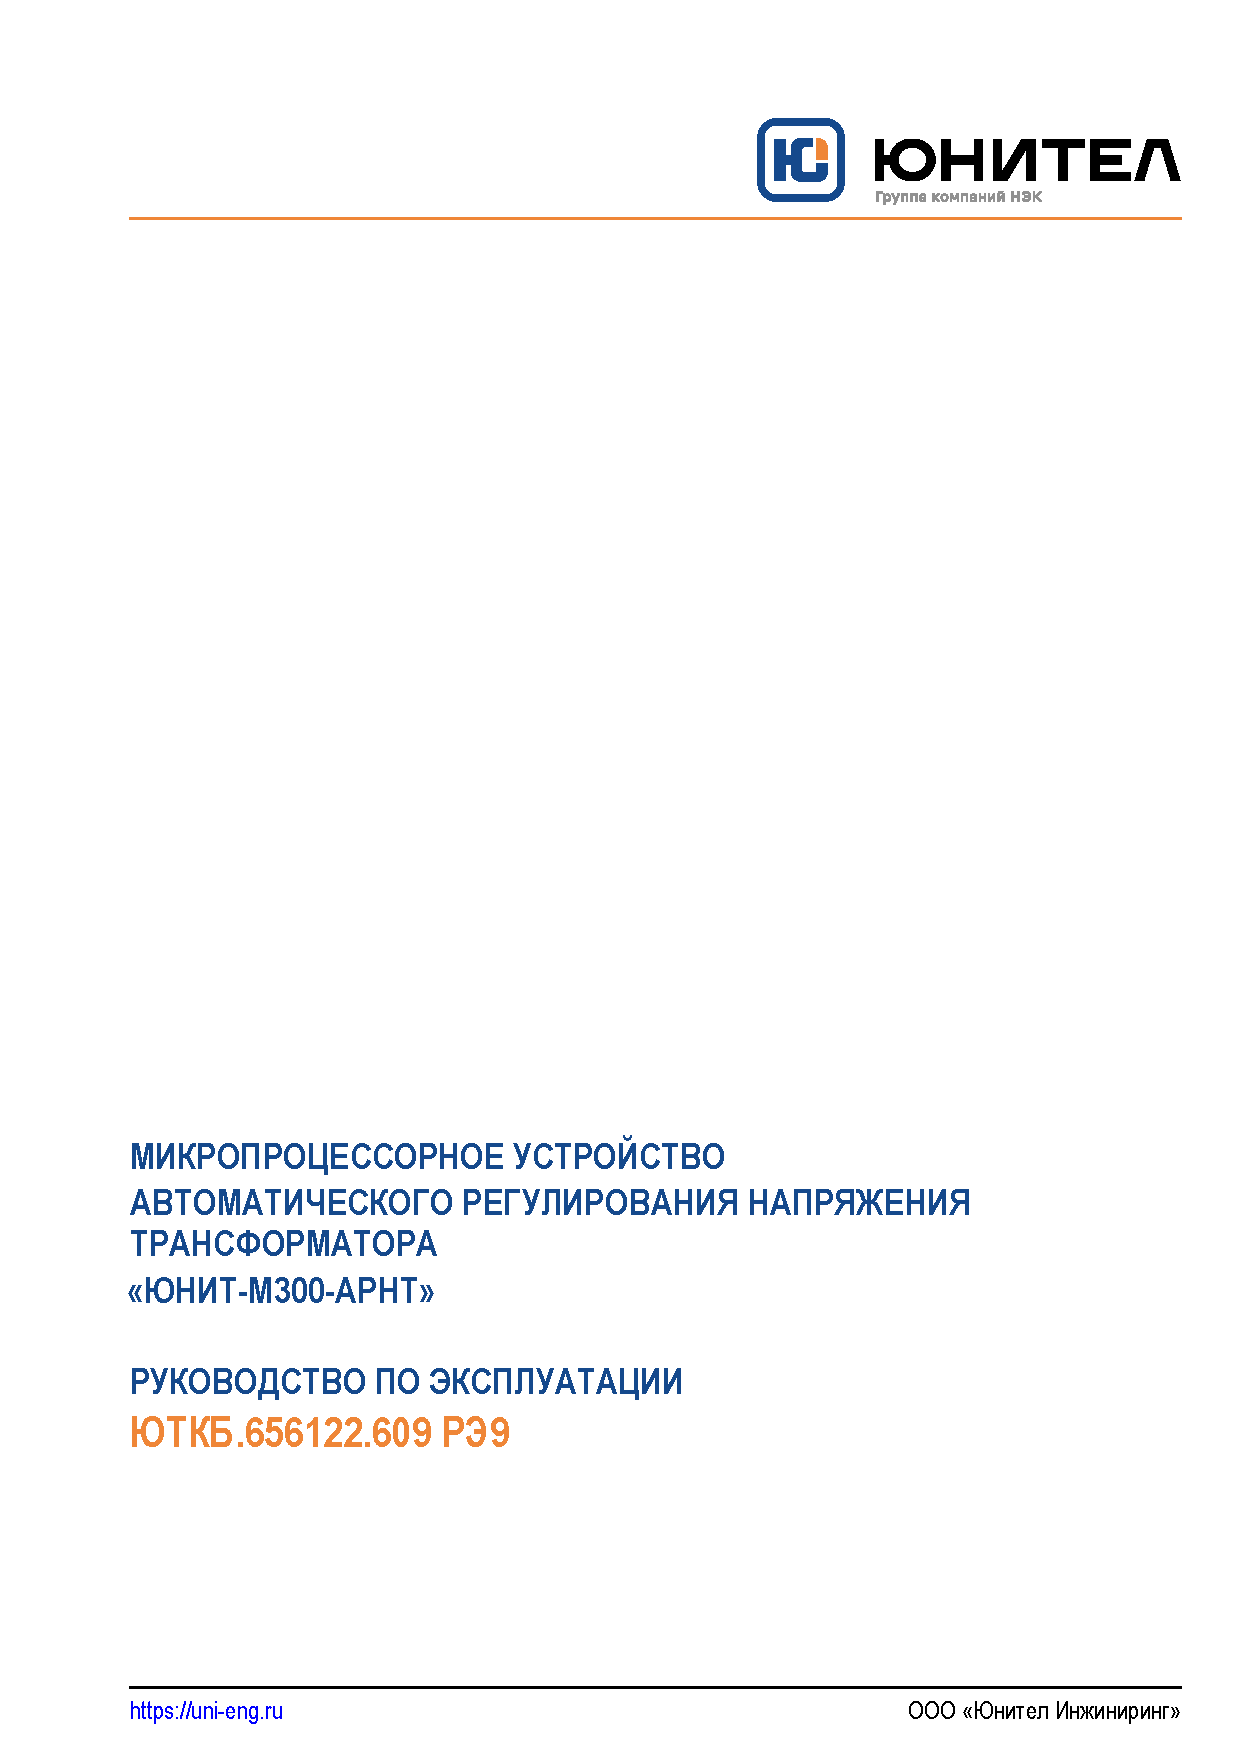
\includepdf[pages={1},width=0.5\textwidth, angle=90]{1.pdf} вставляем и поворачиваем pdf
%\begin{center}
%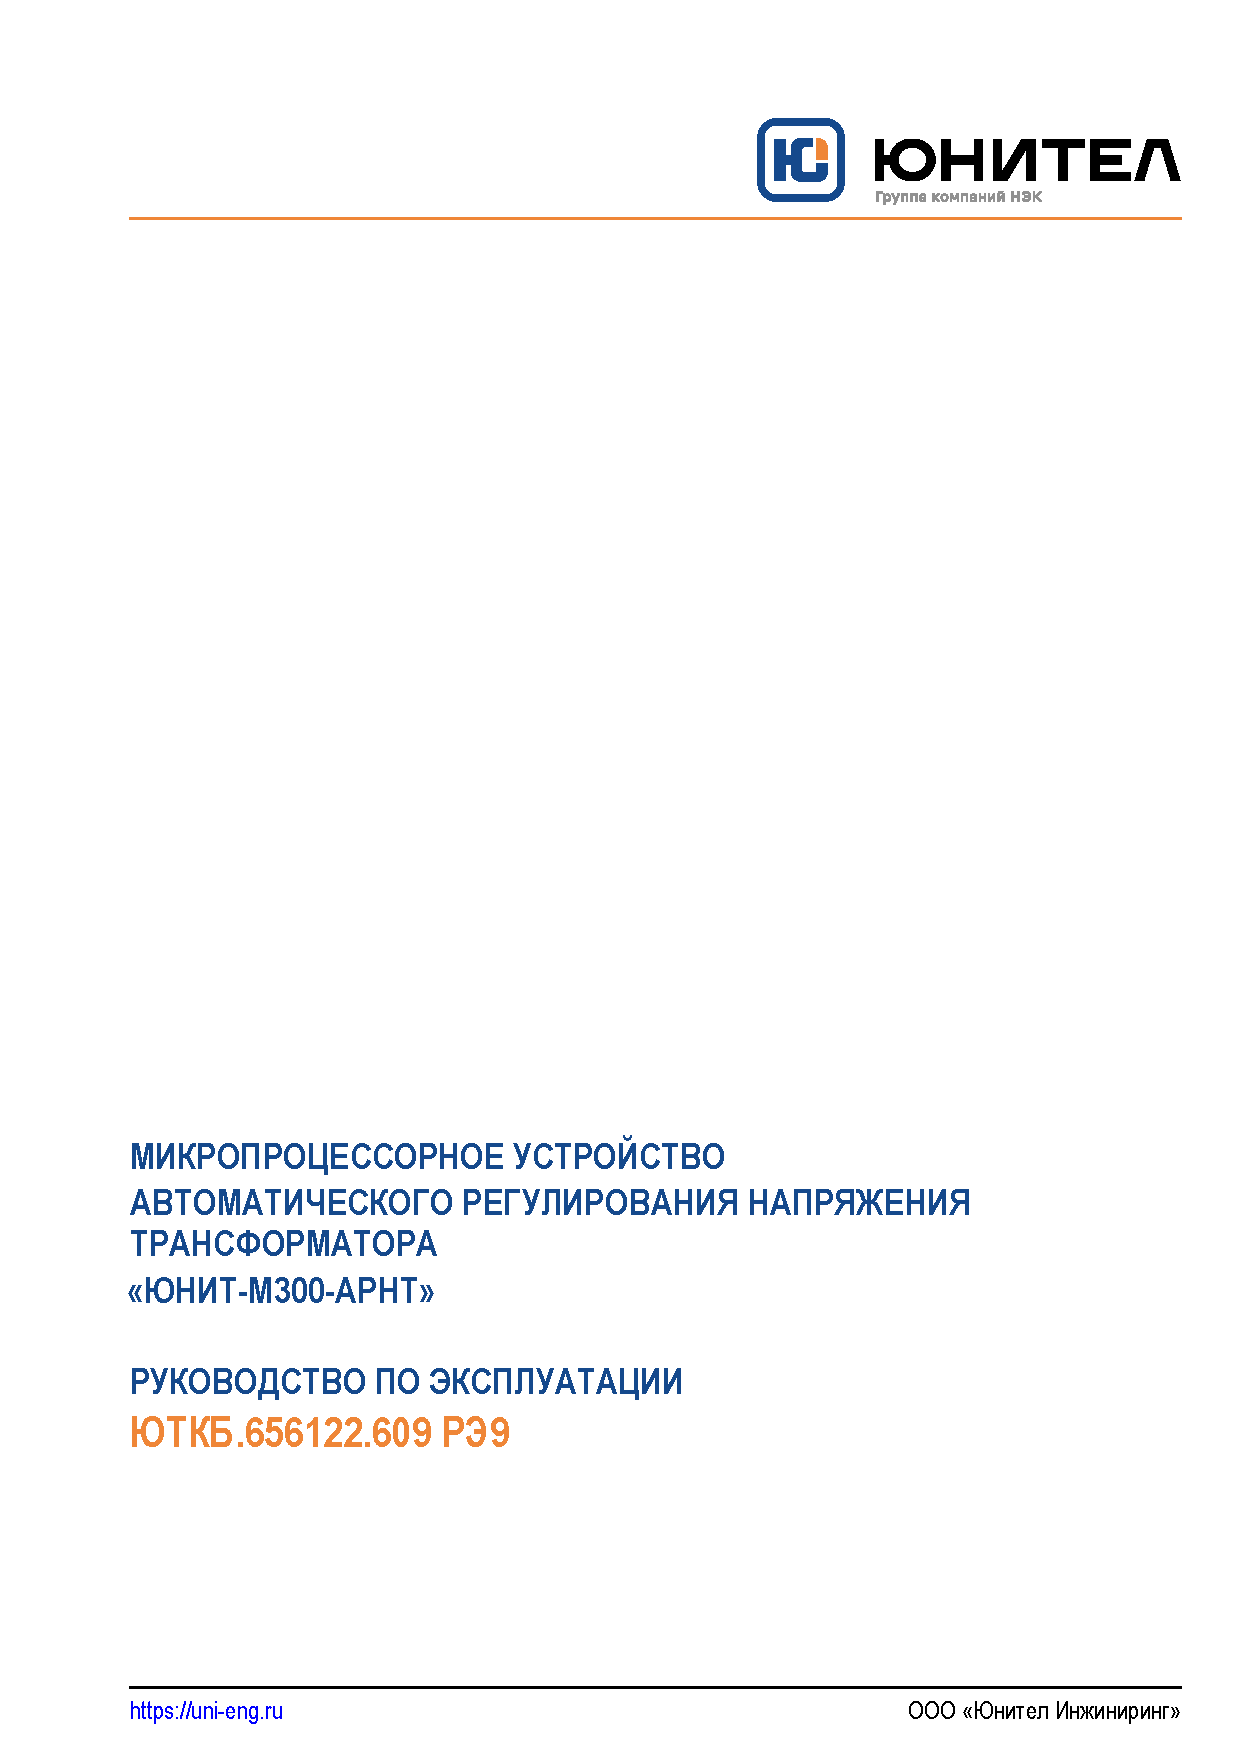
\includegraphics[width=1.4\textwidth]{1.pdf}
%\end{center}

\end{landscape}
\restoregeometry
